% =====================================================================
%  Paper A — Predictors != Interventions
%  Build: cd paper && latexmk -pdf main.tex   (or pdflatex + bibtex)
% =====================================================================
\documentclass{article}
\usepackage{iclr2027_conference,times}
% R38 (user): the sty forces \flushbottom (its l.54); on pages whose natural
% content runs short (e.g. p5 — Figure 1 float + start of §4.2) the elastic
% glue around floats/section heads stretches into a big mid-page hole.
% \raggedbottom must come AFTER the sty for the same reason.
\raggedbottom
\usepackage[utf8]{inputenc}
\usepackage[T1]{fontenc}
\usepackage{natbib}   %% \citet / \citep (author-year)
\usepackage[hypertexnames=false]{hyperref}
\hypersetup{hidelinks}
\usepackage{url}
\usepackage{booktabs}
\usepackage{amsfonts,amsmath,amssymb}
\usepackage{amsthm}
\newtheorem{claim}{Claim}
\theoremstyle{plain}
\newtheorem{lemma}{Lemma}
\newtheorem{corollary}[lemma]{Corollary}
\theoremstyle{definition}
\newtheorem{assumption}{Assumption}
\theoremstyle{remark}
\newtheorem{remark}{Remark}
\newtheorem{observation}{Observation}
\usepackage{nicefrac}
\usepackage{microtype}
\usepackage{enumitem}
\usepackage{graphicx}
\usepackage{algorithm}
\usepackage{algpseudocode}
\usepackage{placeins}
\graphicspath{{../figures/}{./}}

\hypersetup{
  pdftitle={Observation Does Not Imply Control: The Dynamics of
            Directional Curvature Interventions at the Edge of Stability},
  pdfauthor={}
}

\newcommand{\lmax}{\lambda_{\max}}
\newcommand{\lraw}{\ensuremath{\lambda_{\mathrm{raw}}}}
\newcommand{\lref}{\ensuremath{\lambda_{\mathrm{ref}}}}
\newcommand{\lstep}{\ensuremath{\lambda_{\mathrm{step}}}}
\newcommand{\lhatg}{\hat{\lambda}_{\mathbf{g}}}
\newcommand{\lhatd}{\hat{\lambda}_{\Delta\theta}}

% R42 table-readability helpers.
% These have no effect unless explicitly invoked inside a local table group.
\newcommand{\RTableTopGap}{%
  \setlength{\abovetopsep}{2pt}%
}
\newcommand{\RTableDenseRules}{%
  \setlength{\aboverulesep}{.55ex}%
  \setlength{\belowrulesep}{.75ex}%
}

\hypersetup{pdfauthor={}}

\title{Observation Does Not Imply Control:\\ The Dynamics of Directional Curvature\\ Interventions at the Edge of Stability}

\author{Anonymous authors\\
Paper under double-blind review}

\begin{document}
\maketitle

\begin{abstract}
Curvature estimation has made sharp directions increasingly accessible
in neural-network optimization, but a measured direction need not
respond predictably to intervention. We study directional gradient
edits at the Edge of Stability (EoS). In a full-batch MLP,
fixed-divisor edits provide an interventional test of known
preconditioned-stability algebra: conditional on trajectories that
exhibit the corresponding sign-flip orbit, late raw sharpness tracks
its predicted location $2d/\eta$, while orbit survival is separate and
is not explained by the reduced model. In stochastic
ResNet-18/CIFAR-100 training, an engaged rank-1 attenuation arm and
wider raw-divisor top-eigenspace rescalings through $k{=}20$ show no
statistically resolved reduction in the tested sharpness diagnostics
at the canonical operating point; the wider rescaling rule is not
unconditional pure damping because below-target directions receive
bounded sign-reversed amplification. We use SAM as a
sharpness-reduction control: the tested $\pm H\mathbf{g}$ first-order
corrections do not reproduce its ResNet response, and the sampled
linSAM-to-SAM interpolation associates lower sharpness with increasing
weight on the finite re-query residual bundle. This pathwise
decomposition does not isolate a unique nonlinear mechanism and does
not transfer in the same form to the LayerNorm ViT control. These
results distinguish observing curvature from predicting the response
to a specific curvature intervention, within the tested systems,
measurements, and intervention rules.
\end{abstract}

\section{Introduction}
\label{sec:intro}
Modern curvature estimators make the sharp directions responsible for
instability in neural-network optimization increasingly accessible.
Measuring a sharp direction, however, does not by itself guarantee
effective control under the intervention families tested here. Gradient descent at the
Edge of Stability (EoS) provides a natural testbed for this question:
the Hessian top eigenvalue $\lmax$ climbs toward the linear-stability
threshold $2/\eta$ and oscillates there while loss decreases
non-monotonically \citep{cohen2021eos,damian2023selfstab}. This
accessibility motivates a natural intervention: modify the gradient
along sharp Hessian directions in an attempt to control
sharpness; whether this intuition holds for neural-network
optimization is the subject of this paper.

We organize the experiments around a known piece of threshold algebra,
stated here for reference
\citep{cohen2022adaptive,nonEuclidean2026eos}: a divisor-$d$ edit along
a sharp direction rescales the effective local step to
$\eta_{\mathrm{eff}}=\eta/d$, so the linear-stability location of a
sign-flip period-2 orbit moves from $2/\eta$ to
\begin{equation}
\lambda_{\mathrm{crit}}=2d/\eta=2/\eta_{\mathrm{eff}},
\label{eq:etacrit}
\end{equation}
Lemma~\ref{prop:boundary} establishes this
orbit location in the 2-D self-stabilization reduction; our
contribution is a feedback-free interventional test of the
reduced-map orbit-location prediction on trajectories that exhibit
the corresponding sign-flip behavior
(\S\ref{sec:control}), and of what replaces this picture in the
stochastic regime (\S\ref{sec:stochastic}).\looseness=-1

Across our experiments, two failure modes emerge within the tested
intervention families:
\begin{itemize}[leftmargin=*,itemsep=1pt]
\item \emph{Geometry relocation.} The edit acts but moves its own
target: damping a sharp direction by $1/d$ relocates the sign-flip
stability boundary from $2/\eta$ to $2d/\eta$, and surviving
trajectories track the moved boundary upward instead of
descending: the intervention moves the very stability constraint it
was designed to control.
\item \emph{Stochastic mismatch between the measured curvature
direction and the effective control response.} At
the reference stochastic operating point, the edited eigenspace
carries little of the current minibatch gradient and the intervention
produces no resolved sharpness reduction; the small gradient share
diagnoses weak immediate actuation but does not by itself explain the
long-horizon null (\S\ref{sub:inertness}).
\end{itemize}
The two modes are therefore limiting
cases connected by an exploratory regime sweep, rather than disjoint
categories assigned by regime label. Their boundaries are system- and
protocol-dependent: a ViT control reproduces the unresolved damping
response and even shows the relocation direction at its
high-curvature point, yet the ResNet linSAM--SAM separation does not
transfer in the same form. The organization summarizes the tested
outcomes; it is not a predictive classifier for unseen systems or
protocols, nor an assertion that sharpness is uncontrollable: full-batch
rank-1 amplification and stochastic SAM both show that sharpness can
be reduced by intervention in the tested settings.\looseness=-1

The central message of this work is that curvature is not an external
quantity available for direct manipulation: the optimizer dynamics
that create a sharp direction are themselves altered when that
direction is modified. In stochastic ResNet-18/CIFAR-100
training, the corrected rank-1 attenuation arm and the tested wider
raw-divisor rescalings through $k{=}20$ show no statistically
resolved sharpness reduction, and neither $\pm\,H\mathbf{g}$
first-order correction reproduces SAM's; along a direct
linearized-to-full-SAM interpolation the four sampled arm means
decrease (with no large change in the directly instrumented
pre-update norm), providing a pathwise residual-bundle decomposition
that a LayerNorm ViT control shows to be system-dependent rather than
universal.\looseness=-1

\paragraph{Contributions.}
\begin{itemize}[leftmargin=*,itemsep=1pt]
\item \textbf{Intervention map across regimes.} We organize the
tested directional interventions by two observed response patterns:
relocation of the sign-flip orbit location in the full-batch
reduction, and an unresolved sharpness response under the tested
stochastic eigenspace rescalings: a descriptive organization, not a
predictive regime classifier (the exploratory batch-size sweep shows
that weak instantaneous actuation alone does not determine the
long-horizon response). At the canonical ResNet-18/CIFAR-100
operating point, neither the engaged rank-1 attenuation arm nor the
wider $k{\le}20$ raw-divisor signed eigenspace rescalings (which are
not unconditional pure damping) show a statistically resolved
sharpness reduction; the edited subspace's small gradient share is an
actuation diagnostic, not an explanation of the long-horizon
null.\looseness=-1
\item \textbf{Conditional interventional test of orbit relocation.}
The shift $2/\eta \to 2d/\eta$ is known stability algebra rather than
a new threshold law. We test its network-level orbit-location
consequence without adaptive feedback: among fixed-divisor
trajectories that exhibit the corresponding stationary sign-flip
behavior, late raw sharpness tracks the predicted location, while
orbit survival is reported separately and is not explained by the
reduced model.\looseness=-1
\item \textbf{Pathwise SAM decomposition.} Neither tested
$\pm H\mathbf{g}$ first-order correction reproduces SAM's ResNet
sharpness reduction. Across the sampled linSAM-to-SAM interpolation,
increasing the finite re-query residual bundle is accompanied by
decreasing sharpness. This identifies what differs along this
particular path, not an isolated universal SAM mechanism; the ViT
control gives a different decomposition.\looseness=-1
\end{itemize}\looseness=-1\looseness=-1

\section{Related work and positioning}
\label{sec:related}
\paragraph{EoS core and its stochastic counterpart.} Prior EoS
analyses characterize how sharpness emerges and stabilizes under a
given optimizer: the Hessian spectrum governs the stability limit
($\lmax\!\to\!2/\eta$) \citep{lewkowycz2020catapult,cohen2021eos};
progressive sharpening, self-stabilization, and saturation theorems
\citep{li2022sharpness,damian2023selfstab,agarwala2022second};
simplified-model and bifurcation-theoretic accounts
\citep{chen2023beyond,ahn2023threshold,song2023trajectory};
sign-flip/route-to-chaos descriptions
\citep{kalra2023phase,kalra2025universal}; implicit
sharpness-minimization \citep{arora2022understanding} and
time-averaged central flows \citep{cohen2025central}: largely
deterministic/full-batch analyses, with stochastic counterparts in
batch sharpness \citep{andreyev2024eoss,andreyev2026momentum} and
preconditioned top eigenvalues \citep{cohen2022adaptive}. We study an
interventional rather than algebraic extension of this literature:
after modifying the optimizer along a measured sharp direction, does
the original sharpness mechanism remain intact? Static
preconditioning already implies that rescaling an update direction
changes the relevant spectral stability quantity
\citep{cohen2022adaptive}, and recent work develops preconditioned
GD as a generalized EoS setting \citep{nonEuclidean2026eos}; we do
not claim the $2d/\eta$ threshold shift itself as novel. Our
full-batch contribution is the feedback-free fixed-divisor test of
whether network trajectories exhibiting the relevant sign-flip
behavior realize that location, together with an explicit separation
between orbit location and orbit survival. Existing stochastic-EoS
analyses characterize how minibatch noise and momentum modify the
stability statistics of a fixed optimizer
\citep{andreyev2024eoss,andreyev2026momentum}. Our batch-size map
does not derive a competing stochastic equilibrium law; it is an
exploratory intervention study over selected operating points and
should not be read as a stochastic extension of the 2-D full-batch
theorem.

\paragraph{Directional curvature edits.} CDAT \citep{roulet2024cdat}
uses curvature along the update as a step-size denominator and embraces
the $2/\eta$ threshold; critical sharpness \citep{kalra2026scalable}
defines $\lambda_c$ via line search and states the Rayleigh identity we
repurpose into a single-HVP monitor. \citet{song2025bulk} remove dominant
Hessian-eigenvector components from the SGD update and observe
constrained optimization with unconstrained sharpness: the
$d\!\to\!\infty$ limit of our damping family. Our subspace-energy
diagnostic differs
operationally: it measures the current minibatch gradient's energy on
the instantaneous top-$k$ eigenspace of the current Hessian estimate,
whereas \citet{song2025bulk} target a persistent dominant subspace
aggregated over training; a small instantaneous share is not
inconsistent with their bulk-subspace observations. Our finite
raw-divisor rescalings are not equivalent to removing a persistent
dominant subspace, and the stochastic wider-rank rule can change
sign below target. We therefore use \citet{song2025bulk} primarily
to position the broader question of Hessian-subspace interventions
rather than to claim a direct algorithmic continuation between the
two procedures. We vary the
strength, sign, rank, sensing source, and stochasticity of the edit.\looseness=-1

\paragraph{Measurement, normalization, and SAM.} Warm-started power
iteration tracks accurate estimates of $\lmax$ at a few HVPs per step at 3B scale
\citep{ramasinghe2026taming}. Large batches find sharper minima
\citep{keskar2017largebatch} with known caveats \citep{dinh2017sharp};
normalization reshapes sharpness \citep{wei2019bn,lyu2022spherical}.
SAM \citep{foret2021sam} is our escape benchmark; \citet{long2024sam}
derive a SAM-specific EoS cutoff that SAM empirically tracks. We test
vanilla SAM; scale-invariant and output-level variants
\citep{kwon2021asam,du2022saf} share a related amplifying structure, so our
negative attenuation result does not transfer to them.\looseness=-1

Closest to our stochastic analysis, \citet{agarwala2023sam} derive the
sharpness level at which SAM stabilizes idealized dynamics as a function of
$\eta$ and $\rho$, \citet{wen2023sharpness} isolate which parameter blocks
SAM must perturb to retain sharpness reduction in deterministic settings, and
\citet{bartlett2023dynamics} analyze SAM's bounce-and-drift dynamics in
minimal non-convex problems. Our ladder differs in aim: rather than
characterizing SAM itself, we interpolate between a linearized and the
full SAM update to test which update difference carries the endpoint
separation along a controlled interpolation.\looseness=-1

\section{Setup}
\label{sec:setup}
\paragraph{Testbeds.}
Three testbeds carry the paper: (i)~a tanh MLP
$[20\!-\!256\!-\!256\!-\!1]$ teacher--student regression under
full-batch GD; (ii)~a CIFAR-adapted ResNet-18 ($3{\times}3$ stride-$1$
stem, no max-pooling; $11.2$M parameters) on CIFAR-100, trained under
the deterministic $5000$-step replayed mini-batch protocol
(hyperparameters: Appendix~\ref{app:hyper}), a short constant-lr
mechanistic protocol chosen to expose
stationary sharpness dynamics and studied throughout
\S\ref{sec:stochastic}; the 200-epoch external check
(\S\ref{sub:external}) tests the SGD/damping/SAM ordering under a
standard recipe; and
(iii)~\texttt{timm} ViT-tiny (LayerNorm) on CIFAR-100 as a
cross-system control (\S\ref{sub:external}). Additional
architectures used only for instrumentation and ablations
(PreAct-ResNet, ConvNeXt, matched-step X-SAM projector ablation) are described in the
appendices.

\paragraph{Sharpness quantities.}
Three sharpness quantities appear, and they are different objects:
$\lraw=\lmax(H)$ is the raw Hessian top eigenvalue
governed by the full-batch $2/\eta$ law; $\lref=
\lmax(H_R)$, the ARPACK top eigenvalue on a fixed $512$-example
evaluation batch (model in eval mode), is the cross-method
diagnostic used in the stochastic experiments, reported against the
heavy-ball reference line $2(1{+}\mu)/\eta$, used as a fixed
reference, \emph{not} a
theoretical constraint on $H_R$; and
$\lstep=\mathbb{E}_{B}[\mathbf{g}_{B}^{\!\top}H_{B}
\mathbf{g}_{B}/\|\mathbf{g}_{B}\|^{2}]$ is the batch sharpness, constrained
by EoSS theory for SGD(-momentum) dynamics, which stabilizes at $2/\eta$
momentum-free and
plateaus between $2(1{-}\mu)/\eta$ and $2(1{+}\mu)/\eta$ with
momentum \citep{andreyev2024eoss,andreyev2026momentum}; we evaluate it
as a diagnostic along all optimizer trajectories, including SAM's,
without implying that SAM's update obeys the same $2/\eta$
boundary. Because $H_R$ is evaluated through the model's stored
BatchNorm state, $\lref$ is a state-dependent protocol diagnostic
rather than a parameter-only invariant of the network function.
Appendix~\ref{sub:bnproto} shows that changing only the
BatchNorm-statistics convention can materially change its numerical
level; cross-method comparisons are therefore interpreted only under
the stated matched protocol. A three-fixed-batch calibration in
Appendix~\ref{sub:crossbatch} shows comparable but non-identical
scalar levels across batches, so $\lref$ is used as a reproducible
protocol-specific cross-method diagnostic, not as a population Hessian
eigenvalue. One further
distinction matters: the fixed-batch gradient used by the curvature
monitor and the current stochastic training gradient used to measure
intervention energy are different objects: the former aligns with the
top eigenvector in the EoS regime, the latter nearly never does under
bs-128 noise (\S\ref{sub:inertness}). Table~\ref{tab:quantities}
summarizes the three.\looseness=-1

\begin{table}[t]
\centering
\small
\begin{tabular}{@{}lll@{}}
\toprule
Symbol & Meaning & Used for \\
\midrule
$\lraw$ & full Hessian top eigenvalue & full-batch GD boundary \\
$\lref$ & fixed-batch ARPACK $\lmax$ & cross-method diagnostic \\
$\lstep$ & batch gradient curvature & EoSS quantity (SGD--momentum); diagnostic for all arms \\
\bottomrule
\end{tabular}
\caption{The three sharpness quantities.}
\label{tab:quantities}
\end{table}

\paragraph{Operational meaning of control.}
Throughout the paper, ``control'' means an intervention intended to
reduce the reported raw or reference sharpness quantity; it does not
denote control-theoretic controllability or closed-loop stability,
nor do we identify raw Hessian sharpness with a
parameterization-invariant generalization measure. In particular, a
directional rescaling can regulate an effective or preconditioned
stability quantity while raw $\lmax$ increases. We therefore describe
such an outcome as a failure only with respect to the stated
raw-sharpness reduction objective.\looseness=-1

\paragraph{Curvature and statistics.} $\lmax$ via power iteration +
Pearlmutter HVP on the MLP path (cross-validated against ARPACK to
$\le3\times10^{-7}$ relative); deterministic ARPACK at ResNet-18
scale. Headline reference-sharpness comparisons use $n{=}5$ seeds
(mean$\pm 95\%$ CI); instrumented batch-sharpness reruns use $n{=}3$
unless flagged in the run manifest. For ordinary paired arm
comparisons, we first form one per-seed difference using matched seed
IDs and the experiment's prespecified summary window, then report the
mean paired difference with a two-sided 95\% $t$ confidence interval;
we call a paired difference statistically resolved only when this 95\%
CI excludes zero. Practical-equivalence claims are evaluated
separately with TOST at $\alpha{=}.05$ on the same paired per-seed
differences. For TOST, the corresponding 90\% CI is compared with the
prespecified design margin, set before the
rank-$k$ equivalence experiments to one quarter of SAM's
late-window reduction in the protocol at hand (numeric margins,
their relation to the SGD reference levels, and the sensitivity
analysis at stricter and looser margins, under which no tested arm
satisfies equivalence at the stricter one-eighth margin, are in
Appendix~\ref{sub:tostmargin}). Thus 95\% CIs support ordinary difference
claims, whereas 90\% CIs are used only for equivalence testing. The
$m{=}4$ batch-sharpness estimate is
intentionally compute-limited and consequently noisy (Monte-Carlo
variance and a subsampling calibration: Appendix~\ref{par:mcal}).
Training-time accuracy curves use a fixed $2{,}000$-example test subset only for
post-hoc visualization; all headline accuracy results use the full test
set. A 95\% CI containing zero is reported only as ``not statistically
resolved''; particularly for $n{=}3$ supporting arms, this is not
evidence that the effect is absent or negligibly small. The appendix
contains many secondary ablation comparisons. Unless a comparison is
explicitly identified as prespecified, its confidence interval should
be read as per-comparison descriptive evidence; we do not claim
family-wise error control across the full ablation suite.\looseness=-1

\paragraph{Protocol semantics.}
In the stochastic experiments, the corrected rank-1 arm is an engaged
attenuation test, whereas the $k{>}1$ experiment uses the no-floor
raw-divisor signed rescaling defined in \S\ref{sub:inertness}.
Current-minibatch-sourced eigenvectors are refreshed every $N{=}20$
steps; legacy sensing, clamp variants, and complete measurement
semantics are detailed in Appendices~\ref{app:robust}
and~\ref{app:stoch}.\looseness=-1

\section{Full-batch GD: fixed-divisor edits test a reduced-map orbit-location prediction}
\label{sec:control}

\subsection{Reduced-model prediction}
\label{sec:theory}
\begin{lemma}[Reduced-map orbit location under directional rescaling; conditional on the 2-D self-stabilization recurrence of \citet{damian2023selfstab}]
\label{prop:boundary}
Assuming an isolated positive top eigenpair, window-fixed edit
strength, accurate top-eigenvector sensing, and the reduced
recurrence specified in Appendix~\ref{app:theory}, every sign-flip
period-2 orbit of that recurrence satisfies $\lambda^{*}=2d/\eta$
with $d=1/(1-\gamma)>1$ for damping ($\gamma\in(0,1)$), and
$\lambda^{*}=2/((1+\alpha)\eta)<2/\eta$ for the sign-reversed
amplifying edit ($\gamma=-\alpha<0$).
\end{lemma}

\noindent\fbox{\parbox{0.97\linewidth}{\small
Lemma~\ref{prop:boundary} is an orbit-location statement, not a
trajectory-level theorem: the reduced orbit is not proven attractive,
and the network evidence in \S\ref{sub:fixedd} is interventional.}}\looseness=-1

As organized in \S\ref{sec:intro}, damping rescales the effective
step along the sharp direction to $\eta/d$, moving the sign-flip
condition to $2d/\eta$; the edit's
contribution to the slow $y$-drift has zero cycle mean at odd order
and only renormalizes the amplitude coefficient at even order
(Appendix~\ref{app:theory}), so the sign-flip orbit location remains
$\lambda^{*}=2d/\eta$.\looseness=-1

The reduced orbit is indeed not guaranteed to attract: the
corresponding orbit is repelling under the full two-dimensional
Jacobian, so attraction in the network must involve higher-order
effects omitted by the reduction (gap~G4), and the lemma makes no
claim that the orbit attracts nearby trajectories, that a network
trajectory reaches it, or that the reduced recurrence explains the
observed basin of survival. Section~\ref{sub:fixedd} tests only the
orbit-location prediction, while separately reporting which
fixed-divisor trajectories survive.\looseness=-1

\subsection{Fixed-divisor interventional test}
\label{sub:fixedd}
The adaptive rule $d=\hat{\lambda}/(2/\eta)$ enforces
$\hat{\lambda}/d=2/\eta$ whenever the gate is active, so its trajectory
cannot by itself test the predicted boundary shift. We therefore remove
this feedback and hold $d=d_{\mathrm{fix}}$ constant while keeping the
edit and sensing procedure unchanged. On-orbit cells track the
predicted location $\lambda^{*}=2d_{\mathrm{fix}}/\eta$
(Fig.~\ref{fig:etad}a), and a fixed divisor matched to the adaptive
arm's realized mean reaches the same sharpness scale, whereas
intermediate divisors diverge on all seeds even though the adaptive
controller remains stable. Thus orbit location and orbit
survival are distinct effects: the fixed divisor tests the former,
while the adaptive feedback affects the latter.

This separation persists as a conditional orbit-location observation
across the $\eta\times d$ grid: seven cells exhibiting the
corresponding stationary sign-flip behavior lie within
$0.95$--$0.99$ of the predicted location; two additional surviving
cells are off the relation, and the remaining cells diverge
(Fig.~\ref{fig:etad}). Full per-cell survival counts and
device-sensitive boundary cases are in
Appendix~\ref{app:ampdetails}. We therefore do not
interpret Fig.~\ref{fig:etad} as showing that fixed-divisor dynamics
generally converge to $2d/\eta$: it shows that, conditional on the
observed trajectory entering the corresponding sign-flip regime, its
late location agrees closely with the reduced-map prediction. Orbit
entry, attraction, and survival remain outside
Lemma~\ref{prop:boundary}; the ``on-orbit'' and trajectory labels in
Fig.~\ref{fig:etad} are descriptive summaries rather than outcomes of
an independently preregistered orbit-classification test, so the
fixed-divisor experiment is used as conditional evidence about orbit
location only.\looseness=-1

The survival window is itself structured (Fig.~\ref{fig:etad}b):
divergence concentrates at large $\eta d$, stability is non-monotone
in $d$, and marginal cells are device-numerics sensitive, so the
higher-order dynamics bounding the orbit's basin
(Remark~\ref{rem:scope}, Appendix~\ref{app:theory}) act well beyond
the lemma's orbit-location content. A delayed-onset control
addresses the possibility that the fixed-$d$ failures are caused
simply by intervening too early: switching the adaptive arm to fixed
$d\in\{2.5,3\}$ at its measured natural gate-opening step still
yields no survivors at either $d$, while the adaptive rule remains
stable from the same state: stabilization is attributable to
the $\hat\lambda$-dependent feedback itself, not to delayed
intervention or warm-up (Appendix~\ref{app:ampdetails}).\looseness=-1

\begin{figure}[!t]
\centering
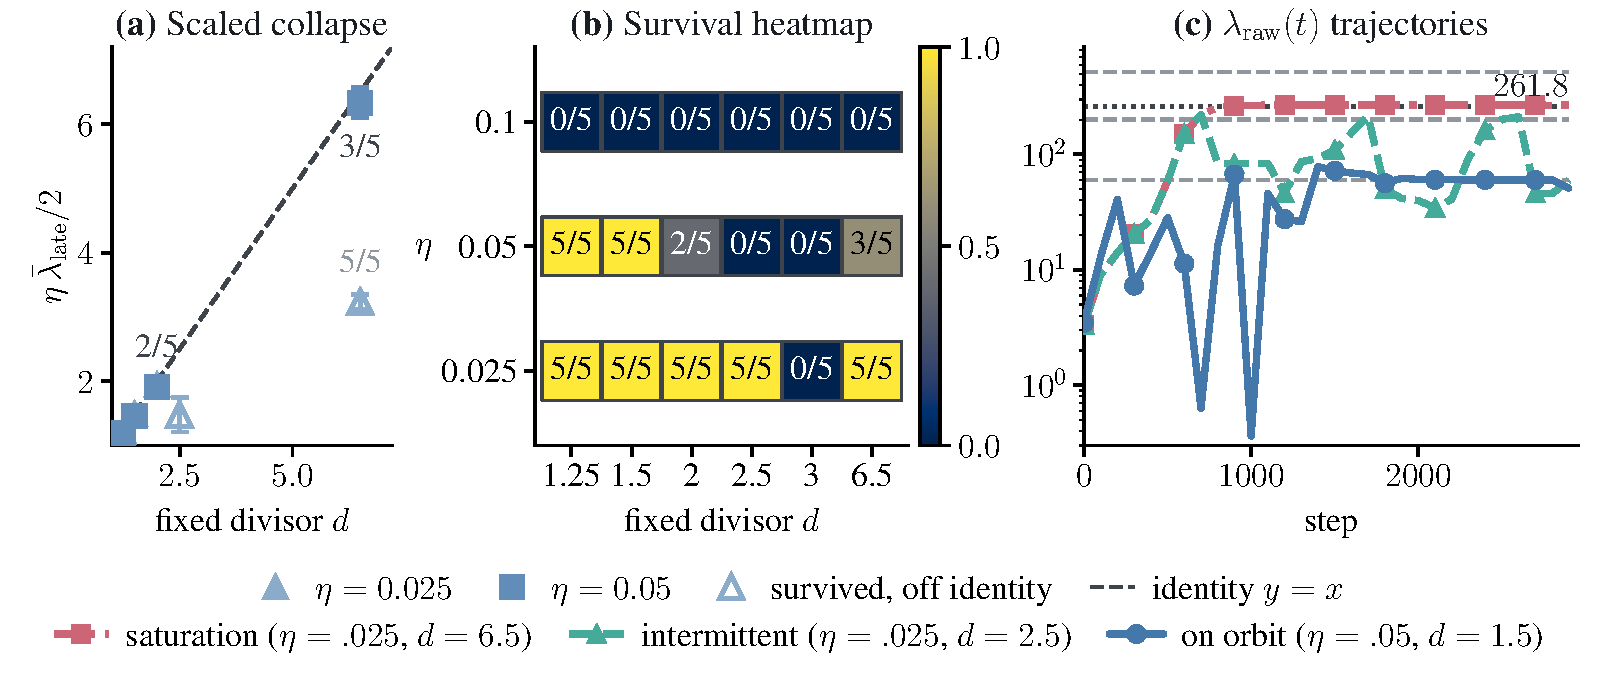
\includegraphics[width=0.95\linewidth]{47_etad_collapse.pdf}
\caption{Unified fixed-divisor grid (MLP full-batch; one CPU round,
float32; $n{=}5$ seeds per cell, $3000$ steps;
$\eta\in\{0.025,0.05,0.1\}$,
$d_{\mathrm{fix}}\in\{1.25,1.5,2,2.5,3,6.5\}$).
\textbf{(a)}~Dimensionless late-window level $\eta\bar\lraw/2$ vs.\
$d_{\mathrm{fix}}$: cells that settle onto a stationary orbit track
the identity (filled; ratios $0.95$--$0.99$); two cells at
$\eta{=}0.025$ survive off it (open; ratios $0.59$ and $0.50$, the
latter at $\lraw\approx260$).
\textbf{(b)}~Survival counts $n_{\mathrm{surv}}/5$: divergence
concentrates at large $\eta d$ (per-cell counts in
\S\ref{sub:fixedd}). \textbf{(c)}~Representative $\lraw(t)$ trajectories
(seed $0$, late means match the grid; predicted levels
$2d_{\mathrm{fix}}/\eta$ dashed, rank-1 escape ceiling dotted;
delayed-onset control: Appendix~\ref{app:ampdetails}). The three
trajectory types in panel~(c) are encoded redundantly by hue and line
style/marker.}
\label{fig:etad}
\end{figure}

\subsection{Sign reversal: accurate rank-1 attenuation raises the
observed late-window sharpness in the tested full-batch system;
amplification descends}
\label{sub:amp}\label{sub:rank1}
Reversing the sign gives the complementary reduced-model prediction:
amplification of the top-gradient component places the sign-flip orbit
below $2/\eta$. Experimentally, rank-1 amplification lowers the
late-window mean sharpness monotonically across $\alpha=0.25/0.5/1$
($n{=}5$; Fig.~\ref{fig:amp}, Table~\ref{tab:amp};
Appendix~\ref{app:robust}). The observed values do not quantitatively
follow the naive fixed-$\alpha$ orbit formula, a discrepancy that
grows with the edit strength, so we interpret this experiment as
consistent with the predicted sign and ordering over the tested
strengths, reading the reduced recurrence as a local qualitative
model rather than a globally accurate predictor of the edited
equilibrium magnitude.

Accurate rank-1 \emph{damping} (full batch) instead lets sharpness
grow
\emph{past} $2/\eta$ ($261.8\pm5.4$) while reaching a \emph{lower}
final loss than GD ($0.090$ vs.\ $0.111$): in this testbed, lower
loss does not require moving below the EoS threshold.\looseness=-1

\subsection{Robustness of the full-batch account}
\label{sub:sam}\label{sub:migration}
Several controls probe alternative explanations for the full-batch
response: proxy-driven norm caps do not move $\lraw$; inaccurate
update-direction sensing leaves the original EoS cap intact, whereas
accurate top-direction sensing produces the upward response;
orthogonal damping and short sensing lags preserve the qualitative
distinction; and a constructed separable multi-sharp control shows
that spectral migration is not required to obtain the observed
response in that controlled example; it is not a general
multi-eigenvalue extension of the reduced theory (Appendix~\ref{app:robust}).
Section~\ref{sec:stochastic} shows that the same sign-based response
does not extend to the canonical stochastic regime.

\section{Stochastic deep networks: limits of the sign-based account}
\label{sec:stochastic}

\subsection{No resolved sharpness reduction from the tested low-rank
rescalings}
\label{sub:scale}
We evaluate the canonical operating point using
two complementary diagnostics (trajectories:
Fig.~\ref{fig:r18}; per-arm seed counts are given in the figure
captions). Our primary reported
batch-curvature diagnostic is the \emph{batch sharpness} $\lstep$
(defined in \S\ref{sec:setup}), evaluated as our compute-limited
Monte-Carlo estimate ($m{=}4$ minibatches) along all arms, including
SAM. Its estimator freezes BatchNorm running statistics in eval mode
for reproducible HVP measurement (measurement protocol:
Appendix~\ref{sub:mconv}): we use the EoSS theory, which constrains
this quantity for SGD(-momentum) dynamics, to motivate the
measurement, not as an assertion that the measured scalar is exactly
the train-mode stability variable of every optimizer arm; for SGD it
is centered near the momentum-free boundary (late-window
distribution: Appendix~\ref{app:stoch}). The stochastic rescaling
controller retains the target $\lambda_{\mathrm{targ}}{=}2/\eta$ because
it defines the intervention inherited from the full-batch construction;
under $\mu{=}0.9$ this target is an intervention convention, not a
claimed unique or exact stochastic stability boundary: the momentum
plateaus $2(1{\mp}\mu)/\eta$ make the reference non-universal under
momentum (Appendix~\ref{app:stoch}). We
reserve \emph{attenuation} or \emph{damping} for an edit whose realized
directionwise scale is in $(0,1)$, use \emph{raw-divisor signed
rescaling} when the no-floor rule may reverse sign below target, and
use \emph{amplification} for the fixed-sign
$\mathbf{g}+\alpha(\mathbf{g}^{\top}v)v$ controls. Across the
central arms
the ordering is (Fig.~\ref{fig:bsarms}; instrumented reruns on
$n{=}3$ shared seeds): SAM resolves below SGD in
$\lstep$ (paired $\Delta_{\mathrm{SAM-SGD}}$ $-4.30$, 95\% CI
$[{-}6.70,{-}1.89]$); rank-1 damping with fixed-batch ARPACK sensing
shows no statistically resolved difference from SGD; every gradient-side
amplifying action along positive-curvature directions has an
above-SGD point estimate; the same
qualitative ordering holds for $\lref$ (full estimates in
Appendix~\ref{app:stoch}). The
damping null is not an engagement failure: ARPACK-based sensing
verifies persistent engagement of the edited directions on
every substantive step (an early power-iteration sensor defect and
its diagnosis are recorded in Appendix~\ref{app:stoch}).
A rank-1 attenuation control with periodically refreshed
current-minibatch-sourced sensing (the most recently sensed
direction is reused between $N{=}20$-step ARPACK refreshes on
training minibatches) likewise
leaves the outcome in the SGD band, so the null is not specific to a
single fixed reference eigenspace, though this refresh cadence does
not test per-step same-minibatch oracle sensing (engagement
diagnostics: Appendix~\ref{app:stoch}).\looseness=-1

\subsection{Top-eigenspace edits show weak per-step alignment at the canonical operating point}
\label{sub:inertness}
How strongly do the edits actuate the update? Under bs-128 noise the
instantaneous training gradient aligns with \emph{any} top-eigenvector
estimate at $|\cos|\!\approx\!0.008$ (median, late window), so the
edited subspace's share of the per-step gradient energy is minute:
even the top-$20$ eigenspace carries $<0.3\%$ under the live in-run
convention (per-$k$ shares: Table~\ref{tab:interp}). A separate
eval-mode checkpoint convention against a fixed eigenspace gives
substantially larger shares (top-$100$ ${\approx}24\%$); the two
quantities condition on different batches, model modes, and
eigenspaces and must not be compared as estimates of the same random
variable, and the effect of $k{>}20$ edits remains untested
(Appendix~\ref{sub:k100}).\looseness=-1

The energy share diagnoses the immediate update perturbation, not the
long-horizon null itself: across the batch-size
sweep the share stays near $10^{-4}$ over
$B\in\{128,\dots,2048\}$ (Table~\ref{tab:regimebridge}),
yet the same edit's paired outcome shifts from unresolved at
$B{=}128$ to a statistically resolved ${+}44.0$ at the
quasi-deterministic end: weak per-step actuation can coexist with
both null and non-null outcomes (full sweep: Appendix~\ref{app:stoch}).\looseness=-1

\begin{figure}[!t]
\centering
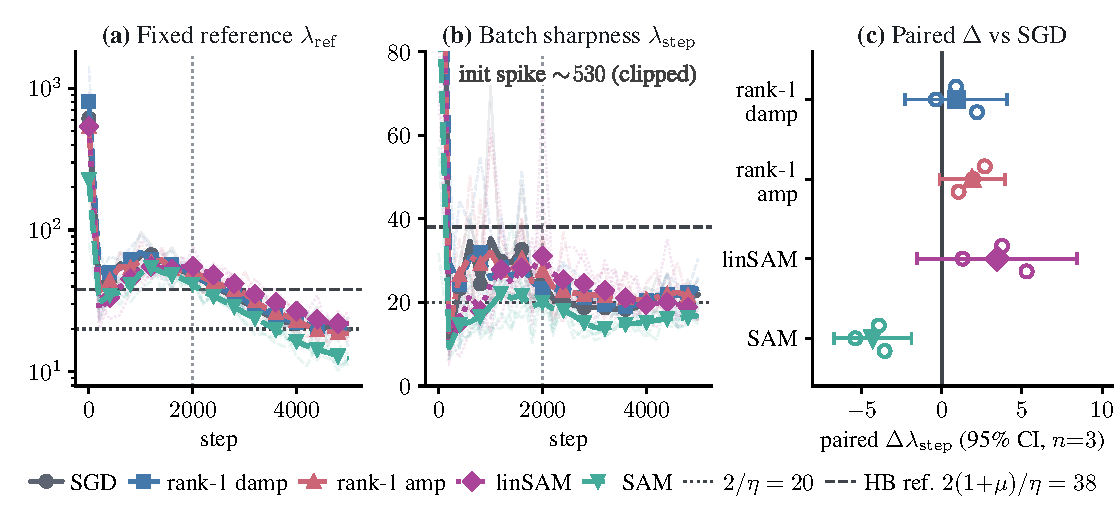
\includegraphics[width=0.95\linewidth]{43_bsharp_arms.pdf}
\caption{Batch sharpness across optimizer arms (deterministically
replayed mini-batch protocol, $5000$ steps; per-seed trajectories thin,
seed mean bold; late window $\geq2000$; $n$ per arm:
SGD/rank-1 damping/amplification $n{=}3$, SAM/linSAM $n{=}5$).
\textbf{(a)}~Fixed-reference \lref; \textbf{(b)}~the EoSS batch
sharpness $\lstep=\mathbb{E}_{B}[\mathbf{g}_{B}^{\!\top}H_{B}
\mathbf{g}_{B}/\|\mathbf{g}_{B}\|^{2}]$; \textbf{(c)}~late-window
paired differences $\Delta=\mathrm{arm}-\mathrm{SGD}$ on shared seeds
(open markers: per seed; marker+bar: mean and 95\% CI). SAM sits below
the SGD level (paired $\Delta_{\mathrm{SAM-SGD}}$ $-4.30$,
95\% CI $[{-}6.70,{-}1.89]$), rank-1 damping shows no statistically
resolved difference from SGD, and every
gradient-side amplifying action along positive-curvature directions
has a positive point estimate. The $2/\eta$ and
$2(1{+}\mu)/\eta$ lines are reference lines only; optimizer identity is
encoded redundantly by hue, line style, and marker.}
\label{fig:bsarms}
\end{figure}

A complementary coordinate is the realized gradient-side edit
magnitude $\|\mathbf{g}'-\mathbf{g}\|/\|\mathbf{g}\|$ (computed
exactly from the plant logs): the widest rescaling tested, rank 20,
actuates about $6\%$ per fired step, substantially smaller than the
measured linSAM and SAM corrections, yet magnitude alone does not
predict the outcome, since SAM produces a statistically resolved
downward shift in $\lstep$ whereas linSAM has an upward point
estimate; per-step actuation therefore remains a diagnostic rather
than a sufficient explanation of the response (every $k$, the
angles, and the momentum-buffer caveat:
Appendix~\ref{app:stoch}, Table~\ref{tab:actuationfull}).\looseness=-1

The wider-rank experiment extends the number of rescaled Hessian
directions under the same raw-divisor rule; it is not a pure-rank
ablation of unconditional attenuation, and its outcome reflects the
full rank-dependent rescaling rule (engagement changes with $k$;
per-direction firing fractions: Table~\ref{tab:interp}) rather than
an isolated causal effect of rank. For direction $i$ the
implementation uses $d_{i}=\hat\lambda_{i}/\lambda_{\mathrm{targ}}$
without a $\max(d_{i},1)$ floor and
$f_{i}=\mathrm{clip}(1-1/d_{i},-1,1)$, so directions with $d_{i}>1$
are attenuated whereas directions with $d_{i}<1$ receive bounded
sign-reversed amplification; we therefore refer to the $k{>}1$ arms as
raw-divisor signed eigenspace rescalings rather than pure rank-$k$
damping. The corrected rank-1 arm is different in practice: its sensed
divisor remains above one over the substantive engaged window
(Appendix~\ref{sub:engagement}), so that arm is an attenuation test.
Across $k{\le}20$, none of the raw-divisor rescaling arms has a
statistically resolved downward $\lref$ contrast; among them, only
$k{=}10$ satisfies the prespecified equivalence
criterion at this sample size and margin (TOST, $\alpha{=}.05$;
Fig.~\ref{fig:interp}, Table~\ref{tab:interp}). Rank-$k$
\emph{amplification} never reproduces SAM's shift toward lower
sharpness: the trend is toward higher sharpness, with the $k{=}20$
increase statistically resolved under the 95\% paired-CI criterion.
Directly measured outcome spectra show little
systematic spectral migration around the edit
(Appendix~\ref{app:stoch}), and the regime sweep of
Table~\ref{tab:regimebridge} is treated only as an exploratory
operating-point map, not a controlled causal trajectory from
stochastic to deterministic dynamics: the alignment measurements are
diagnostic rather than causal, and weak alignment is not claimed as
the mechanism of the long-horizon null.\looseness=-1

\FloatBarrier\looseness=-1

\subsection{Interpolating between linSAM and SAM: the finite re-query
residual bundle carries the ResNet transition}
\label{sub:sammech}
\label{par:rhosweep}
SAM serves here only as a contrasting sharpness-reduction control: it
reduces sharpness where the attenuating edits above do
not, and its update
expands to first order as $\mathbf{g}+(\rho/\|\mathbf{g}\|)H\mathbf{g}$,
which amplifies positive-curvature components (and attenuates
negative-curvature ones). Because $H\mathbf{g}$ reweights the full
spectrum with sign determined jointly by Hessian eigenvalues and
gradient components (including negative-curvature directions), this
correction is not the high-rank limit of the attenuation
experiments: it shows only that this specific $+\,H\mathbf{g}$ edit
is insufficient to reproduce SAM's reduction under this
protocol, not that high-rank attenuation as such fails. The
linearized arm ($\rho{=}0.05$ matched, one HVP per step, no
perturbed-point re-query) lands above SGD by a statistically
resolved paired contrast and ${\sim}12$ above
SAM (Fig.~\ref{fig:linsam}).
The SAM--linSAM
ordering persists across the tested radii $\rho\in[0.005,0.1]$, and
the re-query's nonlinear Taylor
residual remains comparable in magnitude to the
first-order correction throughout (Fig.~\ref{fig:rhosweep}); linSAM
is therefore an operational first-order comparator, not
evidence that SAM is well approximated by its first-order Taylor
expansion over the tested radii. BN-protocol controls with
bit-identical buffer trajectories show that matching the BN-state
evolution alone is insufficient to reproduce SAM's
level (Appendix~\ref{app:stoch}); these experiments form a sequence
of increasingly different intervention families, not a
magnitude-matched nested sufficiency test, and the first two do not
reproduce SAM's shift at this operating point.\looseness=-1

The opposite-sign correction
$\mathbf{g}-(\rho/\|\mathbf{g}\|)H_{B}\mathbf{g}$, with the same
nominal $\rho/\|\mathbf{g}\|$ scaling, likewise shows no resolved
reduction relative to SGD and leaves batch sharpness at the SGD level
(realized-magnitude caveat and full statistics:
Appendix~\ref{sub:rhosweepapp}); thus none of the tested low-rank
rescalings or full-rank $\pm H\mathbf{g}$ corrections reproduces
SAM's downward shift in this protocol.\looseness=-1

We next interpolate directly between the BN-matched linSAM and SAM,
$g_\tau=g_{\rm lin}+\tau\,(g_{\rm SAM}-g_{\rm lin})$, while holding
the BatchNorm protocol and RNG stream fixed. Across the four sampled
$\tau$ values, both reported sharpness means decrease; this associates
the endpoint separation with increasing weight on the finite re-query
residual bundle along this path, without isolating its nonlinear
constituents (per-$\tau$ values: Appendix
Fig.~\ref{fig:tau}), a pathwise decomposition rather than a
universal mechanistic account of SAM. The directly logged
pre-update norm varies by only $2.7\%$ over $\tau\in\{0,0.25,0.5\}$
(cross-arm-validated at $\tau{=}1$;
Appendix~\ref{par:taunorm}), so the norm diagnostic is not used to
causally isolate the residual mechanism.\looseness=-1

\subsection{External controls}
\label{sub:external}
\textbf{A LayerNorm control.} The ViT experiment is a cross-system
comparison rather than an architecture-isolated ablation: it tests
only whether the ResNet decomposition is universal, not attribution
of the difference to any one factor. On ViT-tiny at a matched
high-curvature operating point ($n{=}5$), SAM separates below SGD,
while the linearized control retains only a small resolved difference
from SAM yet satisfies the prespecified equivalence
test at this sample size and margin: unlike in the BatchNorm ResNet,
the finite re-query is not required to match SAM within that
margin (full statistics and SAM's
${\sim}2$--$3$ accuracy-point cost: Appendix~\ref{app:stoch}). Under
the 200-epoch cosine recipe, SAM remains resolved below SGD,
rank-1 attenuation remains unresolved from SGD, and
final accuracy differences are unresolved
(Appendix~\ref{sub:longrecipe}).\looseness=-1

\section{Discussion and limitations}
\label{sec:discuss}
Observing curvature does not imply controlling the dynamics that
generate it: an intervention can change the stability geometry being
observed, or elicit no resolved long-horizon response in the
stochastic regime. We study sharpness as a dynamical and stability
variable rather than a parameterization-invariant generalization
metric (\S\ref{sec:setup}), and every
conclusion concerns the stated parameterization and
measurement protocol. In the stochastic protocol, the
tested eigenspace rescalings and $\pm H\mathbf{g}$ first-order
corrections do not reproduce SAM's resolved sharpness reduction;
along the tested interpolation, the endpoint difference is carried
by the finite re-query residual (Table~\ref{tab:claims}). No single
sign rule holds across regimes, and we make no
optimization-performance claim from the
observed sharpness separation (\S\ref{sub:external}).\looseness=-1

\label{sec:predictors}

\paragraph{Limitations.} Lemma~\ref{prop:boundary} concerns only the
location of a specified orbit in the reduced map; attraction and
survival are not explained, and the full-batch evidence comes from
one synthetic testbed. In the stochastic experiments, $\lref$ is
fixed-batch/eval-mode and $\lstep$ uses frozen BatchNorm statistics;
$2/\eta$ is a controller convention rather than a claimed momentum
boundary. The $k{>}1$ no-floor rule is a signed raw-divisor rescaling
rather than unconditional damping, and the
current-minibatch-sourced sensor is refreshed every $N{=}20$ steps
rather than per step. Several supporting cells use $n{=}3$, so
unresolved differences are not equivalence. The batch-size sweep is
exploratory, and the linSAM--SAM interpolation identifies only a
residual bundle along one tested path. Extended scope and measurement
limitations are in Appendix~\ref{app:limits}.\looseness=-1

\section{Conclusion}
Directional curvature interventions can change the dynamics that
generate the curvature being measured, but the resulting response is
intervention- and regime-specific. In the full-batch MLP,
trajectories that exhibit the corresponding sign-flip regime track
the reduced-map orbit-location relation $2/\eta\to2d/\eta$, while
attraction and survival remain outside
the theory. In stochastic ResNet training, the engaged rank-1
attenuation arm and the wider raw-divisor rescalings through $k{=}20$
show no statistically resolved reduction in the reported sharpness
diagnostics, and the wider rule is not unconditional pure damping. SAM provides a contrasting response, but
the linSAM--SAM experiment identifies only a pathwise residual
bundle: increasing its weight accompanies lower ResNet sharpness,
whereas the ViT control does not require the same decomposition
within the prespecified equivalence margin. Measuring a sharp
direction is therefore not sufficient to predict how a particular
directional intervention will change raw sharpness. Such predictions
must account for the optimizer, measurement convention, sensing
protocol, and the dynamics that generate the curvature
signal.\looseness=-1

\subsection*{AI use statement}
Generative AI tools were used in three capacities, under author direction
and verification. (i)~\emph{Writing}: review of the manuscript's
language and expression, with suggestions for revision; all
modifications were made by the authors, who take full responsibility
for the submission.
(ii)~\emph{Literature search}: assistance in locating and summarizing
related work; all cited references were consulted directly by the
authors in their original publicly available form. (iii)~\emph{Research
execution}: AI coding assistants were used for
code assistance during implementation and in summarizing experimental
outputs; AI tools provided suggestions during discussions of
experimental design; all training runs, experimental decisions,
statistical tests, and analyses were performed and verified by the
authors, and all reported numbers derive from the authors' run manifests.
Generative AI was not used to formulate mathematical claims, provide proof
ingredients, write proofs, generate datasets, or interpret experimental
results; no other required-disclosure tasks apply.

\subsection*{Reproducibility statement}
All headline comparisons use deterministic paired seeds. A pointer map
to the supplement: Lemma assumptions and proofs $\to$
Appendix~\ref{app:theory}; fixed-divisor configurations and seeds $\to$
Appendix~\ref{app:robust} and the run manifests; stochastic estimators
and ARPACK tolerances $\to$ Appendix~\ref{app:stoch}; complete
hyperparameters and per-run compute $\to$ Appendix~\ref{app:hyper};
code entry points $\to$ supplementary README.

\bibliographystyle{iclr2027_conference}
\bibliography{refs}

\appendix

\noindent\emph{Note to Table~\ref{tab:claims}:} Legacy labels in
Table~\ref{tab:claims} follow the original run naming: for $k{>}1$,
``damping'' denotes the signed raw-divisor rescaling of
\S\ref{sub:inertness}; ``required'' denotes only the pathwise
residual-bundle statement, not an isolated mechanism.

\begin{table}[!t]
\centering
\small
\setlength{\tabcolsep}{3.5pt}
\caption{Claims, formal status, and tested scope.}
\label{tab:claims}
{\renewcommand{\arraystretch}{1.08}\RTableTopGap
\begin{tabular}{@{}p{0.21\linewidth}p{0.24\linewidth}p{0.49\linewidth}@{}}
\toprule
Claim & Formal status & Empirical status / tested scope \\
\midrule
Boundary shift $2/\eta\to2d/\eta$ & Orbit location in the 2-D reduced map (Lemma~\ref{prop:boundary}); not an attraction theorem & On-orbit fixed-divisor cells track $2d/\eta$; two surviving cells remain off the predicted orbit (\S\ref{sub:fixedd}, Fig.~\ref{fig:etad}); full-batch testbed \\
\addlinespace[2pt]
Low-rank top-eigenspace rescaling (damping, $k{\le}20$) & --- & No resolved $\lref$ reduction through $k{\le}20$; no resolved $\lstep$ reduction for fixed-batch-sensing rank-1 damping; $s_{20}<0.3\%$ energy share; bs-128 ResNet-18/CIFAR-100 \\
\addlinespace[2pt]
Full-rank first-order curvature corrections ($\pm\,H\mathbf{g}$) & --- & Neither correction reproduces SAM's reduction ($+H\mathbf{g}$ raises $\lref$ above SGD, $+5.27$, 95\% CI $[{+}1.94,{+}8.61]$; $-H\mathbf{g}$ shows no statistically resolved reduction, $+2.07$, 95\% CI $[{-}1.55,{+}5.70]$; \S\ref{sub:sammech}) \\
\addlinespace[2pt]
Re-query residual required for the transition & --- & Along the tested interpolation, the transition toward SAM's lower-sharpness regime cannot be reproduced without the SAM--linSAM residual; BN ResNet-18; not universal in the tested ViT \\
\bottomrule
\end{tabular}}
\end{table}
\FloatBarrier

\section{Proof and extensions of Lemma 1: the 2-D self-stabilization reduction}
\label{app:theory}
% Appendix version after 9-page restructure (step 2)
% =====================================================================
% Why rank-1 damping fails: the self-stabilization cap -- theory appendix
% Extends Damian et al. (2023). The 2/eta threshold is a self-stabilization
% CAP enforced by the period-2 EoS oscillation, not a controllable floor.
% Rank-1 damping either fails to engage (cap intact -> pins at 2/eta) or
% removes the cap (upward escape above 2/eta). Neither achieves descent
% below the threshold.
% The same fixed-point algebra at gamma < 0 (rank-1 AMPLIFICATION) moves the
% equilibrium BELOW 2/eta -- confirmed experimentally -- so the dichotomy is
% attenuation-vs-amplification, not local-vs-global. The alternative
% "spectral migration" reading is ruled out by the rank-k and multi-sharp
% experiments; the re-acquire diagnostic that motivated it reduces to the
% free-v case (see (b) below).
% =====================================================================

This appendix develops the reduced-model account behind the full-batch
experiments. Within the two-dimensional self-stabilization reduction, damping
the top-gradient component does not create a sub-threshold sign-flip orbit;
reversing the sign moves the corresponding orbit below $2/\eta$. Thus the
relevant distinction in this reduction is attenuation versus amplification
rather than local versus global action. The formal result concerns orbit
location, while the accompanying experiments test several alternative
explanations for the observed network trajectories, including spectral
migration and sensing failure. Section~\ref{app:mig-struct} states the
account and its direct tests, Section~\ref{app:mig-dyn} derives the reduced
recurrence, Section~\ref{app:mig-formal} states the formal orbit-location
lemma and its stability limitations, and the remaining controls
(\S\ref{app:two-controls}) delimit which parts of the account extend beyond
the reduction.

\subsection{The self-stabilization cap, and why rank-1 damping has no sub-threshold sign-flip orbit}
\label{app:mig-struct}

\begin{claim}[reduced-model interpretation; informal]
\label{clm:rank1}
The EoS threshold $2/\eta$ is a self-stabilization \emph{cap}: the period-2
oscillation of the iterate along the top eigenvector $u_{1}$ generates, via the
cubic identity $\nabla S=\nabla^{3}L(u_{1},u_{1})$ of
\citet{damian2023selfstab}, a restoring force that balances progressive
sharpening and pins $S=\lmax$ at $2/\eta$. In this reduction, a rank-1 gradient edit that \emph{damps}
the gradient component along an estimate $\hat v$ of $u_{1}$ creates no
sub-threshold sign-flip orbit; empirically it lands in one of two
regimes, neither of which descends below the threshold:
\begin{itemize}
  \item \emph{Imperfect damping} ($\hat v$ lags $u_{1}$, e.g.\ the free
        $\hat v=\Delta\theta_{t-1}/\|\cdot\|$): the parallel-gradient
        cancellation is incomplete, the period-2 oscillation persists, and
        self-stabilization caps $\lmax$ at $2/\eta$.
  \item \emph{Accurate damping} ($\hat v\approx u_{1}$ via power iteration):
        the directional rescaling is applied to the correct sharp direction.
        At the original boundary $\lambda=2/\eta$, the effective top-direction
        step lies inside its previous sign-flip boundary, weakening the
        oscillatory balance that supported the original cap. For fixed $d$,
        progressive sharpening can then continue until the sign-flip condition
        is re-established at $\lambda=2d/\eta$; under adaptive self-gating,
        the reduced model does not determine a finite raw-sharpness endpoint.
        Thus accurate damping releases the original $2/\eta$ cap rather than
        eliminating sign-flip dynamics altogether.
\end{itemize}
Within the reduced sign-flip account, a sub-threshold orbit requires the
amplifying sign. SAM provides a separate global benchmark whose first-order
correction has this sign along positive-curvature directions; the
``spectral migration'' alternative, that damping the current top direction
causes another eigendirection to become dominant, is \emph{not} what
the experiments show.
\end{claim}

This matches \emph{all} empirical controls, including the following
controls, several designed specifically to probe migration:
(a) the free-$\hat v$ optimizer locks at $\lmax^{\mathrm{final}}=40.12\pm0.12=2/\eta$
(regime (i): the lagged $\hat v$ preserves the oscillation, so the cap holds);
(b) the ``re-acquire the correct $v_{\mathrm{top}}$'' variant does \emph{not}
test accurate $v_{\mathrm{top}}$ every step: the refreshed vector is overwritten
by the next step's free $\Delta\theta$ at the end of each step, so it reduces to
variant (a) save one step. Its $40.019\pm0.002$ therefore supports regime (i).
The accurate-$v_{\mathrm{top}}$ test is the rank-k sweep below;
(c) the free-$\hat v$ diagnostic $\hat\lambda=\hat v^{\!\top}\!H\hat v$
\emph{does} collapse to $\sim\!10^{-4}$ while true $\lmax$ stays at $40$, but
this is a \emph{$\hat v$-tracking failure}, not a migration signature: the
trajectory's only sharp axis is $u_{1}$, and once the lagged $\hat v$ rotates
out of it (as the active window changes the update direction) $\hat\lambda$
measures a subdominant axis: a measurement artifact, not sharpness flow;
(d) SAM escapes ($21.35\pm0.04<2/\eta$) because its perturbation
$\varepsilon=\rho\mathbf{g}/\|\mathbf{g}\|$ acts in \emph{every} direction
simultaneously, so there is no eigenvector whose cap is selectively removed;
the matched-step X-SAM projector ablation (Appendix~\ref{app:xsam}, $n{=}10$) shows the rank-1 half
of an eigenvector-aware SAM fires every step yet has no detectable effect on
$\lmax$ at this power (paired $\Delta{=}+0.62$, 95\% CI $[-0.61,+1.85]$;
reductions beyond ${\sim}0.61$ reference-sharpness units are excluded).

\paragraph{The rank-k sweep is inconsistent with migration on the 1-D-sharp landscape.}
Replacing the free $\hat v$ by \emph{accurate} warm-started power iteration of
the top-$k$ eigenvectors (block power iteration $+$ modified Gram--Schmidt) and
damping all $k$ components, the optimizer enters regime (ii): with $k\!=\!1$ the edit accurately
rescales the only sharp direction, releasing the original $2/\eta$ cap; raw
sharpness then escapes upward to $261.8\pm5.4$ (lower loss $0.090$ than GD's
$0.111$, but \emph{sharper}, opposite to the control objective). Crucially
$k\!=\!1,2,5,10$ are bit-identical: the spectrum is $1$-D sharp
($\lambda_{1}\!=\!261.8\!\pm\!5.4$, $\lambda_{2}\!\approx\!0.6$; over two
orders of magnitude), so there is \emph{nowhere for sharpness to migrate to}; damping
more directions changes nothing. The $k$-invariance is predicted by the
cap-removal mechanism (one accurately damped direction suffices to release
the cap on the only oscillating direction) and is inconsistent with migration (which predicts more damping
$\Rightarrow$ lower $\lmax$).

\paragraph{ResNet-18 rank-$k$ is an outcome-level null, not an engagement
failure.}
One might worry the MLP $k$-invariance above merely confirms the $1$-D-sharp
geometry rather than telling against migration. The ResNet-18 rank-$k$ sweep
(heavy-tailed spectrum, not $1$-D sharp) addresses this worry only
partially: as established in \S\ref{sub:scale}, with deterministic
ARPACK-based sensing the edits fire as designed (verified engagement at
every tested $k\le20$), yet no damping arm produces a statistically resolved
reduction of the reference $\lmax$ relative to SGD at this power: the null
is at the
outcome level, not the engagement level. (An earlier power-iteration
false-convergence had initially left the clamped optimizer effectively
dormant; after the sensing correction, the absence of a statistically
resolved reduction persists at this operating point, so the earlier
dormancy does not explain the observed null.) The sweep therefore contributes the scale reproduction of
the \emph{ordering} (no descent below the SGD band at any attenuating $k$; only full
SAM escapes), not an independent test of migration; the evidence against
migration rests on the MLP multi-sharp test below.

\paragraph{The multi-sharp-landscape test is inconsistent with migration where it could
plausibly act.}
As established in \S\ref{sub:migration}: on a constructed multi-sharp landscape
(two directions pinned at $2/\eta$), damping only $u_{1}$ lets $u_{1}$
escape upward while $\lambda_{2}$ stays pinned (there is no flow from $u_{1}$
to $u_{2}$) and, unlike the $1$-D case, $k$ \emph{does} matter, each direction
whose cap is removed escaping independently and revealing the
\emph{per-direction} structure of the cap. The multi-sharp construction is
therefore used as a stress test of the per-direction account; we do not infer
the typical dimensionality of the sharp Hessian subspace from
trajectory-PCA dimensionality. Across both landscapes the verdict is identical: no descent below the threshold, and
no migration.

The non-separable multi-sharp experiment provides evidence consistent with
per-direction capping in one constructed landscape; it does not establish
general multi-eigenvalue decoupling: the regime
\citet{damian2023selfstab} flag as open (\S8.2).

\subsection{Supporting heuristic: the damped self-stabilization dynamics}
\label{app:mig-dyn}

The cap-removal account is the dynamics-level avatar of
\citet{damian2023selfstab}. Let $S(\theta)=\lmax(H)$ with simple top pair
$(\lambda_{1},u_{1})$, $x_{t}$ the iterate's displacement along $u_{1}$,
$y_{t}=S-2/\eta$, $\alpha_{\mathrm{ps}}=-\nabla L\!\cdot\!\nabla S>0$ the progressive-sharpening
coefficient (their Def.~2), and $\beta=\|\nabla S\|^{2}$. Their keystone identity
$\nabla S=\nabla^{3}L(u_{1},u_{1})$ (their Lemma~2) yields the 2-D recurrence
(their eq.~3)
\begin{equation}
x_{t+1}=-(1+\eta y_{t})\,x_{t},\qquad
y_{t+1}=y_{t}+\eta\!\left(\alpha_{\mathrm{ps}}-\tfrac{\beta}{2}x_{t}^{2}\right),
\label{eq:damian}
\end{equation}
whose period-2 fixed point $|x_{t}|\!\to\!\delta=\sqrt{2\alpha_{\mathrm{ps}}/\beta}$ pins
$S=\lambda_{1}\approx 2/\eta$ by balancing progressive sharpening $\alpha_{\mathrm{ps}}$
against the cubic restoring force $\tfrac{\beta}{2}x^{2}$ generated by the
iterate moving along $u_{1}$. This is the self-stabilization \emph{cap} of
Claim~\ref{clm:rank1}: the oscillation $x_{t}$ is what holds $\lmax$ at $2/\eta$.

\paragraph{Effect of rank-1 damping (heuristic).}
The optimizer edits the gradient to $g'=g-\gamma(g^{\top}\hat v)\hat v$ with
$\gamma=1-1/d\in(0,1)$, $d=\max(\hat\lambda/(2/\eta),1)$. Taking $\hat v\approx u_{1}$ and treating $d$ as
fixed over a local window, the displacement along $u_{1}$ evolves as
\begin{equation}
x_{t+1}=\bigl(1-(1-\gamma)\eta\lambda_{1}\bigr)x_{t}
       =\bigl(-1+2\gamma-(1-\gamma)\eta y_{t}\bigr)x_{t},
\label{eq:damped-x}
\end{equation}
while the restoring-force recurrence in $y$ retains the form
$y_{t+1}=y_{t}+\eta(\alpha_{\mathrm{ps}}-\tfrac{\beta}{2}x_{t}^{2})$: the edited
optimizer's first-order sharpness increment is
$-\eta\langle\nabla S,g'\rangle=\eta\alpha_{\mathrm{ps}}+\eta\gamma(g^{\top}u_{1})(u_{1}^{\top}\nabla S)$,
and expanding $g^{\top}u_{1}=\lambda_{1}x+\tfrac12(u_{1}^{\top}\nabla S)x^{2}+O(x^{3})$
(the same along-axis truncation that yields \eqref{eq:damped-x}) decomposes the
correction into an $x$-odd ripple of zero mean over the sign-flip cycle (the
class of terms the \emph{undamped} reduction of \citet{damian2023selfstab}
already discards in freezing $\alpha_{\mathrm{ps}}$ to a constant) and an
$x$-even remnant $\tfrac{\gamma}{2}(u_{1}^{\top}\nabla S)^{2}x^{2}$ that only
renormalizes the amplitude-setting coefficient $\beta$. Since the orbit
\emph{location} $y^{*}$ follows from the $x$-recurrence alone, neither piece
moves $\lambda^{*}=2d/\eta$. Solving
\eqref{eq:damped-x} for the period-2 fixed point ($x_{t+1}=-x_{t}$) gives an
equilibrium excess
\begin{equation}
y^{*}=\tfrac{2\gamma}{(1-\gamma)\eta},
\qquad\tfrac{\partial y^{*}}{\partial\gamma}=\tfrac{2}{(1-\gamma)^{2}\eta}>0
\ \ \text{for all }\gamma<1:
\label{eq:ystar}
\end{equation}
 the sign-flip orbit location is \emph{strictly increasing in the sign of the edit}.
Damping ($\gamma\in(0,1)$) gives $y^{*}>0$; the sign-flipped
\emph{amplification} edit ($\gamma=-\alpha<0$, i.e.\
$g'=g+\alpha(g^{\top}\hat v)\hat v$) gives
$y^{*}=-\tfrac{2\alpha}{(1+\alpha)\eta}<0$ with equilibrium sharpness
$\lambda^{*}=2/((1+\alpha)\eta)<2/\eta$: \emph{descent below the threshold by a rank-1
single-direction edit} (Corollary~\ref{cor:amplify}). The reduction thus
does not support a local-vs-global dichotomy; it supports an
\emph{attenuation-vs-amplification} one, of which SAM's global perturbation
is one first-order instance of the amplifying sign
(Remark~\ref{cor:sam}).

\paragraph{What the heuristic predicts, and what it does not.}
The content to keep is the \emph{sign} of the prediction, not a magnitude:
$y^{*}>0$ says accurate damping moves the sign-flip orbit location
\emph{past} $2/\eta$
(upward, opposite to the control goal), and this is what the
accurate-$v_{\mathrm{top}}$ experiment confirms (an upward escape on the 1-D
landscape, $\sim\!65$ on the multi-sharp one). Symmetrically, $y^{*}<0$ at
$\gamma<0$ says amplification moves the sign-flip orbit location
\emph{below} $2/\eta$,
and this is what the sign-flip control confirms
(\S\ref{sub:amp}): late-window equilibria
$30.1\!\pm\!0.5\,/\,22.5\!\pm\!1.3\,/\,14.3\!\pm\!2.7$ at
$\alpha\!=\!0.25\,/\,0.5\,/\,1$ ($n{=}5$), all strictly below $2/\eta\!=\!40$
and monotone in $\alpha$, though each sits \emph{below} the naive
fixed-point value $\lambda^{*}\!=\!2/((1{+}\alpha)\eta)$
($32\,/\,26.7\,/\,20$); the magnitude disclaimer below applies
symmetrically to both signs. Neither sign predicts the escape magnitude: under the self-gating rule $d=\hat\lambda/(2/\eta)$,
$\gamma=1-1/d$, the fixed-point condition $y^{*}=2\gamma/((1-\gamma)\eta)$ is
satisfied for \emph{every} $\lambda_{1}>2/\eta$ (substituting $\gamma$ reduces
it to the identity $y^{*}=y$); the magnitude is set by where unopposed
progressive sharpening equilibrates, a quantity the 2-D reduction does not fix.
The free-lagged-$\hat v$ variant, by contrast, falls \emph{outside} this
derivation: once the active window changes the update direction, $\hat
v\not\approx u_{1}$, so $\hat\lambda=\hat v^{\!\top}\!H\hat v$ reads a
subdominant axis and the self-gating $d$ is set by the wrong curvature; the
$u_{1}$-oscillation that \eqref{eq:damped-x} targets is essentially untouched,
the cap holds, and $\lmax\approx 2/\eta$. The two regimes of
Claim~\ref{clm:rank1} are thus two cases of \emph{whether the derivation's
$\hat v\approx u_{1}$ premise holds}: accurate $\hat v$ enters the $y^{*}>0$
regime (cap removed, upward escape); lagged $\hat v$ never engages the $u_{1}$
axis and the cap is never at risk.

\paragraph{Scope of the reduced-model interpretation.} Claim~\ref{clm:rank1} is a
reduced-model interpretation, not a trajectory theorem. Its multi-direction
premise is empirically supported in the constructed multi-sharp test but
remains theoretically open in general (\textbf{G1}). The reduced-dynamics heuristic
\eqref{eq:damian}--\eqref{eq:damped-x} postulates per-direction decoupling,
which is the multi-eigenvalue extension \citet{damian2023selfstab} explicitly
defer to future work (\S8.2), and is formally singular at the rotation instant
$\lambda_{1}=\lambda_{j^{*}}$ (their Lemma~2 needs $\lmax$ simple); there one
works with the individual gradients $\nabla\lambda_{i}$ rather than $\nabla S$.
We tested the ``spectral migration'' alternative (sharpness flowing to an
undamped direction) directly on a multi-sharp landscape and it did not manifest
($\lambda_{2}$ stayed pinned while $u_{1}$ escaped); we therefore present
migration only as a hypothesis that these tests do not support, and the cap-removal
account as the one the data support. The core algebraic content of
Claim~\ref{clm:rank1} (that no period-2 fixed point of the damped recurrence
has $y\leq0$) is made rigorous, with a stability analysis, in
Lemma~\ref{prop:boundary} below; the gaps that remain before a
full trajectory theorem are itemized there (\textbf{G1}--\textbf{G5}). The
division of labor is deliberate and should be read as such:
 Lemma~\ref{prop:boundary} is a \emph{reduced-map
statement} (it constrains sign-flip period-2 orbits of the 2-D recurrence under
\textbf{A1}--\textbf{A3}, not trajectories of the network) and every
mechanistic statement that reaches beyond that reduction (optimizers with sensed
$\hat v$, non-sign-flip transients, the stochastic regime) is carried by the
interventional experiments of \S\ref{sec:control}--\S\ref{sub:scale}, not by the
lemma.

\subsection{Formal lemma: no flat sign-flip orbit under rank-1 damping
(2-D reduction)}
\label{app:mig-formal}

We upgrade the heuristic above to a formal statement on Damian et al.'s 2-D
recurrence. The addition over \eqref{eq:damped-x}--\eqref{eq:damian} is a
\emph{conditional $y$-contraction} analysis: not only is the period-2 fixed
point at $y^{*}>0$, the two-step $y$-direction multiplier (conditional on $x$
remaining on the period-2 orbit) is contractive under a checkable condition. We
label this \emph{conditional $y$-contraction}, not stability: the full 2-D map
is normally repelling (Remark~\ref{rem:jacobian}), and orbit stability would
additionally require the higher-order $|x|$-bounding of gap~\textbf{G4}.

\paragraph{Setup.}
Recall $S(\theta)=\lmax(H)$, $y=S-2/\eta$, the top pair $(\lambda_{1},u_{1})$,
$x_{t}$ the iterate's displacement along $u_{1}$,
$\alpha_{\mathrm{ps}}=-\nabla L\!\cdot\!\nabla S>0$
and $\beta=\|\nabla S\|^{2}>0$. The $y$-recurrence is
\begin{equation}\label{eq:Damian-y}
y_{t+1}=y_{t}+\eta\!\left(\alpha_{\mathrm{ps}}-\tfrac{\beta}{2}x_{t}^{2}\right),
\end{equation}
and the rank-1-damped $x$-recurrence (gradient edit
$g\mapsto g-\gamma(g^{\top}\hat v)\hat v$, $\gamma=1-1/d\in(0,1)$, $\hat v=u_{1}$)
is
\begin{equation}\label{eq:damped-x-formal}
x_{t+1}=\bigl(-1+2\gamma-(1-\gamma)\eta y_{t}\bigr)x_{t}.
\end{equation}
Let $F$ be the 2-D map defined by \eqref{eq:damped-x-formal}--\eqref{eq:Damian-y}.

\begin{assumption}[\textbf{A1}: positive isolated top pair]
Along the analysis window, $\lambda_{1}(\theta)\geq m>0$ and
$\lambda_{1}(\theta)-\lambda_{2}(\theta)\geq\Delta>0$, so the top eigendirection
and $\nabla S$ are well defined \citep{damian2023selfstab}.
\end{assumption}

\begin{assumption}[\textbf{A2}: window-fixed edit strength]
The edit strength is constant over the analysis window: damping
$\gamma\in(0,1)$ (it evolves on $O(1/\eta)$ steps; $x$-dynamics is
$O(1)$); the sign-flipped amplifying edit $\gamma=-\alpha<0$ is treated
under the same window assumption in Corollary~\ref{cor:amplify}.
\end{assumption}

\begin{assumption}[\textbf{A3}: accurate sensing]
$\hat v=u_{1}$ (an idealization; within the reduced top-direction equation,
an angular sensing error $\varphi$ reduces the effective damping to
$\gamma\cos^{2}\varphi$, cf.\ gap~\textbf{G5}; off-axis effects lie outside
the reduction).
\end{assumption}

\begin{quote}
\emph{Lemma 1, restated in detailed form.} Under \textbf{A1}--\textbf{A3}, for the damped map $F$ with
$\alpha_{\mathrm{ps}},\beta,\eta>0$, $\gamma\in(0,1)$:
\begin{itemize}
  \item[\textbf{(a)}] \emph{Algebraic.} Every \emph{sign-flip} period-2 fixed
        point of $F$, one with $F(x_{*},y_{*})=(-x_{*},y_{*})$ and
        $|x_{*}|>0$, satisfies $y^{*}=\tfrac{2\gamma}{(1-\gamma)\eta}>0$ and
        $|x_{*}|=\sqrt{2\alpha_{\mathrm{ps}}/\beta}$. In particular, \emph{no sign-flip
        period-2 orbit has $y^{*}\leq0$}. (The map $F^{2}$ admits additional
        non-sign-flip period-2 orbits for $\kappa>4$, with $y$ alternating
        between two negative values; these require $y<-\tfrac{2}{\eta}$, i.e.\
        $S=\lmax<0$, contradicting \textbf{A1} ($\lambda_{1}\geq m>0$). We exclude them on
        these \emph{physicality} grounds, not on stability grounds: the
        sign-flip orbit the lemma analyzes is \emph{itself} a full-map
        repeller (Remark~\ref{rem:jacobian}), so instability cannot be the
        criterion that separates the two orbit families.)
  \item[\textbf{(b)}] \emph{Conditional $y$-contraction (not stability).} With $\kappa:=2(1-\gamma)\eta^{2}\alpha_{\mathrm{ps}}>0$,
        the two-step $y$-direction multiplier \emph{conditional on $x$ remaining
        on the period-2 orbit} is $\mu_{y}=1-\kappa$, satisfying $|\mu_{y}|<1$
        iff $(1-\gamma)\eta^{2}\alpha_{\mathrm{ps}}<1$. This is a \emph{conditional
        $y$-contraction}, a contraction of the slow $y$-direction on the
        invariant graph $x\in\{\pm x_{*}\}$, not an orbit-stability result: the
        full 2-D map is normally repelling (Remark~\ref{rem:jacobian}), and orbit
        stability additionally requires the higher-order $|x|$-bounding of
        gap~\textbf{G4}, which the 2-D reduction cannot supply.
\end{itemize}
\end{quote}

\begin{proof}
\emph{(a)} Impose the period-2 ansatz $x_{t+1}=-x_{t}$ in
\eqref{eq:damped-x-formal}: $-x_{*}=(-1+2\gamma-(1-\gamma)\eta y^{*})x_{*}$, so
$y^{*}=\tfrac{2\gamma}{(1-\gamma)\eta}>0$ (positive since $\gamma\in(0,1)$).
Monotonicity $\partial y^{*}/\partial\gamma=2/((1-\gamma)^{2}\eta)>0$: stronger
damping strictly raises the sign-flip orbit location. The $y$-recurrence
\eqref{eq:Damian-y} on the orbit ($y$ invariant over two steps) forces the
increment to vanish, giving $|x_{*}|=\sqrt{2\alpha_{\mathrm{ps}}/\beta}$, identical to the
undamped amplitude $\delta=\sqrt{2\alpha_{\mathrm{ps}}/\beta}$ \citep{damian2023selfstab}:
damping relocates $y^{*}$ but not the orbit amplitude.

\emph{(b)} Singular-perturbation (slow--fast) analysis: $y$ is slow (per-step
drift $O(\eta)$), $x$ is fast (per-step sign-flip). Perturb $y\to y^{*}+\varepsilon$
keeping $x$ on the fast manifold. Writing $m(y):=-1+2\gamma-(1-\gamma)\eta y$
(so $m(y^{*})=-1$): step~1 gives $x_{1}=(-1-(1-\gamma)\eta\varepsilon)x_{*}$ and
$y_{1}=y^{*}+\varepsilon$ (the $y$-increment vanishes by
$|x_{*}|=\sqrt{2\alpha_{\mathrm{ps}}/\beta}$); step~2 then yields, using
$x_{1}^{2}=(1+2(1-\gamma)\eta\varepsilon)x_{*}^{2}+O(\varepsilon^{2})$ and
$\beta x_{*}^{2}=2\alpha_{\mathrm{ps}}$,
\begin{equation}
y_{2}=y^{*}+\varepsilon-\underbrace{2(1-\gamma)\eta^{2}\alpha_{\mathrm{ps}}}_{=:\,\kappa}\,\varepsilon
+O(\varepsilon^{2})=y^{*}+(1-\kappa)\,\varepsilon+O(\varepsilon^{2}).
\label{eq:mustar}
\end{equation}
Thus $\mu_{y}=1-\kappa$, conditionally $y$-contractive (on the invariant graph
$x\in\{\pm x_{*}\}$) iff $|1-\kappa|<1\iff
(1-\gamma)\eta^{2}\alpha_{\mathrm{ps}}<1$.
\end{proof}

\begin{remark}[scope of stability]
\label{rem:scope}
The orbit above is repelling for the full 2-D Jacobian
(Remark~\ref{rem:jacobian} below): a complete stability argument would
require the higher-order $|x|$-bounding of gap~\textbf{G4}, which the
2-D reduction cannot supply, and we leave this open. The result is
used as an orbit-location prediction only.
\end{remark}

\begin{remark}[degenerate and unstable fixed points outside scope]
\label{rem:degenerate}
$F$ also has a degenerate period-1 fixed point at $y=-2/\eta$ (i.e.\ $S=0$,
$\lambda_{1}=0$), outside the EoS regime $\lambda_{1}\approx2/\eta$. When
$(1-\gamma)\eta^{2}\alpha_{\mathrm{ps}}\ge1$ (i.e.\ $\kappa\ge2$) the conditional
$y$-multiplier $|\mu_{y}|\ge1$ and the equilibrium loses even conditional
stability, plausibly the route to the most violent upward escapes under strong
damping plus strong progressive sharpening; our experiments ($\eta{=}0.05$,
moderate $\alpha_{\mathrm{ps}}$) sit comfortably at $\kappa<1$.
\end{remark}

\begin{remark}[regime~(i) lies outside the lemma's premise]
\label{rem:regime-i}
A3 places the lemma in regime~(ii) (accurate sensing). Under regime~(i)
(lagged or free $\hat v$) the sensing direction drifts off $u_{1}$, the
effective damping becomes $\gamma_{\mathrm{eff}}=\gamma\cos^{2}\varphi$
(gap~\textbf{G5}), and in the limit $\hat v\perp u_{1}$ the $u_{1}$-oscillation
is untouched and the cap holds at $2/\eta$. Regime~(i) is therefore not a
counterexample to the lemma but the regime where its premise fails to
engage: the iterate sits at the undamped equilibrium $y^{*}=0$ by default.
\end{remark}

\begin{remark}[full 2-D Jacobian: the lemma claims only conditional $y$-contraction]
\label{rem:jacobian}
$DF^{2}$ at $(x_{*},y_{*})$ has eigenvalues $(1-\kappa)\pm 2i\sqrt{\kappa}$ of
modulus $1+\kappa>1$: the full 2-D map is \emph{normally repelling}. We stress
that the conditional $y$-contraction part of the restatement below does \emph{not} claim
asymptotic stability of the orbit: it claims only the \emph{conditional}
$y$-direction multiplier $\mu_{y}=1-\kappa$ (contractive under
$(1-\gamma)\eta^{2}\alpha_{\mathrm{ps}}<1$), computed on the invariant graph
$x\in\{\pm x_{*}\}$ with $x$ slaved. The standard EoS intuition---that the fast
$x$-amplification acts as a restorative ``amplitude servo'' checked by the
$y$-dynamics (when $y$ overshoots $y^{*}$, $|x|$ grows, the cubic restoring term
$\beta x^{2}/2$ exceeds progressive sharpening $\alpha_{\mathrm{ps}}$, and $y$ is driven back
down)---is a \emph{conjectured} closing of gap~\textbf{G4}: bounding
$|x_{\infty}|$ requires the quartic-and-higher landscape terms the 2-D reduction
omits, and is exactly what a trajectory theorem would need to supply. We
therefore claim only the conditional $y$-multiplier result
(the conditional $y$-contraction part of the restatement below, the EoS-relevant notion), not
full 2-D asymptotic stability. Crucially, our negative claim (no sign-flip
period-2 orbit has $y^{*}\le0$, the algebraic part of the restatement
below) does not depend on this stability
story at all; it is pure algebra on the fixed-point ansatz.
\end{remark}

\begin{corollary}[upward escape; direction under adaptive $\gamma$, point
prediction under fixed $\gamma$]
\label{cor:upward}
At equilibrium $S_{*}=2/\eta+y^{*}=2d/\eta$ with $d=1/(1-\gamma)$;
$\gamma\uparrow1$ drives $S_{*}\to\infty$. The strength of this statement
depends on how $\gamma$ is set. Under the \emph{adaptive} self-gating rule
($\gamma$ tracking $\hat\lambda$), the lemma pins the
\emph{direction} ($y^{*}>0$, upward) and the parametric dependence
($S_{*}=2d/\eta$) but \emph{not} the finite value $S$ converges to: with
$\gamma$ tied to $\hat\lambda$ the fixed-point condition degenerates to the
identity $y^{*}=y$, and the magnitude is set by where unopposed progressive
sharpening equilibrates, beyond the 2-D reduction. Under a \emph{fixed}
divisor ($\gamma$ constant, the fixed-divisor control),
$S_{*}=2d_{\mathrm{fix}}/\eta$ is the reduction's genuine point prediction:
among the seven cells that settle onto the predicted orbit,
Fig.~\ref{fig:etad} gives late-window realized-to-predicted ratios of
$0.95$--$0.99$, i.e.\ within $5\%$ of $2d_{\mathrm{fix}}/\eta$. The fixed-$d$
period-2 orbit remains only conditionally stable: $d\in\{2.5,3\}$ diverges on
$5/5$ seeds at $\eta{=}0.05$, while $d{=}6.5$ survives $3/5$ and the adaptive
rule is $5/5$ stable at the same operating point.
\end{corollary}

Fig.~\ref{fig:precond} displays the control-law-side bookkeeping of this
orbit location under the adaptive rule.

\begin{figure}[!ht]
\centering
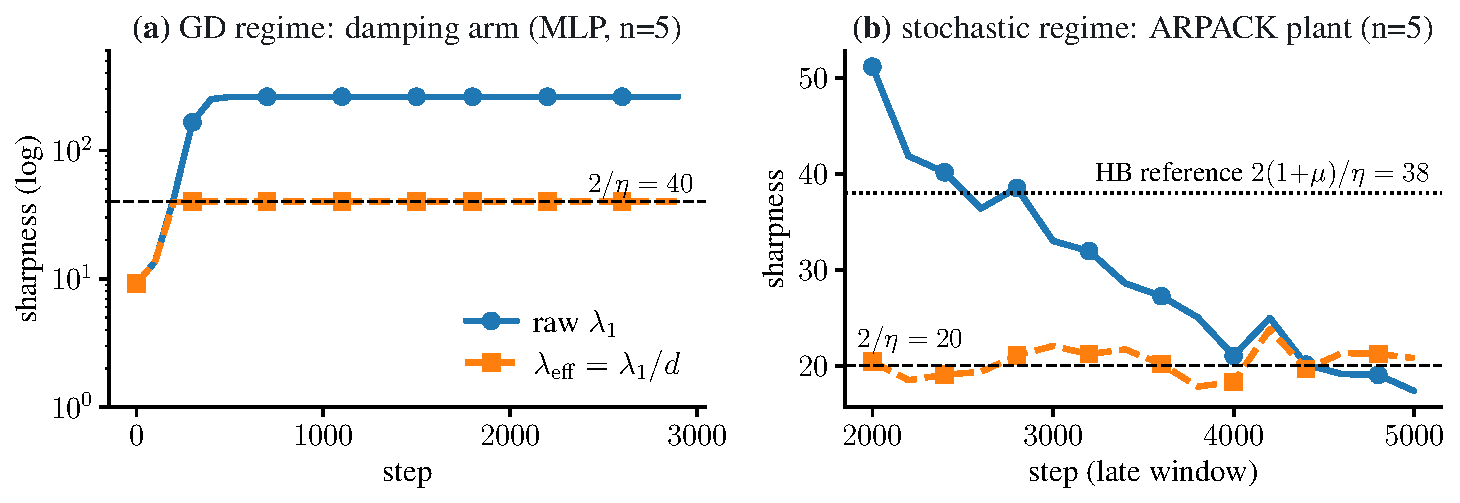
\includegraphics[width=0.95\linewidth]{34_precond_sharpness.pdf}
\caption{Control-law bookkeeping of the preconditioned sharpness
$\lambda_{\mathrm{eff}}$ (Corollary~\ref{cor:upward}) under the \emph{adaptive}
self-gating rule. \textbf{(a)} GD regime (MLP, accurate rank-1 damping,
$n{=}5$, seed-mean): the raw sensed $\hat\lambda_{1}$ escapes past
$2/\eta{=}40$ to ${\sim}\!262{\approx}6.6\cdot 2/\eta$ while
$\hat\lambda_{1}/d$ sits at $2/\eta$ throughout the climb (log scale).
This panel is \emph{definitional} whenever the clamp fires
($d=\hat\lambda_{1}/(2/\eta)$ by construction): it verifies the
control law's internal consistency, and the interventional test of the
$\lambda_{\mathrm{eff}}$ claim is the fixed-divisor control of
Fig.~\ref{fig:etad}. \textbf{(b)} Stochastic regime
(ResNet-18/CIFAR-100, accurate ARPACK-sensing damping arm, $n{=}5$,
late window): raw $\lambda_{1}$ (independent tol-$10^{-6}$ outcome
ARPACK; no statistically resolved difference from SGD) while $\lambda_{1}/d$ sits at
$20.40\pm0.65=(1.02\pm0.03)\cdot 2/\eta$, here a measurement-consistency
statement (independent outcome vs.\ stale sensing), not an identity; the
heavy-ball reference line at $38$ and the SGD raw level $29.2$ are shown for
contrast.}
\label{fig:precond}
\end{figure}

\begin{corollary}[rank-1 amplification descends below the threshold (sign-flip control)]
\label{cor:amplify}
Run the same fixed-point algebra of
the algebraic part of the restatement below at the opposite sign of the
edit: $\gamma=-\alpha<0$ (i.e.\ $g'=g+\alpha(g^{\top}u_{1})u_{1}$,
$\alpha>0$), with \textbf{A1}--\textbf{A3} otherwise unchanged. Every
sign-flip period-2 fixed point then satisfies
$y^{*}=\tfrac{2\gamma}{(1-\gamma)\eta}=-\tfrac{2\alpha}{(1+\alpha)\eta}<0$,
i.e.\ $S_{*}=2d/\eta$ with $d=\tfrac{1}{1+\alpha}\in(0,1)$:
\emph{$\lambda^{*}=2/((1+\alpha)\eta)<2/\eta$, and
$S_{*}\downarrow0$ monotonically as $\alpha\uparrow\infty$} (never below
$0$). The conditional $y$-contraction part of the restatement below becomes
$|\mu_{y}|<1$ iff $(1+\alpha)\eta^{2}\alpha_{\mathrm{ps}}<1$, \emph{harder} to satisfy as
$\alpha$ grows, unlike damping, where $\gamma\uparrow1$ makes it easier.
\emph{Experimentally confirmed} (\S\ref{sub:amp}): rank-1 amplification with
accurate warm-started sensing descends below the threshold at every tested $\alpha$, with
late-window equilibria monotone in $\alpha$, while the same sensing with
$\gamma>0$ escapes past $2/\eta$
(Lemma~\ref{prop:boundary}); the realized equilibria sit
below the naive $\lambda^{*}=2/((1{+}\alpha)\eta)$ values, consistent with
Corollary~\ref{cor:upward}'s direction-only disclaimer. (At ResNet-18
scale, rank-1 amplification shows no statistically resolved effect,
whereas increasing the amplified rank to $k{=}20$ and applying the
full-rank first-order correction both shift sharpness upward rather
than reproducing the full-batch descent
(\S\ref{sub:scale}), so the corollary's downward escape is specific
to the GD-regime dynamics.) The lemma's
negative statement is thereby \emph{sharpened, not contradicted}: what cannot
descend below the threshold is rank-1 \emph{damping} ($\gamma\in(0,1)$), not rank-1 actuation
in general.
\end{corollary}

\begin{remark}[partial multi-eigenvalue extension (separable case)]
\label{rem:separable}
If $H$ is separable, $H=\sum_{i}\lambda_{i}u_{i}u_{i}^{\top}$ with no
off-diagonal coupling, the Damian recurrence decouples into independent
$(x_{i},y_{i})$ pairs and Lemma~\ref{prop:boundary} applies
\emph{per direction}: damping any subset of eigenvectors leaves each undamped
direction's cap at $y_{i}^{*}=0$ or moves each damped direction to
$y_{i}^{*}>0$. The multi-sharp test (\S\ref{sec:control}) provides an
empirical check consistent with per-direction independence on one
non-separable landscape, the regime \citet{damian2023selfstab} leave
theoretically open. A general multi-eigenvalue extension remains open
(gap~\textbf{G1}).
\end{remark}

\paragraph{Connection to projection-based precedents.}
\citet{song2025bulk} project the SGD update onto the spectral ``bulk'' (removing
the top-$k$ eigenvector components) and report that sharpness grows unconstrained
while loss and accuracy are preserved. This is the $\gamma\!\to\!1$
($d\!\to\!\infty$) limit of our rank-1 damping: Corollary~\ref{cor:upward}'s
equilibrium $S_{*}=2d/\eta$ diverges as $d\!\to\!\infty$, so their observation
is regime~(ii) (cap removed) taken to its extreme: the unconstrained growth is
the predicted divergence of the orbit location itself, not a separate phenomenon.
Our partial-damping ($\gamma<1$) experiments diagnose the cap at finite
$S_{*}$; their full-projection ($\gamma=1$) removes it entirely. Their
``pseudo-alignment'' reading and our ``cap-removal'' reading describe the same
trajectory through different lenses; only the cap-removal lens predicts the
$\gamma$-dependent divergence quantitatively.

\begin{remark}[Connection to SAM]
\label{cor:sam}
SAM's update $\theta_{t+1}=\theta_{t}-\eta\nabla L(\theta_{t}+\rho\nabla L/\|\nabla L\|)$
does \emph{not} enter the rank-1 recurrence \eqref{eq:damped-x-formal}: expanding
to $O(\rho)$ \citep{andriushchenko2022sam}, its effective gradient is
$\nabla L^{\mathrm{SAM}}\approx(I+\tfrac{\rho}{\|g\|}H)g$, rescaling the top
direction by $1+\rho\lambda_{1}/\|g\|>1$ (curvature-amplifying), which lowers the
stability boundary SAM tracks to
$\lambda^{*}_{\mathrm{SAM}}=\tfrac{\|g\|}{2\rho}\bigl(\sqrt{1+\tfrac{8\rho}{\eta\|g\|}}-1\bigr)<2/\eta$
\citep{long2024sam}, i.e.\ $y^{*}_{\mathrm{SAM}}<0$. Rank-1 damping rescales the
top direction by $1/d<1$ (curvature-attenuating), raising the boundary to
$y^{*}>0$. This is the formal content of the attenuation-vs-amplification
dichotomy: the two edits move the EoS threshold in opposite directions
along the \emph{same} monotone $y^{*}(\gamma)$ of \eqref{eq:ystar}, and
reaching the sub-threshold region $y<0$ requires the amplifying sign. The
amplifying sign does \emph{not} have to be global: rank-1 amplification on the
top direction alone reaches $y^{*}<0$ (Corollary~\ref{cor:amplify}). At
first order, SAM contains a curvature-weighted correction whose
positive-curvature components have the amplifying sign; this motivates the
sign comparison with Corollary~\ref{cor:amplify}, but full SAM is not
identified with this linear amplification: \S\ref{sub:sammech} shows
that the finite re-query residual bundle carries the observed
endpoint difference along the tested ResNet interpolation.
\end{remark}

The assumptions above define the regime in which the reduced
recurrence is interpretable; we do not empirically certify each
assumption pointwise along every network trajectory. In particular,
spectral isolation, slow variation of the reduced coefficients, and
piecewise-constant sensing are modeling conditions rather than
measured invariants of the full network dynamics.

\paragraph{Gap inventory (2-D theorem $\to$ trajectory theorem).}
\begin{itemize}
  \item[\textbf{G1}] \emph{Multi-eigenvalue decoupling.} The lemma
        projects dynamics onto $(u_{1},\mathrm{rest})$; the multi-eigenvalue
        extension \citet{damian2023selfstab} defer (\S8.2) is open.
  \item[\textbf{G2}] \emph{Rotation singularity.} A1 fails at eigenvalue
        crossings $\lambda_{1}\leftrightarrow\lambda_{j^{*}}$, where $\nabla S$
        is singular; patching is open (empirically the trajectory crosses in
        $O(\eta^{-1})$ steps with the qualitative verdict intact).
  \item[\textbf{G3}] \emph{Time-varying $\gamma$.} A2 freezes $\gamma$; the
        extension to piecewise-constant $\gamma_{t}$ (refresh interval $N$) needs
        a perturbation analysis.
  \item[\textbf{G4}] \emph{Higher-order $x$-bounding.} Remark~\ref{rem:jacobian}'s
        fast-direction amplification is bounded by quartic-and-higher landscape
        terms the 2-D reduction omits.
  \item[\textbf{G5}] \emph{Sensing error.} A3 is ideal; with $\hat v$ at angle
        $\varphi$ to $u_{1}$ the effective damping is
        $\gamma_{\mathrm{eff}}=\gamma\cos^{2}\varphi$ and the lemma holds
        with $\gamma\to\gamma_{\mathrm{eff}}$.
\end{itemize}

\subsection{Two further controls confirm cap robustness}
\label{app:two-controls}

The lemma concerns damping the \emph{top} direction. Two further controls
test the symmetric direction and the effect of sensing lag; both confirm that
descent below the threshold did not occur for any single-direction \emph{attenuating} or
lagged edit we test (the amplifying sign is tested separately,
Corollary~\ref{cor:amplify}). The
empirical data for both live in \S\ref{sec:control} (Fig.~\ref{fig:c4lag});
here we state the structural content only.

\begin{corollary}[orthogonal damping leaves the cap intact]
\label{cor:orth}
The C4 edit $\Delta\theta=-\eta(g_{\parallel}+g_{\perp}/d)$ with
$g_{\parallel}=(g^{\top}u_{1})u_{1}$ preserves the gradient component along
$u_{1}$. Its $x$-recursion is therefore the undamped Damian map
$x_{t+1}=-(1+\eta y_{t})x_{t}$, whose period-2 fixed point is $y^{*}=0$. The
orthogonal damping rescales only the complement and does not enter the
top-direction dynamics. The cap holds for every $d$ because the $x$-recursion is the undamped Damian
map, whose sign-flip fixed point is $y^{*}=0$ \emph{regardless} of how the
$y$-drift coefficient is affected: the edit-induced correction to the drift is
odd in $x$ (zero mean per cycle) and its even remnant only renormalizes the
amplitude-setting $\beta$, which does not enter the cap location.
Experimentally confirmed in \S\ref{sec:control}
(Fig.~\ref{fig:c4lag}); the widening of per-seed variance at large $d$
reported there is a measured instance of gap~\textbf{G4}, where freezing the
complement weakens the higher-order $|x|$-bounding the 2-D reduction omits.
\end{corollary}

Together with Lemma~\ref{prop:boundary} (top-direction
damping $\Rightarrow$ $y^{*}>0$, upward escape) and Corollary~\ref{cor:orth}
(orthogonal damping $\Rightarrow$ $y^{*}=0$, cap intact), the verdict is
symmetric: damping either direction alone fails to achieve sub-threshold escape; descending
below requires the amplifying sign: global (Remark~\ref{cor:sam}) or
rank-1 local (Corollary~\ref{cor:amplify}).

\begin{observation}[short sensing lags preserve the response; the
gradient-direction proxy pins]
\label{obs:lagged}
The delayed-update sensor $\hat v_{k}=\Delta\theta_{t-k}/\|\cdot\|$ conflates
two distinct imperfections: \emph{lag}, and using the update (gradient)
direction rather than the eigenvector. Separating them shows that only the
second pins (\S\ref{sec:control}, Fig.~\ref{fig:c4lag}): the lagged-but-accurate
sensor $\hat v_{k}=\hat u(t{-}k)$ stays in regime~(ii), because $u_{1}$
rotates on the slow $O(1/\eta)$ timescale \citep{damian2023selfstab} and
$\hat u(t{-}k)\approx u_{1}(t)$ (we test only short lags $k\le3$). The lagged
update-direction sensor $\hat v_{k}=\Delta\theta_{t-k}\propto-g$, by contrast,
suffers a \emph{self-induced sensing failure}: the edit's own damping rotates
the update direction, the lagged $\hat v$ drifts off $u_{1}$, its Rayleigh
quotient collapses, the self-gating clamp sets $\gamma{=}0$, and the system
reduces to undamped Damian GD with $y^{*}=0$ (Remark~\ref{rem:regime-i}): the
operative cause is inaccuracy, not staleness.
\end{observation}
The cap is thus robust to the tested short sensing \emph{lags}
($k\le3$) but not to sensing \emph{inaccuracy}: only accurate top-direction
sensing achieves cap removal, and the failure of the delayed-update proxy is
attributable to sensing-direction inaccuracy rather than to these tested
lags.
(Without the self-gating clamp, a stale Rayleigh quotient flips $\gamma<0$ and
anti-damps to divergence: an optimizer pathology, not cap removal;
\S\ref{sec:control}.)


\section{The proxy ladder and monitor comparisons}
\label{app:proxy}
This appendix is supporting instrumentation for the control study of
\S\ref{sec:control} and \S\ref{sec:theory}: it characterizes the cheap
sharpness monitors used as diagnostics throughout, and delimits, via a
one-HVP warm-started comparator (\S\ref{sub:wscompare}), when the
gradient Rayleigh quotient is the right monitor for the regime at hand.

\subsection{Zero-compute (Tier-0) proxies are normalization-dependent and seed-unstable}
On plain nets, every layer's weight norm tracks $\lmax$ (mean Pearson
$0.65$--$0.71$ over $14$ runs: the main teacher--student run plus $13$
difficulty/lr/width sweeps), with the \emph{last-hidden} layer best (best
layer in $10/14$ runs), refining
\citet{li2022sharpness}. Under BatchNorm the correlation \emph{flips sign}
($-0.8$): BN renormalizes activations, decoupling $\|\mathbf{W}\|$ from
curvature; the affine scale $\gamma$ inherits the signal. However, multi-seed
($n=5$) the BN-$\gamma$ proxy is \textbf{unstable}: detrended
$+0.247\!\pm\!0.340$ (per-seed from $+0.55$ to $-0.05$), CI spanning zero. On
LayerNorm-based Transformers, zero-compute norms plateau: gradient norm
$\|\mathbf{g}\|$ is marginally best ($+0.52$ on both ViT and ConvNeXt) but only
$\sim\!0.08$ above $\|\gamma\|$/$\|W_{\mathrm{attn}}\|$ ($\sim\!0.44$), and
splitting attention from MLP weights does not help. (A $16$-point detrended
correlation can swing $\pm0.25$ across reasonable windows because $\|\gamma\|$
moves $<\!1\%$ while $\lmax$ swings $20\times$; dense sampling gives $+0.44$.)

\subsection{A single-HVP gradient Rayleigh quotient: a high-correlation trajectory monitor in the EoS regime}
The quantity $\lhatg=\mathbf{g}^{\!\top}\!H\mathbf{g}/\mathbf{g}^{\!\top}\!\mathbf{g}$
(one Hessian-vector product) is algebraically the critical sharpness
$\lambda_c$ on a quadratic \citep{kalra2026scalable} and a Rayleigh lower bound
on $\lmax$, tight iff $\mathbf{g}$ aligns with $v_{\mathrm{top}}$. Empirically on
the ResNet (Table~\ref{tab:proxy}, Fig.~\ref{fig:rayleigh}): detrended
$r=+0.898\!\pm\!0.141$ over the whole trajectory and $+0.981\!\pm\!0.030$ in the
EoS regime ($|\cos(\mathbf{g},v_{\mathrm{top}})|>0.7$), where the $\sim\!17\%$
relative gap is the expected Rayleigh lower-bound slack (the EoS-regime
alignment is higher, $|\cos|\!\to\!0.85$--$0.9$, giving $\cos^{2}\!\approx\!0.8$),
not measurement noise. This dominates every Tier-0 proxy and the BN-$\gamma$
baseline at $+0.247\!\pm\!0.34$. Cost: one HVP for the deployed monitor (vs
$\sim\!5$ HVPs for exact warm-started measurement \citealp{ramasinghe2026taming},
vs $5$--$6$ forward passes for the $\lambda_c$ line search
\citealp{kalra2026scalable}).

\begin{table}[!ht]
\centering\small
\caption{Single-HVP $\lhatg$ vs Tier-0 proxies on the ResNet ($n=5$ seeds).
Detrended Pearson $r$ with $\lmax$.}
\label{tab:proxy}
{\renewcommand{\arraystretch}{1.10}\RTableTopGap
\begin{tabular}{lcc}
\toprule
proxy & whole trajectory & EoS regime ($|\cos(\mathbf{g},v_{\mathrm{top}})|>0.7$) \\
\midrule
$\lhatg$ (1 HVP, gradient)      & $\mathbf{+0.898\!\pm\!0.141}$ & $\mathbf{+0.981\!\pm\!0.030}$ \\
$\lhatd$ (1 HVP, update)        & $+0.896\!\pm\!0.144$          & $+0.975\!\pm\!0.047$ (err $0.238\!\pm\!0.026$) \\
$\|\mathrm{BN}\,\gamma\|$ (0 HVP) & $+0.247\!\pm\!0.340$ (unstable) & --- \\
\bottomrule
\end{tabular}}
\end{table}

The Rayleigh bound $\lhatg\leq\lmax$ held at $248/248$ informative
measurement points across the $n{=}5$ monitor runs (the five exceptions
are the initialization step, where both quantities are ${\sim}10^{-2}$
and the reference reads noise), and two eigenvector-free candidates for a
deployment gate (thresholding $\lhatg$ against $2/\eta$, and a
self-referential saturation rule) failed to isolate the aligned regime
with useful precision, so none is claimed.


\subsection{The monitor probe is the gradient, not the update}
\label{sec:gvstd}
For $\lmax$ \emph{monitoring}, the raw gradient beats the momentum-smoothed
update: $|\cos(\mathbf{g},v_{\mathrm{top}})|=0.563\!\pm\!0.017 >
|\cos(\Delta\theta,v_{\mathrm{top}})|=0.511\!\pm\!0.024$,
and the EoS relative error of $\lhatg$ ($0.169\!\pm\!0.026$) is below that of
$\lhatd$ ($0.238\!\pm\!0.026$). The whole-trajectory
correlations of $\lhatg$ and $\lhatd$ are tied ($\sim\!0.90$): the distinction
shows up in alignment and EoS error, not in global correlation. Mechanistically,
the momentum buffer is an EMA of past mini-batch gradients whose directional
noise \emph{dilutes} alignment with $v_{\mathrm{top}}$. This bifurcates our use
from CDAT/Kalra: step-size \emph{tuning} wants the (preconditioned) update
direction; $\lmax$ \emph{monitoring} wants the raw gradient. This
distinction also limits the causal interpretation of the stochastic
intervention-strength analysis: our controller edits and energy
shares are defined on the instantaneous gradient, whereas the
optimizer state that determines the parameter displacement contains
accumulated momentum.

\subsection{A one-HVP warm-start comparator: when the quotient is the
right monitor}
\label{sub:wscompare}
The quotient's one-HVP cost is shared by a natural alternative: a
warm-started power-iteration tracker that carries its previous
eigenvector estimate forward and refines it with a single HVP per
measurement \citep{ramasinghe2026taming}. We compared the two estimators
at identical cost and measurement cadence (one measurement per $50$
steps; ground truth = warm-started power iteration / ARPACK $\lmax$; EoS
gate $|\cos(\mathbf{g},v_{\mathrm{top}})|>0.7$) on two families: (A) the
MLP teacher--student testbed (full-batch GD, offline exact-HVP
reconstruction, $n{=}5$ seeds, $59$ points per seed) and (B) the
CIFAR-10 PreAct-ResNet ($0.175$M parameters, BatchNorm + momentum,
mini-batch; online tracker, $n{=}5$ seeds, $51$ points per seed;
Table~\ref{tab:wscompare}).

The regime contrast is the point. In the full-batch slow-drift family
(A) the tracker dominates at equal cost: it rides the warm-started
eigenvector (mean $|\cos(v_{\mathrm{ws}},v_{\mathrm{top}})|=0.915$,
vs.\ $|\cos(\mathbf{g},v_{\mathrm{top}})|=0.427$ for the gradient) and
its median level error is ${\sim}0.03$ where the quotient's Rayleigh
slack is ${\sim}1$: outside the EoS window the gradient is nearly
orthogonal to $v_{\mathrm{top}}$, so the quotient reads the spectral
bulk. Under mini-batch churn the roles reverse: between $50$-step
measurements the BatchNorm parameters and the iterate move enough that
the carried vector goes stale (mean overlap $0.582$), and the tracker
decorrelates ($0.118\!\pm\!0.139$ overall; $-0.061\!\pm\!0.272$ in the
EoS window) exactly where the quotient is strongest
($0.987\!\pm\!0.008$). The quotient's value is therefore not universal
cost superiority (at matched cost the tracker wins in slow-drift
regimes) but its gradient-coupled semantics and EoS-regime coverage: it
monitors the direction the optimizer actually uses, precisely in the
regime this paper studies. Ground truth costs $3.9$ HVPs per measurement
in family A and $13.8$ in family B.\footnote{Scope caveats: both
families are toy-scale (an MLP teacher--student testbed and a $0.175$M
PreAct-ResNet); the cadence is one measurement per $50$ steps, not
per-step; the MLP comparator uses offline exact-HVP reconstruction,
validated by a loss gate $\le 2\times10^{-7}$ and agreement of the
reconstructed $\lhatg$ with its online value to $\le 3.5\times10^{-5}$;
and $4/295$ MLP tracker estimates are marginally negative (isolated
steps ${\sim}850$--$1050$ on seeds 1--3, minimum $-0.075$), which we
report as-is rather than clip.}

\begin{figure}[!ht]
\centering
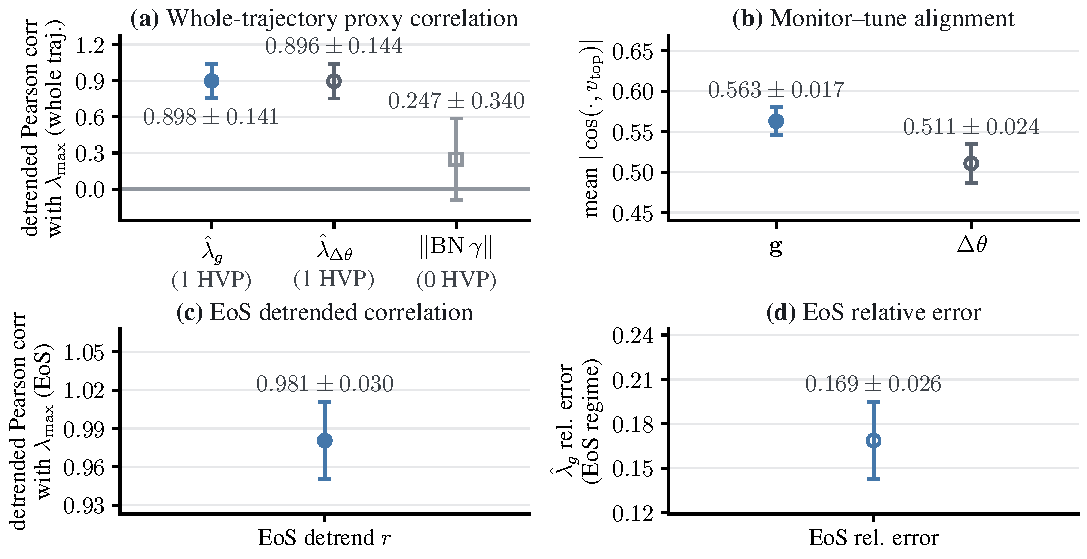
\includegraphics[width=0.92\linewidth]{fig1_rayleigh_monitor_ci.pdf}
\caption{Gradient Rayleigh-quotient monitoring on the ResNet ($n=5$ seeds).
\textbf{(a)}~Whole-trajectory detrended Pearson correlation with $\lmax$;
\textbf{(b)}~mean absolute alignment with $v_{\mathrm{top}}$;
\textbf{(c)}~EoS-window detrended correlation; \textbf{(d)}~EoS relative
level error. Bars show the across-seed mean$\pm 95\%$ CI. The one-HVP
gradient Rayleigh quotient $\lhatg$ is robust in the EoS window, the
Tier-0 $\|\mathrm{BN}\,\gamma\|$ proxy is seed-unstable, and $\mathbf{g}$
aligns with $v_{\mathrm{top}}$ better than $\Delta\theta$.}
\label{fig:rayleigh}
\end{figure}

\begin{table}[!ht]
\centering\footnotesize
\setlength{\tabcolsep}{4pt}
\caption{One-HVP warm-started power-iteration tracker
($\hat\lambda_{\mathrm{ws}}$) vs.\ the gradient Rayleigh quotient
$\lhatg$ at identical cost and cadence (measurement every $50$ steps;
ground truth = warm-started power iteration / ARPACK $\lmax$; EoS gate
$|\cos(\mathbf{g},v_{\mathrm{top}})|>0.7$; mean$\pm 95\%$ CI over $n{=}5$
seeds; rel.\ err.\ = median relative level error; ms = wall-clock per
measurement; early = pre-EoS window, not defined for the online family
B).}
\label{tab:wscompare}
{\renewcommand{\arraystretch}{1.10}\RTableTopGap
\begin{tabular}{llccccc}
\toprule
family & estimator & Pearson & early & EoS & rel.\ err.\ (med.) & ms \\
\midrule
A: MLP full-batch & $\hat\lambda_{\mathrm{ws}}$ & $0.981\!\pm\!0.004$ & $0.979\!\pm\!0.008$ & $0.976\!\pm\!0.033$ & $0.027\!\pm\!0.014$ & $5.8$ \\
A: MLP full-batch & $\lhatg$ & $0.537\!\pm\!0.070$ & $0.464\!\pm\!0.237$ & $0.913\!\pm\!0.121$ & $0.982\!\pm\!0.001$ & $6.0$ \\
\addlinespace[2pt]
B: PreAct-ResNet & $\hat\lambda_{\mathrm{ws}}$ & $0.118\!\pm\!0.139$ & --- & $-0.061\!\pm\!0.272$ & $0.321\!\pm\!0.026$ & $29.8$ \\
B: PreAct-ResNet & $\lhatg$ & $0.919\!\pm\!0.067$ & --- & $0.987\!\pm\!0.008$ & $0.344\!\pm\!0.033$ & $33.0$ \\
\bottomrule
\end{tabular}}
\end{table}

\FloatBarrier

\section{Robustness controls: full protocols and results}
\label{app:robust}

\subsection{Protocol map and reading guide}
\label{app:protocolmap}
The empirical logic is deliberately staged.
Section~\ref{sec:control} asks only whether a known orbit-location
prediction survives a feedback-free full-batch intervention;
Section~\ref{sec:stochastic} then drops the reduced-model
interpretation and treats the stochastic experiments as
protocol-specific intervention outcomes; Section~\ref{sub:sammech}
uses SAM only as a contrasting control family, not identified with
the full-batch amplification mechanism.

\textbf{Protocol map.}
The full-batch fixed-divisor experiments use unconditional fixed
$d{>}1$ attenuation with accurate warm-started sensing. The canonical
stochastic rank-1 result is reported for both the legacy gated
sensor and corrected ARPACK sensing; mechanistic conclusions use the
corrected result. The wider stochastic rank experiments use the
no-floor raw-divisor signed rescaling of \S\ref{sub:inertness}. The
clamp-free control of \S\ref{sub:bridge} is a separate bridge
experiment, not unconditional damping. SAM/linSAM experiments use
current-minibatch first-order or re-query gradients, not the
eigenspace-rescaling rule.

\subsection{Proxy-driven norm caps (C1, C2)}
\label{app:normcaps}
\textbf{(C1) Control on a plain net: weight-norm cap.} Project
$\|\mathbf{W}_{\mathrm{lh}}\|$ onto a tight ball when it exceeds budget
$1.01\!\cdot\!\|\mathbf{W}_{\mathrm{lh}}\|_{\mathrm{init}}$. The projection fires
on $\sim\!750$ of $3000$ steps (per-seed $745/751/746/745/723$, $n\!=\!5$), yet
$\lraw^{\mathrm{final}}=40.26\!\pm\!0.43=2/\eta$ (no escape); the peak is not
reduced within seed-noise.

\textbf{(C2) Control on a BN net: $\gamma$-cap.} Project all BN-$\gamma$ onto
$1.02\!\cdot\!\|\gamma_{\mathrm{init}}\|$. $\lraw^{\mathrm{final}}=81.6\!\pm\!19.2$
vs baseline $73.0\!\pm\!12.9$ (no escape; accuracy slightly worse, $0.754$ vs
$0.768$).

\subsection{Cap robustness: orthogonal damping and sensing lag}
\label{sub:caprobust}
\textbf{Damping the orthogonal complement also fails (C4: cap-robust).}
The rank-1 edit damps the \emph{top} direction; the symmetric control damps
\emph{everything else}, $\Delta\theta=-\eta(g_{\parallel}+g_{\perp}/d)$, keeping
the top-direction gradient intact (Corollary~\ref{cor:orth}). Sweeping
$d\in\{1,1.5,2,4,8\}$ ($n{=}5$, MLP full-batch), \lraw\ pins at $2/\eta\approx40$
for every $d$ ($40.2,40.3,38.9,43.4,40.1$; $0/5$ seeds diverge). The orthogonal
damping slows convergence (final loss $0.11\!\to\!0.59$ as $d\!\to\!8$) and
shrinks the along-$u_{1}$ oscillation ($|x_{t}|$ $0.18\!\to\!0.03$), but the
top-direction self-stabilization is untouched, exactly as the 2-D reduction
predicts ($g_{\parallel}$ preserved $\Rightarrow$ the $x$-recursion is the
undamped Damian map $\Rightarrow$ $y^{*}=0$). At $d\ge4$ the per-seed spread
widens sharply (CI $\pm9$ at $d{=}4$ vs $\pm0.3$ at $d\le1.5$, $\pm1.7$ at
$d{=}2$): freezing the
complement removes directions that help bound the $u_{1}$ oscillation, and the
the constant-$\alpha$ 2-D reduction loses precision: a measured instance of
gap~\textbf{G4}, neither a descent below the threshold nor an upward escape ($0/5$ diverge at every $d$). With
the rank-1 result (top damping
$\Rightarrow$ escape past $2/\eta$), the two single-direction controls fail
by \emph{opposite} mechanisms: one removes the cap upward, the other leaves it in
place. Neither descends below the threshold.

\textbf{Short sensing lags ($k\le3$) preserve the response; the failure of
the delayed-update proxy is attributable to sensing-direction inaccuracy
rather than to these tested lags.}
The delayed-update sensor $\hat v_{k}=\Delta\theta_{t-k}/\|\cdot\|$ conflates
lag with using the update (gradient) direction rather than the eigenvector.
Separating them ($n{=}5$, MLP): the lagged-but-\emph{accurate} sensor
$\hat v_{k}=\hat u(t{-}k)$ escapes upward to the \S\ref{sub:rank1} escape value
for $k{=}1,2,3$, numerically identical to $k{=}0$; $u_{1}$ rotates on the
slow $O(1/\eta)$ timescale, so $\hat u(t{-}k)\approx u_{1}(t)$ and the cap is
still removed (Observation~\ref{obs:lagged}). The lagged \emph{update-direction}
sensor $\hat v_{k}=\Delta\theta_{t-k}\propto-g$ pins at $2/\eta$ for
$k{=}1,2,3$ ($40.10\pm0.13,40.03\pm0.02,40.03\pm0.03$): the operative cause is
a \emph{self-induced sensing failure}, not staleness: the optimizer's own damping
rotates the update direction off $u_{1}$ and disengages the edit
(Remark~\ref{rem:regime-i}; reduced-model account in \S\ref{sec:theory},
Fig.~\ref{fig:c4lag}). With \emph{free lagged} $\hat v=\Delta\theta_{t-1}/\|\cdot\|$
($|\cos(\Delta\theta,v_{\mathrm{top}})|\!\to\!0.998$,
\citealp{damian2023selfstab}), $\lraw^{\mathrm{final}}=40.12\pm0.12=2/\eta$:
the lagged $\hat v$ imperfectly cancels $\mathbf{g}_{\parallel}$, the
period-2 oscillation persists, and the cap holds
(Claim~\ref{clm:rank1}, regime~i; Fig.~\ref{fig:control}). (Without the clamp, the stale
Rayleigh quotient flips $\gamma<0$ and \emph{anti-damps}: a divergence we
observe at $k{=}1$, step $\sim\!540$, an optimizer pathology.) The cap is thus
preserved under the tested short lags ($k\le3$); the delayed-update proxy's
failure is attributable to sensing-direction inaccuracy rather than to these
tested lags.

\begin{figure}[!ht]
\centering
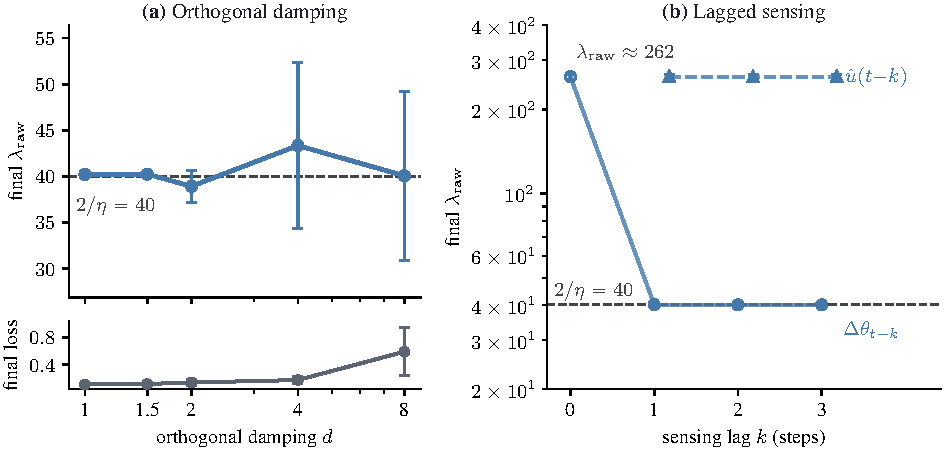
\includegraphics[width=0.95\linewidth]{31_c4_lagged_controls.pdf}
\caption{Two further controls on the MLP full-batch setup ($n{=}5$ seeds).
\textbf{(a)} Orthogonal damping (C4): \lraw\ pins at $2/\eta\approx40$ for every
tested $d\in\{1,1.5,2,4,8\}$ ($0/5$ diverge; loss rises $0.11\!\to\!0.59$, lower strip);
damping the complement does not touch the top-direction cap
(Corollary~\ref{cor:orth}). In (a), markers show across-seed means and
error bars 95\% CIs of the final-step \lraw\ ($n{=}5$). \textbf{(b)} Sensing lag vs.\ inaccuracy: the
lagged-but-accurate sensor $\hat u(t{-}k)$ escapes upward to $261.8\pm5.4$
($\triangle$), identical to $k{=}0$; the lagged update-direction sensor
$\Delta\theta_{t-k}$ pins at $2/\eta$ ($\circ$). Short lags ($k\le3$)
preserve the response; the
gradient-direction proxy, not staleness, pins (Observation~\ref{obs:lagged}).}
\label{fig:c4lag}
\end{figure}

\subsection{Clamp-free bridge: the null is not a clamp artifact}
\label{sub:bridge}
\textbf{Removing the self-gating clamp changes nothing (clamp-free C3).} The
X-SAM projector ablation (\S\ref{sub:sam}) revealed a potential confound in
the clamp design: the clamped X-SAM projector variant fired its rank-1 correction on $0\%$ of
steps where the matched-step (unclamped) one fires every step: the
$\max(\cdot,1)$ clamp can manufacture dormancy. The stochastic-regime
rank-1 arm uses
the \emph{same} clamp and showed no statistically resolved difference
from SGD partly through this viewpoint (it fired
on $\le\!4\%$ of steps, $\approx$ SGD), so that null could be
attributed to the clamp rather than the landscape. We
bridge this with a \emph{clamp-free} arm on the same CIFAR-100/ResNet-18
setup, deterministic CUDA, $n{=}5$ seeds (\texttt{-{}-no-clamp}): no
$\max(\cdot,1)$ gate, every direction fires every step (fired fraction
$100\%$), the raw divisor $d=\hat\lambda/\lambda_{\mathrm{targ}}$ allowed
below $1$.

\emph{What ``clamp-free'' edits} (Algorithm~\ref{alg:rank1}, clamp-free
branch). The semantics must be stated precisely: this
is \emph{not} an ``always damp'' arm. With $\alpha=\langle
\mathbf{g},\hat v\rangle$ the $\hat v$-component of the gradient, the edit is
$\mathbf{g}\mapsto\mathbf{g}-f\,\alpha\,\hat v$ with $f=1-1/d$ \emph{clipped
to} $[-1,1)$. When $\hat\lambda>\lambda_{\mathrm{targ}}$ ($d>1$), $f\in(0,1)$
and the edit damps, leaving $\alpha/d$. When
$\hat\lambda<\lambda_{\mathrm{targ}}$ ($d<1$), the factor flips sign
($f<0$): instead of opposing the $\hat v$-component, the edit reinforces
it: bounded sign-flip anti-damping. The clip keeps the edit magnitude at
most $|\alpha|$ and the post-edit $\hat v$-component at most $2|\alpha|$, so
the anti-damping is bounded and cannot explode. This bound is exactly what
separates the bridge from the un-clipped lagged variant of
\S\ref{sub:caprobust} (Fig.~\ref{fig:c4lag}), whose raw factor
($\gamma\!\to\!-\infty$ as the stale Rayleigh quotient collapses) anti-damped
into divergence at $k{=}1$, step $\sim\!540$: there the sign flip was
unbounded and diverged, here it is clipped: the two clamp-free statements
are consistent, and it is the bound, not the gate, that separates them.

\emph{No upward escape without the clamp.} We compare four arms under one
deterministic driver (\mbox{Table~\ref{tab:bridge}}), reporting the late-window
(step $\geq 2000$) single-HVP gradient Rayleigh quotient $\lhatg$ on the
deterministic 512-sample eval batch ($n{=}5$ seeds, mean$\pm 95\%$ CI). At
this stage the power-iteration $\lmax$ estimate was not yet trustworthy (the
false convergence later diagnosed in \S\ref{sub:scale}), so we report the
deterministic per-model proxy $\lhatg$, a lower bound on $\lmax$
(\S\ref{sec:discuss}), and keep all comparisons within-protocol.

\begin{table}[!ht]
\centering\small
\caption{Clamp-free bridge, CIFAR-100/ResNet-18, deterministic CUDA ($n{=}5$
seeds): late-window (step $\geq 2000$) $\lhatg$ mean$\pm 95\%$ CI, and the
fired fraction of the rank-1 correction. \textbf{Within-protocol comparison
only}: $\lhatg$ is a single-HVP lower-bound proxy on a fixed eval batch and
its absolute scale (13--18) is \emph{not} comparable to the ARPACK \lref\
scale (22--29) of the stochastic-regime control in \S\ref{sub:scale}.}
\label{tab:bridge}
{\renewcommand{\arraystretch}{1.10}\RTableTopGap
\begin{tabular}{lcc}
\toprule
arm & late $\lhatg$ & fire\% \\
\midrule
SGD & $18.73\pm1.29$ & --- \\
rank-1 (clamped C3) & $18.13\pm1.47$ & $4$ \\
\textbf{rank-1 (clamp-free C3)} & $\mathbf{17.14\pm1.21}$ & $100$ \\
SAM & $12.91\pm0.59$ & --- \\
\bottomrule
\end{tabular}}
\end{table}

The clamp-free arm does \emph{not} escape upward (Fig.~\ref{fig:bridge}): its
differences are $\Delta=-1.59$ vs.\ SGD and $-0.99$ vs.\ the clamped
arm, both well inside the $\sim\!1.5$-unit CIs, nowhere near the
upward escape of the accurate-$v_{\mathrm{top}}$ arm on the
full-batch MLP (the \S\ref{sub:rank1} escape value; Fig.~\ref{fig:rankk}). The unresolved rank-1
outcome is therefore robust to the clamp at this tested operating point: with the gate
removed and the correction firing every step, sharpness still shows no
statistically resolved difference from SGD. (The clamp-free arm does sit $\sim\!1.6$ below
SGD, the direction Duan et al.\ predict \citep{duan2026xsam}, but well
inside the CI and far smaller than SAM's $-5.8$; the no-resolved-contribution
verdict stands.) The same driver re-validates the deterministic
three-way: SAM ($12.91\pm0.59$) lies below both rank-1 arms
(paired $\Delta$ vs.\ SGD $-5.8$ above), so the stochastic-regime ordering of \S\ref{sub:scale} survives
the stricter determinism standard introduced by the X-SAM projector ablation.

\emph{Robustness of the null.} The two residual
suspicious readings of the stochastic-regime rank-1 result, clamp artifact and
dormant sensor, are excluded independently: the null survives
with the clamp removed \emph{and} with the sensor fixed. The ARPACK-sensing
arm of \S\ref{sub:scale} fires at full force (no clamp floor, refreshed
$v_{\mathrm{top}}$ every $N{=}20$ steps) yet still shows no statistically
resolved sharpness reduction relative to SGD at this tested operating point.

\begin{figure}[!htbp]
\centering
\IfFileExists{../figures/32_bridge_clampfree_c3.pdf}{%
  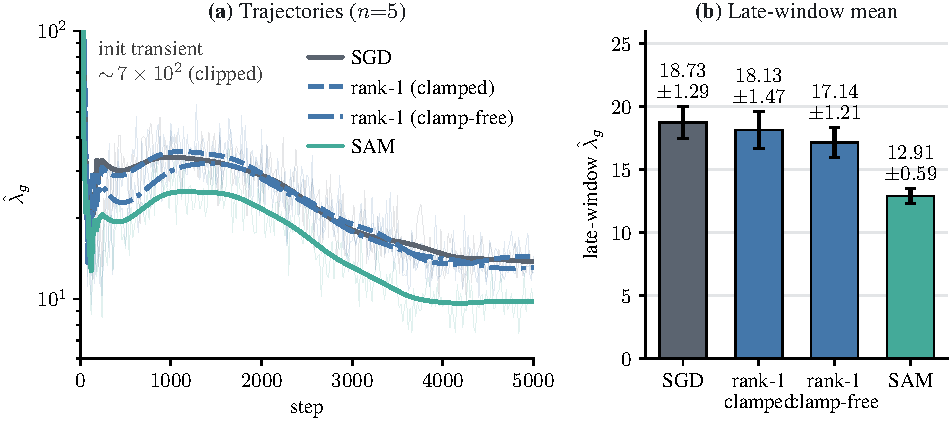
\includegraphics[width=0.92\linewidth]{32_bridge_clampfree_c3.pdf}}{}
\caption{Clamp-free bridge (deterministic CUDA, $n{=}5$ seeds): late-window
$\lhatg$ of SGD, clamped rank-1, clamp-free rank-1, and SAM:
(a) cross-seed mean trajectories Gaussian-smoothed in log space for display
(faint thin lines: unsmoothed means; the two-sample init transient is left
unsmoothed); (b) late-window mean$\pm 95\%$ CI (arms
distinguished by linestyle and hue, so the separation survives grayscale
printing). The clamp-free arm fires every step
yet stays within CI of SGD and of the clamped arm (no upward escape, no clamp
artifact) while SAM sits below them.}
\label{fig:bridge}
\end{figure}

\subsection{Sign-flip control: table and algorithm}
\label{app:ampdetails}

\textbf{Fixed-divisor grid, round 13 (Fig.~\ref{fig:etad};
\S\ref{sub:fixedd}).} Protocol: the \S\ref{sec:setup} tanh MLP
testbed (teacher--student synthetic, $n{=}1024$, dim $20$, student
$[256,256]$), full-batch GD, data seed $1$, model seeds $0$--$4$.
All $18$ cells of the unified round share one
CPU backend (float32, torch $2.9.1$, $8$ threads; $n{=}5$ seeds,
$3000$ steps; late window step $\geq1500$). Seven cells settle onto
the predicted orbit ($\eta{=}0.025$: ratios
$0.973/0.990/0.971$ at $d{=}1.25/1.5/2$; $\eta{=}0.05$:
$0.957/0.969/0.956/0.975$ at $d{=}1.25/1.5/2/6.5$). At $\eta{=}0.05$,
$d{=}6.5$ survives $3/5$ at ratio $0.975$, consistent with the
earlier GPU round ($3/5$, $0.997$; its single-$\eta$ levels
$47.9/59.2/74.7/259.3$ against $50/60/80/260$, ratios
$0.96/0.99/0.93/1.00$, agree within a few percent). Two $\eta{=}0.025$
cells survive off the identity: $d{=}2.5$ is intermittent (ratio
$0.592$; per-seed late means $100$--$150$), and $d{=}6.5$ sits at
$\lraw\approx258$ (per-seed $244$--$269$, sd $9$), an
$\eta$-independent saturation level coinciding with the
$\eta{=}0.05$, $d{=}6.5$ survivors' absolute level ($243$--$260$) and
with the rank-1 damping escape ceiling $261.8\pm5.4$
(\S\ref{sub:rank1}); we read it as a ceiling on the damped escape set
by the higher-order dynamics, not as a slow approach to $2d/\eta=520$.
All remaining cells diverge ($\eta{=}0.1$: $0/5$ throughout;
$\eta{=}0.05$, $d\in\{2.5,3\}$: $0/5$; $\eta{=}0.025$, $d{=}3$: $0/5$).

\emph{Round-13 reproducibility.} Relative to the previous CPU round,
interior cells reproduce to $\le1\%$ in the late-window mean, while
boundary (knife-edge) cells swing in survivor count and are not
bit-reproducible: CPU reduction order matters exactly at the
divergence boundary ($\eta{=}0.05$, $d{=}2$: $2/5$ here vs.\ $3/5$
previously). The paper uses only this unified round. We therefore do
not use survivor counts in these marginal cells as quantitative
evidence for a universal basin boundary; their role is only to show
that orbit survival is distinct from orbit location.

\textbf{Delayed-onset control (\S\ref{sub:fixedd}).} The fixed-$d$
survival grid is shown in Fig.~\ref{fig:etad}b. To isolate whether
the failures are caused by intervening too early, per seed, the
adaptive arm ran to its measured natural gate-opening step
$T_{\mathrm{gate}}$ (seeds $0$--$4$: $200/194/188/195/206$; mean
$196.6$), then switched to fixed $d\in\{2.5,3\}$ from exactly that
step: $0/5$ survive at both $d$ (divergence in every seed), while
the adaptive reference is $5/5$ stable from the same state (late
$\bar\lambda=258.2$, $\eta\bar\lambda/2=6.46\approx d{=}6.5$).

For the sign-flip amplification control of \S\ref{sub:rank1}, two
qualifications matter: (i) the amplified
equilibrium is \emph{intermittent}, not a clean pin: \lraw\ swings
between deep dips (${\sim}0$--$2$) and transient spikes
(${\sim}43$--$47$) on a ${\sim}500$-step scale, with window means tight
across seeds (per-seed $29.56$--$30.69$ at $\alpha{=}0.25$), consistent
with the arm's harder conditional $y$-contraction as $\alpha$ grows; and
(ii) the escape does not trade optimization for sharpness: minimum
losses match GD's ($0.092$--$0.095$ vs.\ $0.092$), though final losses
run modestly higher under the intermittency
($0.126\!\pm\!0.009\,/\,0.133\!\pm\!0.028\,/\,0.197\!\pm\!0.115$).

\FloatBarrier

\begin{table}[!ht]
\centering\small\setlength{\tabcolsep}{4pt}
\caption{Sign-flip control on the MLP full-batch setup ($n{=}5$ seeds):
late-window (step $\geq 1500$) \lraw, mean$\pm 95\%$ CI, and the fraction
of measurement steps below $2/\eta{=}40$. The 2-D reduction
(Corollary~\ref{cor:amplify}) predicts equilibria
$\lambda^{*}=2/((1{+}\alpha)\eta)$ for the amplifying arms: direction and
monotonicity, not magnitude (Corollary~\ref{cor:upward}).}
\label{tab:amp}
{\renewcommand{\arraystretch}{1.12}\RTableTopGap\RTableDenseRules
\begin{tabular}{lccc}
\toprule
arm & late \lraw\ & predicted $\lambda^{*}$ & frac${<}2/\eta$ \\
\midrule
GD                        & $37.49\!\pm\!1.76$ (final $39.92\!\pm\!0.40$) & $40$ (pin) & $0.56\!\pm\!0.32$ \\
rank-1 damping (accurate, full batch) & $261.8\!\pm\!5.4$  & --- (upward escape) & $0.00$ \\
SAM (full perturbed-point update) & $21.52\!\pm\!1.01$ & --- & $1.00$ \\
\midrule
rank-1 amp, $\alpha{=}0.25$ & $30.14\!\pm\!0.50$ & $32.0$ & $0.88\!\pm\!0.04$ \\
rank-1 amp, $\alpha{=}0.5$  & $22.45\!\pm\!1.27$ & $26.7$ & $0.97\!\pm\!0.07$ \\
rank-1 amp, $\alpha{=}1$    & $14.25\!\pm\!2.74$ & $20.0$ & $0.97\!\pm\!0.05$ \\
\bottomrule
\end{tabular}}
\end{table}

The magnitude gap grows monotonically with the edit strength
($-5.8\%/-15.9\%/-28.8\%$ at $\alpha=0.25/0.5/1$), consistent with the
weak-edit locality of the 2-D reduction rather than a sign error in the
fixed-point algebra: the reduction freezes
$(\alpha_{\mathrm{ps}},\beta,\lambda_{1})$ at the undamped operating point, and the
predicted orbit's displacement from that point grows with $\alpha$. Two
observations support this reading: at the weakest edit the gap is within the
realization offset the \emph{undamped} arm itself shows in the same window
(GD $37.49$ vs.\ the pin $40$), and the documented intermittency (deep
sub-threshold dips, spikes capped just above threshold, CI widening with
$\alpha$ as the conditional $y$-contraction tightens) is the orbit-level
signature of the $x$-odd correction terms the constant-coefficient reduction
omits (size $\propto\alpha$; Appendix~\ref{app:theory}), whose asymmetric
time-average sits below the sign-flip value. Both vanish in the weak-edit
limit $\alpha\to0$, where the prediction reduces to the undamped pin.
A fresh six-point grid run in a single session
($\alpha\in\{0.05,0.1,0.2,0.25,0.5,1\}$; $n{=}5$ seeds; late-window means
$37.5/33.5/31.7/28.6/23.9/15.2$ against predictions
$38.1/36.4/33.3/32.0/26.7/20.0$) verifies the weak-edit limit directly: the
realized-to-predicted gap at $\alpha=0.05$ is $-1.5\%$, within the
in-session undamped arm's own realization offset ($39.5$ vs.\ the pin
$40$, $-1.2\%$), and its magnitude grows with the edit strength
($-7.9/-5.1/-10.7/-10.2\%$ in the interior, $-23.8\%$ at $\alpha=1$).
This fresh grid is an independent validation run; Fig.~\ref{fig:amp} and
Table~\ref{tab:amp} report the original sign-flip run.

\begin{figure}[!htbp]
\centering
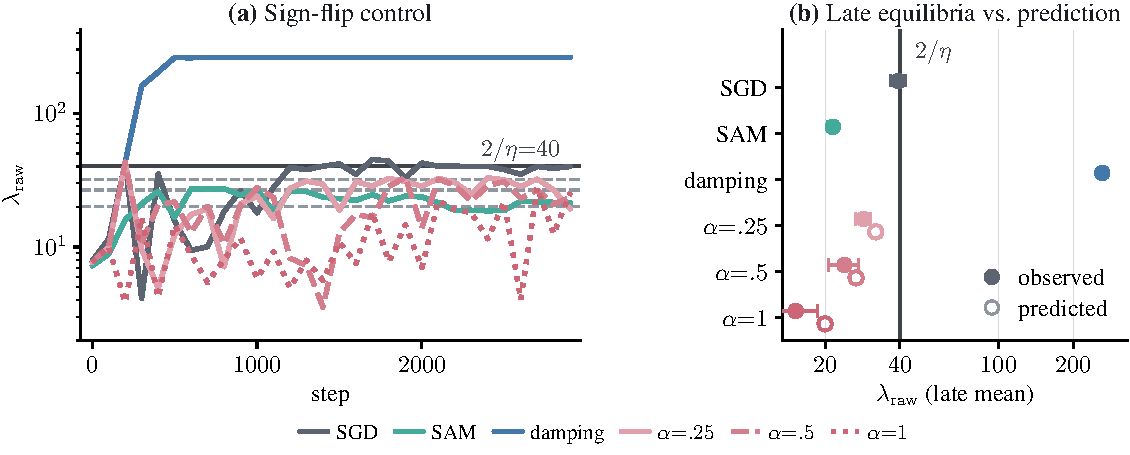
\includegraphics[width=0.95\linewidth]{33_rank1_amplify.pdf}
\caption{Sign-flip control on the MLP full-batch setup ($n{=}5$ seeds,
using the accurate-sensing MLP protocol of \S\ref{sub:rank1} and
Table~\ref{tab:amp}). \textbf{(a)} \lraw\ trajectories
(bold seed-mean): the attenuating rank-1 damping edit (accurate sensing)
escapes past $2/\eta{=}40$ to ${\sim}262$, while the sign-flipped
amplifying arms at $\alpha\in\{0.25,0.5,1\}$ descend below $2/\eta$ with
equilibria monotone in $\alpha$; SGD pins at $2/\eta$, and SAM descends below it.
\textbf{(b)} Late-window (step $\geq 1500$) mean$\pm 95\%$ CI against the
2-D prediction $\lambda^{*}=2/((1{+}\alpha)\eta)$ (thin gray dashed lines): the sign and
monotonicity match, while the realized equilibria sit below the naive fixed-point
values (direction-only, Corollary~\ref{cor:upward}).}
\label{fig:amp}
\end{figure}

\begin{algorithm}[!ht]
\caption{Rank-1 gradient edit (C3), the clamp-free bridge, and the
fixed-divisor interventional control}
\label{alg:rank1}
\begin{algorithmic}[1]
\Require step size $\eta$, gradient $\mathbf{g}=\nabla L(\theta)$, unit
$\hat v$ (free-lagged, power-iterated, or ARPACK-sensed), target
$\lambda_{\mathrm{targ}}{=}2/\eta$, variant $\in\{\text{clamped},
\text{clamp-free},\text{fixed-}d\}$
\State $\alpha \gets \langle \mathbf{g},\hat v\rangle$;\quad
       $\mathbf{g}_{\perp} \gets \mathbf{g}-\alpha\,\hat v$
       \Comment{split $\mathbf{g}$ along $\hat v$}
\State $\hat\lambda \gets \hat v^{\!\top}H\hat v$
       \Comment{one Hessian-vector product}
\State $d \gets \hat\lambda/\lambda_{\mathrm{targ}}$
\If{variant $=$ clamped (default C3)}
  \State $d \gets \max(d,\,1)$
         \Comment{self-gating clamp: fire only above target}
  \State $\tilde{\mathbf{g}} \gets \mathbf{g}_{\perp}+\alpha\,\hat v/d$
\ElsIf{variant $=$ fixed-$d$ (interventional control, \S\ref{sec:theory})}
  \State $d \gets d_{\mathrm{fix}}$ (constant)
         \Comment{no $\hat\lambda$ feedback: tests $\lambda_{\rm eq}{=}2d/\eta$}
  \State $\tilde{\mathbf{g}} \gets \mathbf{g}_{\perp}+\alpha\,\hat v/d$
\ElsIf{variant $=$ clamp-free}
  \State $f \gets \mathrm{clip}(1-1/d,\,-1,\,1)$
         \Comment{bounded sign-flip anti-damping below target}
  \State $\tilde{\mathbf{g}} \gets \mathbf{g}_{\perp}+(1-f)\,\alpha\,\hat v$
\EndIf
\State $\theta \gets \theta-\eta\,\tilde{\mathbf{g}}$
\State \Return $\theta$
\end{algorithmic}
\end{algorithm}

\subsection{Multi-sharp landscape test}
\label{app:multisharp}

Damping only $u_{1}$ lets $u_{1}$ escape upward while $\lambda_{2}$ stays pinned ($40.1\!\to\!65.2$, seed~0); here $k$ matters: $k{=}1\!:\!64.0<k{=}2\!:\!75.2\approx k{=}5\!:\!77.4$, each removed cap escaping independently. Figure~\ref{fig:multisharp} summarizes the final levels and the two-eigenvalue trajectories for this multi-sharp control.

\begin{figure}[!t]
\centering
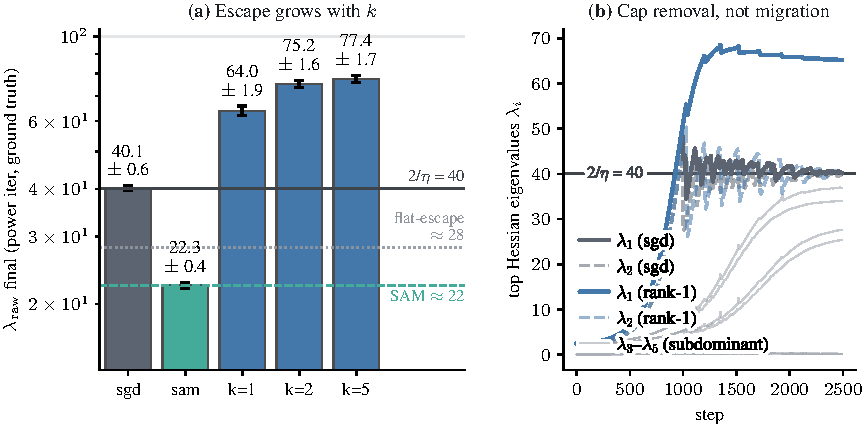
\includegraphics[width=0.95\linewidth]{29_multisharp_migration.pdf}
\caption{Multi-sharp landscape test ($n=5$ seeds). A constructed multi-output
isotropic teacher--student pins \emph{two} directions at $2/\eta$
($\lambda_{1}\!=\!40.1$, $\lambda_{2}\!=\!40.0$). Left: final \lraw\ across
seeds (mean$\pm 95\%$ CI); damping only $u_{1}$ (rank-1) lets $u_{1}$ escape
upward while $\lambda_{2}$ stays pinned: no flow in this constructed test,
inconsistent with migration where it could plausibly act. Right: seed-0
top-eigenvalue trajectories; $k>1$ now matters, revealing the per-direction
structure of the self-stabilization cap. Full values and protocol are given
in \S\ref{app:multisharp}.}
\label{fig:multisharp}
\end{figure}

\FloatBarrier

\section{Stochastic-regime measurement and robustness details}
\label{app:stoch}

\subsection{Cross-batch sensing and descriptive boundary organization}\label{sub:crossbatch}
\textbf{What the fixed-batch reference measures. A cross-batch
sensing study.} All reference measurements above (and the control law's
sensing) use one fixed 512-example batch, so two questions arise: is that
batch's \lref\ representative, and is its top eigenvector the sharp
direction of the \emph{current} minibatches the optimizer actually sees?
We re-ran vanilla SGD with an instrumented protocol ($n{=}3$, same
deterministic driver) that measures, at every outcome step, the ARPACK
top-3 on two additional fixed 512-example batches (seeds 124/125) and on
the \emph{current training minibatch} (bs 128). Late-window results:
(i) the fixed batches \emph{agree at the eigenvalue level} (late \lref\
$28.61\pm3.42$ / $28.12\pm0.83$ / $32.20\pm2.40$ across the three
batches), so the reference protocol is sound as a scalar measurement;
(ii) the current-minibatch $\lmax(H_{B})$ sits markedly higher, $37.0\pm9.7$
(per-measurement median $37$, IQR $[30,48]$), straddling the heavy-ball
reference line at $38$ (Fig.~\ref{fig:bsharp}); and (iii) the top eigenspace is
substantially batch-specific late in training: the reference batch's
$v_{1}$ overlaps the current minibatch's $v_{1}$ with
$|\cos|$ median only $0.26$ (IQR $[0.13,0.51]$; vs.\ $0.47$--$0.53$
against the other fixed batches; top-3 subspace min-cosines
$0.10$--$0.31$). Early and mid training the overlap is high
($|\cos|\!=\!0.89$/$0.90$ median): the shared sharp direction
fragmentates as the spectrum flattens. Consequence: a fixed-batch-sensed
$\hat v_{1}$ is \emph{not} the current minibatch's sharpest direction
late in training, so the rank-1 edit acts on a direction with small
gradient share per step, which is one candidate mechanism for the
single-direction null below. The current-minibatch-sensing control
tests it by intervention (below).

\textbf{Thresholds: which boundary each diagnostic straddles.} The two
reference lines, the momentum-free $2/\eta$ and the heavy-ball
reference line $2(1{+}\mu)/\eta{=}38$, sit at different relations to the three
diagnostics: the batch sharpness ($20.51$) is centered near $2/\eta$, the
fixed-batch \lref\ ($28.6$) sits below $38$, and the current-minibatch
$\lmax(H_{B})$ ($37.0$) straddles the heavy-ball reference line. One reading must be ruled
out explicitly: taking the
minibatch $\lmax(H_{B})$ ``straddling $38$'' as an independent confirmation of
stochastic EoS conflates $\lmax(H_{B})$
with the batch sharpness; the directional quantity the EoSS theory
constrains sits near $2/\eta$ in this protocol, not at the heavy-ball
reference line: an empirical point in the batch-size-dependent regime family of
momentum EoSS \citep{andreyev2026momentum}, in which the batch sharpness
plateaus at the noise-dominated small-batch value $2(1{-}\mu)/\eta$ ($=2$
here) and rises to the large-batch heavy-ball plateau $2(1{+}\mu)/\eta$
($=38$) as batch size grows. We do not read $2/\eta$ as a universal
momentum-EoSS threshold: at our particular operating point (bs $128$,
$\mu{=}0.9$) the measured batch sharpness lies near the momentum-free
boundary $2/\eta$, between the two plateaus; mapping that interpolation is
outside our scope (\S\ref{sec:discuss}). The ordering
$\lstep\!<\!\lref(\text{fixed})
\!<\!\lmax(H_{B})$ is also consistent with the weak-actuation diagnostic
from \S\ref{sub:inertness}: the stochastic gradient follows directions
with bulk-scale curvature, while edits confined to the spectral edge
intersect only a small fraction of the per-step gradient.

\begin{figure}[!ht]
\centering
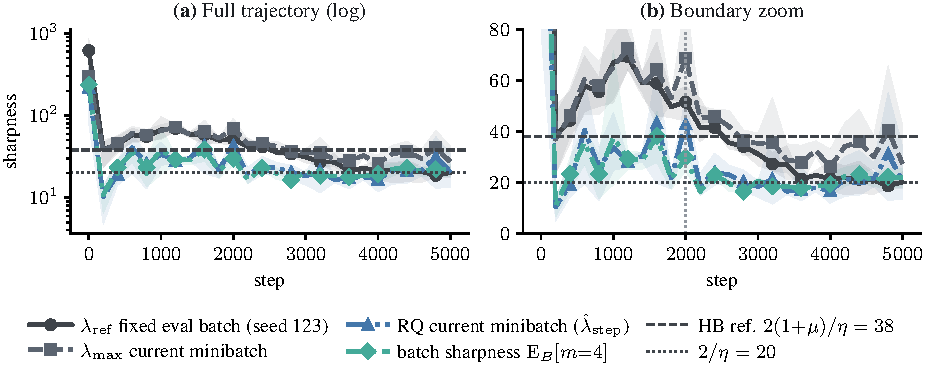
\includegraphics[width=0.95\linewidth]{40_batch_sharpness.pdf}
\caption{Batch sharpness vs.\ spectral sharpness for SGD on
ResNet-18/CIFAR-100 ($n{=}3$ seeds, deterministic protocol; bold curves are
seed means and bands are min--max across seeds). \textbf{(a)} full
trajectories (log scale); \textbf{(b)} boundary-region zoom with the
momentum-free reference $2/\eta$ (dotted) and the heavy-ball reference line
$2(1{+}\mu)/\eta{=}38$ (dashed). The
EoSS batch sharpness $\mathbb{E}_{B}[\mathbf{g}_{B}^{\!\top}H_{B}
\mathbf{g}_{B}/\|\mathbf{g}_{B}\|^{2}]$ ($m{=}4$ minibatches per
measurement) is centered near $2/\eta{=}20$ ($20.51\pm2.10$ late), while
the current-minibatch $\lmax(H_{B})$ ($37.0\pm9.7$) and the
fixed-batch reference \lref\ ($28.6\pm3.4$) are distinct, larger
quantities; late scalar summaries are mean$\pm 95\%$ CI across the three
seeds.}
\label{fig:bsharp}
\end{figure}

\FloatBarrier

\subsection{Batch-sharpness estimator: \texorpdfstring{$m$}{m}-convergence}
\label{sub:mconv}
The $m{=}4$-minibatch average used for
\lstep\ throughout trades Monte-Carlo variance for
cost. At matched end-of-training checkpoints of an independent
re-execution of the canonical SGD protocol (not a bit-replay: nondeterministic
kernels; statistically the same family), the estimator reads
$23.11\pm1.93$ at $m{=}4$ vs.\ $24.40\pm0.43$ at $m{=}16$ and
$24.55\pm0.92$ at $m{=}64$ (mean$\pm$sd, $n{=}3$ seeds):
${\approx}1.4$--$1.5$ units below the $m{=}64$ reference and
${\sim}4.5\times$ the seed spread of $m{=}16$. Every headline
batch-sharpness contrast (e.g.\ SAM$-$SGD $-4.30$, 95\% CI
$[{-}6.70,{-}1.89]$)
exceeds this difference; unresolved contrasts are reported as such.

\paragraph{Subsampling calibration of the $m{=}4$ estimator.}
\label{par:mcal}
We replicate the in-run estimator exactly (same minibatch sampling,
eval-mode BN-frozen convention), draw an $m{=}128$ pool of per-batch
values at each of the three end-of-training SGD checkpoints of the
instrumented rerun, and bootstrap $B{=}2000$ subsamples of size
$m{=}4$ with replacement, matching the i.i.d.\ sampling of the in-run
estimator; a disjoint-partition companion (32 groups of $4$, no reuse)
gives the same conclusion. Table~\ref{tab:mcal} reports the results:
the subsample distributions are centered on the pool estimate
(group-$z$ mean $0.00$, sd $0.93$--$0.94$, $94$--$97\%$ of $|z|<2$),
with dispersion matching the i.i.d.\ prediction $\hat\sigma/2$. The
earlier $m{=}4$ vs.\ $m{=}64$ scan gap ($23.11$ vs.\ $24.55$) is
$0.37\times$ the standard error of an $m{=}4$ estimate: finite $m$
therefore inflates variance without evidence of systematic downward
bias.

\begin{table}[!ht]
\centering\small
\caption{Subsampling calibration of the $m{=}4$ batch-sharpness
estimator at the three end-of-training SGD checkpoints ($m{=}128$
pool per checkpoint; $B{=}2000$ bootstrap subsamples of size $m{=}4$,
with replacement; theory sd is the i.i.d.\ prediction
$\hat\sigma/\sqrt{m}=\hat\sigma/2$ with $\hat\sigma$ the pool sd).}
\label{tab:mcal}
{\renewcommand{\arraystretch}{1.10}\RTableTopGap
\begin{tabular}{lccc}
\toprule
checkpoint (seed) & $\hat\lambda_{128}$ & boot mean$\pm$sd & theory sd \\
\midrule
instrumented SGD rerun, seed 0 & $26.13$ & $26.14\pm4.37$ & $4.36$ \\
instrumented SGD rerun, seed 1 & $24.90$ & $24.99\pm4.52$ & $4.41$ \\
instrumented SGD rerun, seed 2 & $23.01$ & $23.11\pm2.83$ & $2.90$ \\
\bottomrule
\end{tabular}}
\end{table}

\subsection{Spectral redistribution}
\textbf{No persistent spectral redistribution detected at the sampled
checkpoints.} Within the measured top-10 spectrum and the available
checkpoint cadence, we detect no persistent redistribution
sufficient to explain the rank-1 outcome (Fig.~\ref{fig:redist};
$n{=}3$): the
damped direction remains the outcome top eigenvector in $98\%$ of late
measurements (median
$|\cos(\hat v_{\mathrm{ctrl}},v_{1})|{=}0.978$; within the top-5: $100\%$),
the spectrum shows no resolved change: late $\lambda_{2}/\lambda_{1}$ is $0.845$ under
rank-1 damping vs.\ $0.853$ under SGD, with $\lambda_{2}\!\approx\!25.3$ vs.\
$24.4$, and the top-10 subspace turnover between consecutive measurements is
identical (median min-cosine $0.069$ vs.\ $0.070$). Nothing flows: damping
$\hat v_{1}$ neither demotes the damped direction nor lifts $\lambda_{2}$
into a vacancy. The stochastic-regime null is therefore not sharpness
``escaping around'' the edit: at this operating point the edit has
weak per-step actuation ($\sim\!10^{-4}$ gradient share), but
\S\ref{sub:inertness} and the regime sweep show that this diagnostic
alone does not determine the long-horizon response. (This is the stochastic-regime, measured counterpart
of the MLP multi-sharp migration refutation, \S\ref{sub:migration}.)

\begin{figure}[!ht]
\centering
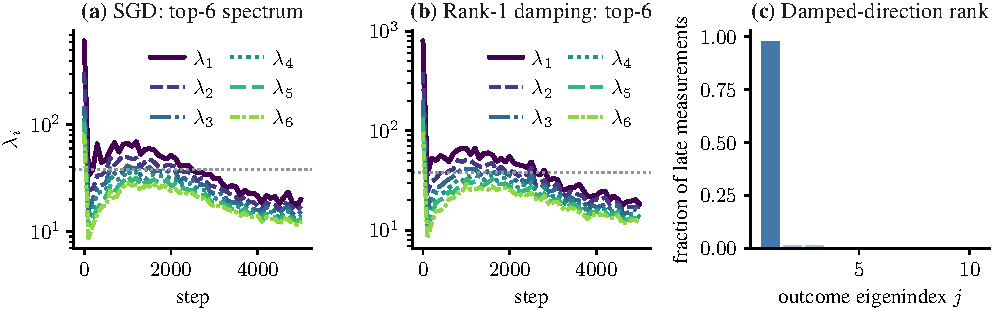
\includegraphics[width=0.95\linewidth]{36_spectral_redistribution.pdf}
\caption{Spectral redistribution test ($n{=}3$ seeds, top-6 outcome spectrum,
seed means). \textbf{(a)} SGD vs.\ \textbf{(b)} accurate rank-1 damping, both
on log-scale y-axes: the
spectra show no resolved difference (late $\lambda_{2}/\lambda_{1}$: $0.845$ vs.\
$0.853$). No sharpness flows into the complement. Eigenvalue index is
encoded redundantly by color and line style. \textbf{(c)} The damped
direction $\hat v_{1}$ remains the outcome top eigenvector in $98\%$ of late
measurements (median $|\cos|{=}0.978$): the edit neither demotes the damped
direction nor lifts $\lambda_{2}$; the top of the spectrum is simply
unperturbed, consistent with the $\sim\!10^{-4}$ per-step gradient share of
the edit.}
\label{fig:redist}
\end{figure}

\subsection{Subspace share at \texorpdfstring{$k{=}50/100$}{k=50/100}}
\label{sub:k100}
Extending the measurement toward the class count evaluates, at matched
canonical checkpoints (eval mode), the cumulative minibatch-gradient
energy share $\mathbb{E}_{B}[\sum_{i\le
k}(\mathbf{g}_{B}\!\cdot\!\hat v_{i})^{2}/\|\mathbf{g}_{B}\|^{2}]$
over $m{=}64$ fresh minibatches against the checkpoint top-$k$
eigenspace ($k$ up to $100$, single ARPACK solve per checkpoint,
${\sim}9$ min per checkpoint). This convention differs definitionally
from the in-run measurement of
\S\ref{sub:inertness}: the checkpoint share is an expectation over
the minibatch distribution against a fixed eigenspace of the
checkpoint Hessian, whereas the in-run $s_k$ is the current single
training gradient's alignment with the live-sensed subspace at that
step (train mode, $k\le20$). Both are correct under their own
conventions: the gap ($s_{20}{=}0.133$ vs.\ ${\lesssim}0.3\%$) is
definitional, not a discrepancy. The checkpoint-share measurement is
also the operationally closer analogue of the persistent dominant
subspace aggregated over training that \citet{song2025bulk} target
(\S\ref{sec:related}); a small in-run share is not inconsistent with
either. Aggregate over $n{=}3$ seeds (mean$\pm$sd):
$s_{20}=0.133\pm0.011$, $s_{50}=0.189\pm0.009$,
$s_{100}=0.239\pm0.010$: no majority of gradient energy resides in
the top eigenspace even at the class count, leaving ${\approx}76\%$
outside the top-$100$ directions.

\subsection{Batch-size $\times$ momentum regime sweep}
\textbf{Exploratory batch-size $\times$ momentum map: asymmetric
re-emergence of the damping effect (Fig.~\ref{fig:regimesweep}).} The deterministic and stochastic regimes so
far sit at two distant operating points. An exploratory sweep
($B\in\{32,128,512,2048\}\times\mu\in\{0,0.9\}$, $n{=}3$, canonical
5000-step protocol, lr not rescaled with $B$; sensing runs at every cell,
the edit arms run at the critical cells $\{128/\mu{=}0,\,512/\mu{=}0.9,\,
2048\times\}$; the $(128,0.9)$ anchor is the cell above) samples
intermediate operating points between them with
four measurements per cell: the gradient-energy share of the edited top-1
subspace, the paired outcome of each edit sign, the EoSS batch
sharpness, and the reference \lref\ (pre-registered predictions and
window rules in the supplement; because fixed steps confound epochs
($3.2\!\to\!205$ epochs across $B$) and momentum shifts convergence speed
by $(1-\mu)^{-1}$, $B\!\le\!128$ cells use the late window and $B\!\ge\!512$
cells the training-phase mid window). We consequently treat this
experiment as an \emph{exploratory phase map}, not as an estimate of a
universal regime boundary. The main observation is \emph{asymmetric}
(Fig.~\ref{fig:regimesweep}b): rank-1 \emph{damping} shows a
statistically resolved shift toward higher sharpness where the dynamics
turn quasi-deterministic---paired $\Delta{=}{+}44.0$, 95\% CI
$[{+}39.6,{+}48.4]$ at $B{=}2048/\mu{=}0.9$, in the direction the 2-D
reduction predicts for damping (the boundary moves \emph{up})---while
at $B{=}128/\mu{=}0$ the point estimate is also positive (${+}49.7$,
95\% CI $[{-}4.2,{+}103.5]$) but is not statistically resolved at the
95\% level, and rank-1 \emph{amplification}
shows no statistically resolved effect toward lower sharpness at \emph{any} tested $(B,\mu)$. Strikingly, the
gradient-energy share barely moves across the sweep
($2.1{\times}10^{-4}$ at $B{=}128$ vs.\ $4.6{\times}10^{-4}$ at $2048$,
$\mu{=}0.9$): what returns at the quasi-deterministic end is not per-step
gradient share but outcome sensitivity, and it returns only in the
reduction's predicted harmful direction. Across the tested batch-size
sweep, only SAM exhibits the lower-sharpness response;
\S\ref{par:rhosweep} provides a pathwise decomposition of the ResNet
linSAM--SAM endpoint gap. Two boundary facts complete the phase picture
(Fig.~\ref{fig:regimesweep}c--d): the near-$2/\eta$ anchor is a special interior
point---at $\mu{=}0.9$ the batch sharpness leaves $2/\eta$ in both
directions ($3.9{\pm}1.0$ at $B{=}32$; $94.8{\pm}42.6$ mid-window at
$512$, above \emph{both} EoSS plateaus, before memorization collapses it
to ${\sim}1$)---and at the tested $\mu{=}0$ operating points the measured batch
sharpness does not concentrate near the deterministic $2/\eta$
reference: it runs $69$–$508$ across $B$ (three- to twenty-five-fold
above it) with healthy optimization throughout (final accuracies
$32$–$50\%$, consistent with each cell's epoch count). We therefore do
not use the deterministic boundary as a descriptive law for these
cells. These cells also caution against treating the deterministic
$2/\eta$ line as a universal descriptive law for the measured
stochastic diagnostic; the reference lines are contextual markers,
not fitted constraints for every cell of the sweep.

\begin{figure}[!htbp]
\centering
\IfFileExists{../figures/45_regime_sweep.pdf}{%
  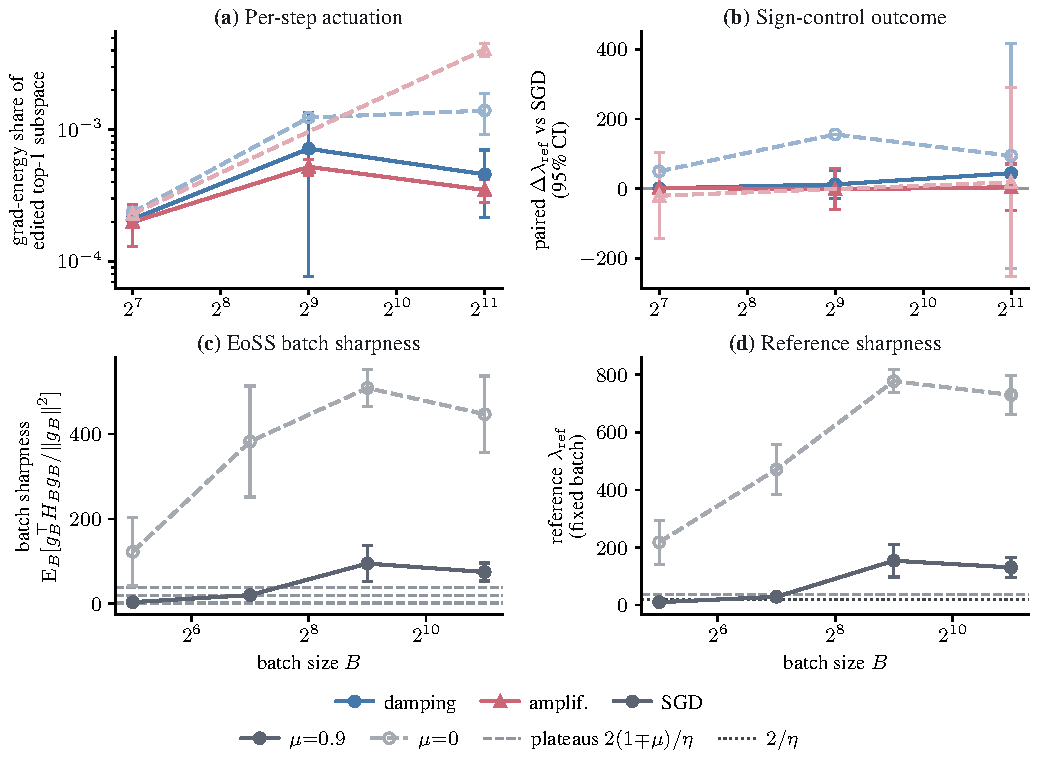
\includegraphics[width=\linewidth]{45_regime_sweep.pdf}}{}
\caption{Regime-transition sweep ($B\in\{32,\!128,\!\allowbreak512,\!2048\}
\times\mu\in\{0,\!0.9\}$, $n{=}3$, canonical protocol; the
$B{=}128/\mu{=}0.9$ anchor reuses the main runs). \textbf{(a)} gradient-energy
share of the edited top-1 subspace (damping/amplifying arms): near-flat at
$10^{-4}$--$10^{-3}$ across the whole range: no monotone return of
per-step effect. \textbf{(b)} paired $\Delta$ reference \lref\ vs.\ SGD with 95\% CIs:
damping (circles) shows a statistically resolved shift toward higher
sharpness at the quasi-deterministic $2048/\mu{=}0.9$ point (${+}44.0$,
95\% CI $[{+}39.6,{+}48.4]$); the $128/\mu{=}0$ point estimate is
positive but not statistically resolved at the 95\% level;
amplification (triangles) is never statistically resolved toward lower
sharpness.
\textbf{(c)} EoSS batch sharpness vs.\ $B$ with the momentum plateaus
$2(1{\mp}\mu)/\eta$: the near-$2/\eta$ anchor is a special point, and the
measured batch sharpness lies several-fold above the deterministic
$2/\eta$ reference at $\mu{=}0$. \textbf{(d)} reference \lref\
(fixed 512-batch ARPACK): decouples from $2/\eta$ at both extremes. Window
rule per supplement: $B{\le}128$ late, $B{\ge}512$ mid (training phase). In
(a), (c), and (d), markers show across-seed means of per-seed window means
and error bars 95\% CIs ($n{=}3$).}
\label{fig:regimesweep}
\end{figure}

\begin{table}[!ht]
\centering
\small
\begin{tabular}{@{}lll@{}}
\toprule
operating point ($B$, $\mu{=}0.9$) & share $s_{1}$ & paired $\Delta\lref$ vs.\ SGD, 95\% CI \\
\midrule
$128$ (canonical, late window) & $2.1\!\times\!10^{-4}$ & $+0.6\;[-3.9,+5.0]$ \\
$512$ (mid window) & $7.2\!\times\!10^{-4}$ & $+12.1\;[-28.6,+52.8]$ \\
$2048$ (quasi-deterministic, mid window) & $4.6\!\times\!10^{-4}$ & $+44.0\;[+39.6,+48.4]$ \\
\bottomrule
\end{tabular}
\caption{Exploratory batch-size sweep: one rank-1 damping edit at $\mu{=}0.9$ ($n{=}3$ per cell; Fig.~\ref{fig:regimesweep}).
The gradient-energy share stays near
$10^{-4}$ while the paired outcome shifts from null to sharply positive
as the dynamics turn quasi-deterministic. This sweep is exploratory:
the fixed step budget conflates batch size with epochs seen, and late
windows are used for $B\le128$ but mid windows for $B\ge512$, so it
establishes an outcome-sensitivity contrast rather than a controlled
regime bridge.}
\label{tab:regimebridge}
\end{table}

\FloatBarrier

\subsection{BN-protocol controls: full results}\label{sub:bnproto}
\textbf{BN-protocol controls: BatchNorm bookkeeping alone does not reproduce
the SAM--linSAM separation.} SAM updates the BN running statistics twice per
step (forwards at $\theta$ and $\theta{+}\epsilon$), while the reference
\lref\ is measured in eval mode through those statistics, so BN-state
evolution is a potential contributor to the measured response. Three
bit-verified protocol controls ($n{=}5$, identical protocol) test this
explanation directly. Reproducing SAM's second forward on a pure-SGD update
(\texttt{sgd\_bn2x}) leaves late \lref\ without a statistically resolved
difference from SGD ($26.3{\pm}0.8$ vs.\ $28.6{\pm}3.4$; paired
$\Delta{=}{-}2.1$, 95\% CI $[{-}5.4,{+}1.2]$): the extra BN update alone
does not produce a statistically resolved shift at this power. Supplying
linSAM with SAM's exact BN evolution (\texttt{linsam\_bnmatched}, buffer
trajectories bit-identical to SAM's) produces a modest resolved downward
shift relative to linSAM ($31.7{\pm}1.7$ vs.\ $34.5{\pm}2.1$; paired
$\Delta{=}{-}2.8$, 95\% CI $[{-}5.3,{-}0.3]$) but remains far above SAM
($22.9{\pm}1.6$). Thus matching BN evolution is insufficient to reproduce
the SAM-level reduction, although these controls do not exclude a smaller
BN-state contribution. Because its buffer trajectory is supplied from
the matched SAM run, \texttt{linsam\_bnmatched} is a causal
diagnostic for the BN-state channel rather than a standalone
deployable optimizer. Conversely, freezing the running statistics in the
official \texttt{disable\_running\_stats} style (\texttt{sam\_bnfreeze})
keeps the training dynamics but raises the measured \lref\ to
$74.2{\pm}4.1$, confirming that the running-stat channel can materially
affect the measured reference sharpness.

\subsection{ViT control: full results}
\textbf{ViT control: the re-query requirement is not universal across the
tested systems.} The ResNet controls establish that the transition
along the tested
interpolation family cannot be reproduced without the finite re-query
at the BatchNorm/CIFAR-100 operating point, but they do
not imply that every stochastic system requires this component. We
repeat the central four arms on ViT-tiny (LayerNorm, no running
statistics) at two operating points. At the below-EoS point
($\eta{=}0.01$ so $2/\eta{=}200$; $n{=}3$), SAM ($21.1{\pm}0.5$) and its
linearization ($21.5{\pm}0.5$) show no statistically resolved difference
from each other,
both far below SGD ($40.4{\pm}2.8$), with rank-1 damping in between
($36.3{\pm}0.5$, within the SGD seed envelope at this power). To obtain
a matched high-curvature operating point with $\lref$ near $2/\eta$
requires the batch-size knob rather
than the learning rate: at bs 128, an lr sweep over $[0.02,0.2]$ leaves
the late $\lref/(2/\eta)$ at $0.34$--$0.41$ with
$\eta\,\lref\approx0.7$--$0.8$ across a $10\times$ lr range (an
lr-independent sub-EoS equilibrium), whereas at bs 512 and lr $0.05$
the late median settles at $0.96\times 2/\eta$ across seeds
($0.95/1.08/0.84/0.98/0.94$; still below the heavy-ball
reference line $2(1{+}\mu)/\eta$). At that matched high-curvature operating point
($n{=}5$) the ordering that isolates
this component is reproduced: SAM separates below SGD ($23.3$ vs.\
$38.4$ late medians; paired $\Delta{=}{-}15.1$, 95\% CI
$[{-}19.9,{-}10.3]$). The linearized control retains a small
statistically resolved difference from SAM
($\Delta(\mathrm{linSAM}-\mathrm{SAM}){=}{+}1.7$, 95\% CI
$[{+}1.1,{+}2.3]$) while satisfying the prespecified TOST equivalence
criterion at $n{=}5$ and the $\pm3.8$ margin (90\% TOST CI
$[{+}1.2,{+}2.1]$). Rank-1 damping, which shows no statistically
resolved difference at the below-EoS point, has a positive point
estimate at the matched high-curvature point (paired
$\Delta{=}{+}4.7$, 95\% CI $[{-}1.3,{+}10.6]$): four of five seeds
are positive, with transient peaks up to $2.3\times$ the SGD late
level, the first appearance of the boundary-moving response in the
ViT control, but the effect is not statistically resolved at the
95\% level, and the evidence should not be described as resolved.
Across both operating
points, the linearized control remains close to SAM; at the matched
high-curvature point it satisfies the prespecified equivalence test at
$n{=}5$ and the $\pm3.8$ margin. Thus, the
decomposition of SAM into first-order and nonlinear components is
system-dependent across the two
tested systems; we use
the ViT results to delimit the SAM-account claim, not to extend the
full-batch EoS theory to Transformers. SAM costs ${\sim}2$--$3$ accuracy
points at both budgets ($0.306$ vs.\ $0.336$ below EoS; $0.371$ vs.\
$0.390$ at the matched point).

\subsection{The 200-epoch recipe: full details}
\label{sub:longrecipe}
\textbf{The ordering survives and separates under the full standard
200-epoch recipe.} To provide an external ordering check beyond the
$5000$-step underfitting regime
(\S\ref{sec:discuss}), we re-ran the three-way under the full standard
recipe---$78{,}200$ steps ($200$ epochs), cosine lr $0.1\!\to\!0$, pad/crop +
horizontal-flip augmentation---with exact ARPACK curvature every $5$ epochs
($40$ checkpoints) under the deterministic protocol, $n{=}5$ seeds per arm (a
$100$-epoch $n{=}3$ replication and an intermediate $12000$-step $n{=}2$ run
had already preserved the ordering in point estimate). In the steady window
(epochs 30--120, where cosine lr runs $0.088\!\to\!0.023$ and the annealing
boundary $2(1{+}\mu)/\eta(t)$ is still informative), the ordering is now
separated, not merely preserved in point estimate: SGD $17.91\pm0.92$, rank-1
damping $19.51\pm4.08$, SAM $12.33\pm0.78$; SAM's CI overlaps neither arm,
with paired per-seed $\Delta(\mathrm{SGD})={-}5.58$, 95\% CI
$[{-}6.46,{-}4.71]$. The rank-1 arm remains statistically unresolved
relative to SGD: its paired difference is $+1.60$, 95\% CI
$[{-}2.94,{+}6.14]$, \emph{above} SGD with the point estimate on the
same above-SGD side as every damping arm of the $5000$-step protocol,
and the arm does not satisfy the prespecified equivalence test against
SGD at this sample size and margin, while its
edit fires on $37\%$ of direction-steps, concentrated in the sharpened
phase and disengaging, by the self-gating design, as annealing carries \lref\
below the fixed $2/\eta$ target. This long-recipe arm retains the
fixed target used by the original controller rather than tracking the
time-varying momentum stability reference. It therefore tests the
persistence of the three-way empirical ordering under a standard
training recipe, not an annealed-boundary-tracking controller. As
$\mathrm{lr}\!\to\!0$ the boundary inflates and every arm falls well below it
(Fig.~\ref{fig:long}a), so late-epoch \lref\ ceases to discriminate. Final
accuracies on the full test set show no statistically resolved
difference
($74.7\pm0.5$ / $74.9\pm0.7$ / $75.3\pm0.2$ for SGD / rank-1 / SAM; SAM's
paired accuracy gain $+0.57\pm0.75$pp, CI containing zero, $p{=}0.10$):
under a deployment-grade
recipe the residual sharpness separation yields no statistically resolved
accuracy gain at this
power, consistent with the monitoring-vs-control split being a statement
about sharpness, not about accuracy.

\subsection{Additional figures}
Figures 12--17 collect the supporting visualizations referenced in
\S\ref{sub:longrecipe}, \S\ref{sub:scale} and the full-batch controls, and
\S\ref{sub:rhosweepapp}; they are grouped here to keep the appendix text
sections compact.

\begin{figure}[!ht]
\centering
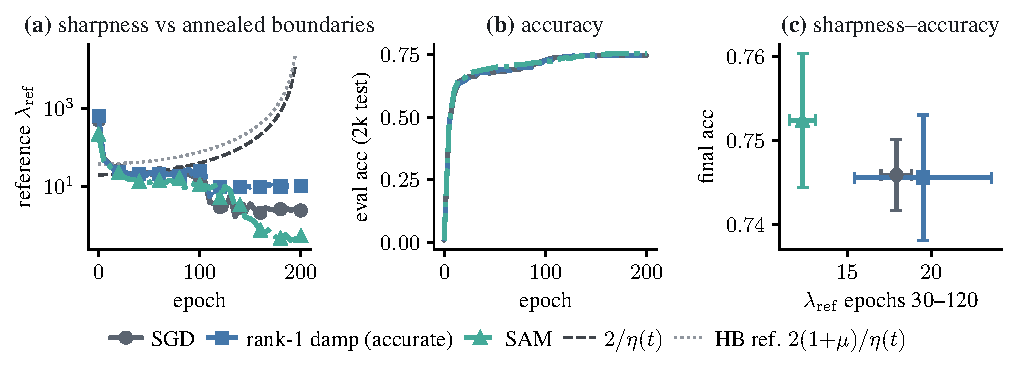
\includegraphics[width=0.95\linewidth]{39_long_recipe_200ep.pdf}
\caption{Standard long recipe, full budget ($200$ epochs, cosine
$0.1\!\to\!0$, pad/crop+flip augmentation, $n{=}5$ seeds, exact ARPACK
curvature every $5$ epochs). \textbf{(a)} Reference \lref\ sits below the
annealed reference curves $2/\eta(t)$ and $2(1{+}\mu)/\eta(t)$ throughout; the arms
can separate, if at all, only in the steady window (epochs 30--120).
\textbf{(b)} Test accuracy (fixed 2{,}000-example test subset). \textbf{(c)} Steady-window \lref\ vs.\ final
accuracy (2k-subset values, mean$\pm$95\% CI): rank-1 damping shows no
statistically resolved difference from SGD
($19.5$ vs.\ $17.9$; paired $\Delta{=}{+}1.6$, 95\% CI
$[{-}2.9,{+}6.1]$); SAM
separates below both ($12.3\pm0.8$; paired
$\Delta{=}{-}5.6$, 95\% CI $[{-}6.5,{-}4.7]$) and shows no statistically
resolved accuracy gain on the full test set (SAM $75.3\pm0.2$ vs.\
$74.7\pm0.5$/$74.9\pm0.7$; paired $+0.57\pm0.75$pp, $p{=}0.10$).
Optimizer identity is encoded redundantly by color, line style, and marker.}
\label{fig:long}
\end{figure}

\begin{figure}[!ht]
\centering
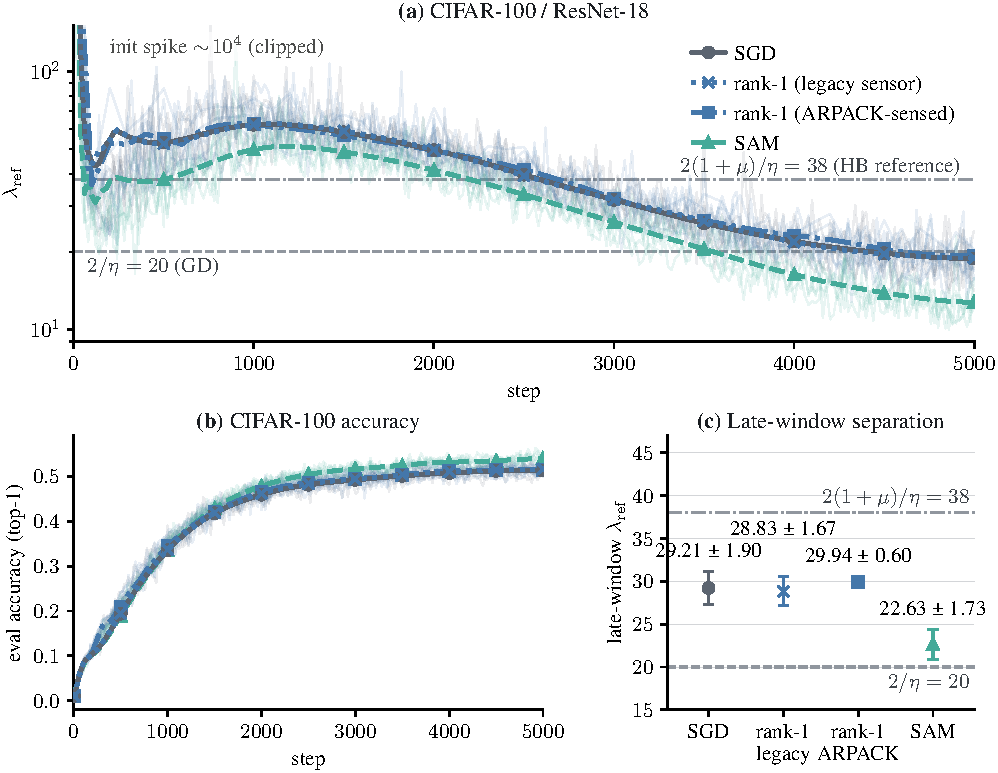
\includegraphics[width=0.95\linewidth]{30_cifar100_r18_control.pdf}
\caption{At-scale reproduction: ResNet-18 (11.2M) on CIFAR-100, deterministic
CUDA, with \lref\ measured by ARPACK on a deterministic 512-sample
evaluation batch. \textbf{(a)} \lref\ trajectories (faint per seed, bold
seed mean; y-axis clipped at $150$ because the initialization transient
reaches ${\sim}10^{4}$) for SGD, the legacy clamped C3 rank-1 arm with the
original sensor, the corrected ARPACK-sensed rank-1 arm (the three
canonical-protocol seeds), and SAM. The GD reference $2/\eta{=}20$ and the
heavy-ball reference line $2(1{+}\mu)/\eta{=}38$ are shown for context.
\textbf{(b)} Evaluation accuracy. \textbf{(c)} Late-window (step
$\geq 2000$) \lref\ mean$\pm 95\%$ CI, per-seed statistics (SGD,
legacy rank-1, and SAM at $n{=}5$ canonical seeds; corrected arm
$n{=}3$): neither rank-1 arm shows a statistically resolved
reduction relative to SGD, while SAM is lower. The
legacy clamped arm fires on $\le\!4\%$ of steps because of the diagnosed
sensing false-convergence; the corrected ARPACK-sensed arm engages
throughout the substantive window (pooled fire rate $93.7\%$ over steps
1--4000, $n{=}3$; five-seed engagement diagnostics in
Appendix~\ref{sub:engagement}) but still shows no statistically resolved
sharpness reduction. \lref\ uses the deterministic+ARPACK protocol; under
the earlier nondeterministic power-iteration measurement the ordering and
CI separation are preserved, while the absolute \lref\ values shift
upward.}
\label{fig:r18}
\end{figure}

\begin{figure}[!ht]
\centering
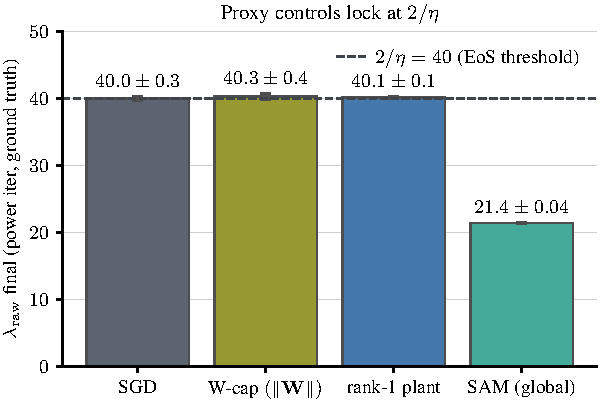
\includegraphics[width=0.62\linewidth]{26_multiseed_control_results.pdf}
\caption{The W-cap and free-lagged rank-1 edit (regime~i) both
lock at $2/\eta$; SAM escapes below it throughout, the sign-flipped
amplifying arm locally (Fig.~\ref{fig:amp}). (The accurate-$v_{\mathrm{top}}$
rank-1 variant, regime~ii, Fig.~\ref{fig:rankk}, instead escapes above
$2/\eta$; the $\gamma$-cap control C2 is reported in the text.) Error bars
are $95\%$ CI ($n{=}5$ for all arms).}
\label{fig:control}
\end{figure}

\begin{figure}[!ht]
\centering
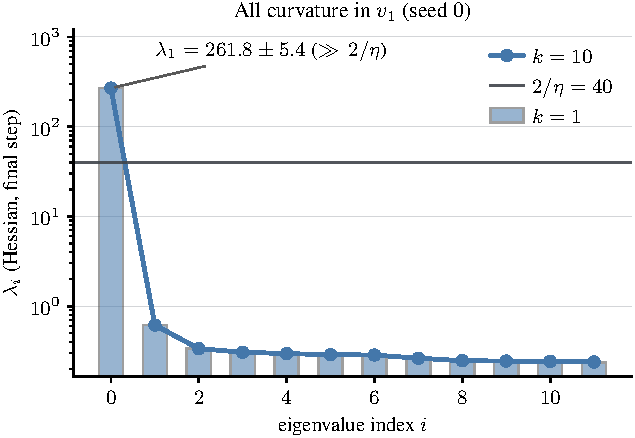
\includegraphics[width=0.62\linewidth]{27_rankk_sweep.pdf}
\caption{Top-$12$ Hessian spectrum of the $1$-D-sharp
teacher--student landscape after unconditional rank-$k$ top-eigenspace
damping with \emph{accurate}
power-iterated $v_{\mathrm{top}}$. The displayed spectrum is seed $0$.
Across $n{=}5$ seeds, the top-eigenvalue summary is
$\lambda_{1}\!=\!261.8\!\pm\!5.4$ (mean$\pm 95\%$ CI), while
$\lambda_{2}\!\approx\!0.6$; thus the spectrum is effectively
one-dimensionally sharp. There is therefore nowhere for sharpness to
migrate to in this testbed, consistent with the $k$-invariance
($k{=}1,2,5,10$ bit-identical; text) predicted by cap removal and
inconsistent with a migration account in which additional damping lowers
\lraw.}
\label{fig:rankk}
\end{figure}

\begin{figure}[!ht]
\centering
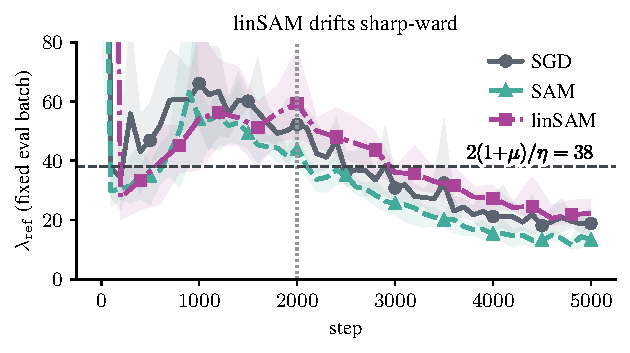
\includegraphics[width=0.62\linewidth]{41_linsam.pdf}
\caption{The full-rank linearized-SAM control
($\mathbf{g}+(\rho/\|\mathbf{g}\|)H_{B}\mathbf{g}$, $\rho{=}0.05$
matched to SAM; $n{=}5$ seeds, bands min--max; SGD/SAM references
$n{=}5$; late window $\geq2000$). The first-order correction, which
amplifies positive-curvature components (and attenuates
negative-curvature ones), does \emph{not} reproduce SAM: linSAM lands at
$34.49\pm2.05$, \emph{above} SGD
($\Delta{=}{+}5.27$, 95\% CI $[{+}1.94,{+}8.61]$) and ${\sim}12$ above SAM, the
same drift toward higher sharpness as rank-$k$ amplification. The
remaining linSAM--SAM transition in this tested BatchNorm ResNet
regime requires the finite re-query residual along the interpolation
of \S\ref{sub:sammech}; increasing the rank of the first-order
correction alone does not reproduce it.}
\label{fig:linsam}
\end{figure}

\begin{figure}[!ht]
\centering
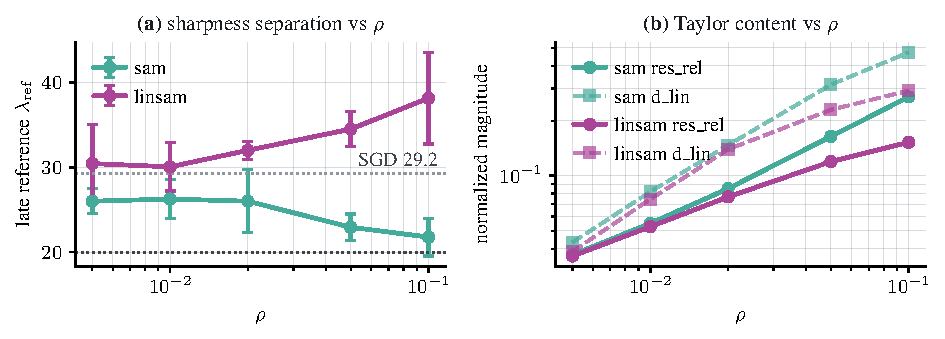
\includegraphics[width=0.95\linewidth]{44_rho_sweep.pdf}
\caption{$\rho$-sweep, full SAM vs.\ linearized SAM
($\rho\in\{0.005,0.01,0.02,0.05,0.1\}$; $n{=}3$ per new $\rho$, $n{=}5$
at linSAM $\rho{=}0.05$; late window $\geq2000$).
\textbf{(a)} late reference \lref\ vs.\ $\rho$ (log axis; SGD
$29.21\pm1.90$ dotted): SAM shows an overall decreasing trend toward
lower sharpness; under the 95\% paired-CI criterion, its first
statistically resolved separation from SGD occurs at the $n{=}5$
canonical cell $\rho{=}0.05$, while the $n{=}3$ sweep cells at
$\rho\in\{0.005,0.01,0.02\}$ remain unresolved at this level. linSAM
shows an overall increasing trend, with the upward separation
statistically resolved from $\rho{=}0.02$: the
separation never inverts and generally widens with the radius. In (a),
markers show across-seed late-window means and vertical bars 95\% CIs;
paired significance claims use the 95\% CIs defined in
\S\ref{sec:setup}. \textbf{(b)} the re-query's Taylor
content on the current minibatch: nonlinear residual
$\|\nabla L_{B}(\theta{+}\rho\hat{\mathbf{g}})-
(\mathbf{g}+\rho H_{B}\hat{\mathbf{g}})\|/\|\mathbf{g}\|$ vs.\ its
first-order part $\rho\|H_{B}\hat{\mathbf{g}}\|/\|\mathbf{g}\|$
(log-log): the residual remains $0.5$--$0.95\times$ the first-order term
at every tested $\rho$: the first-order expansion is never
parametrically close to the re-query it replaces.}
\label{fig:rhosweep}
\end{figure}

\FloatBarrier

\subsection{Statistics details: TOST margins and detrended correlation}\label{sub:tostmargin}
\textbf{Margin sensitivity.} Because the $1/4$ margin is a design choice,
we recomputed every TOST test at $1/8$ and $1/2$ of the SAM effect. At
the $1/8$ margin, no tested arm satisfies the equivalence criterion,
including $k{=}10$. At the $1/2$ margin, the rank-$1$ damping arm, its
current-minibatch-sensing variant, the $k{=}5$/$k{=}10$ damping arms,
the mild amplification control ($\alpha{=}0.5$), the $\alpha{=}1$
single-direction amplification arm, and the true-$\lmax$ sensing arm
satisfy the criterion at their stated sample sizes. Rank-$k$
amplification at $k{=}5/20$ and the wide-rank damping arms $k{=}2/20$
do not satisfy the criterion at any tested margin; the 200-epoch
rank-$1$ damping arm likewise does not satisfy it at any of the three
tested margins. Amplifying controls show predominantly upward point
estimates, with statistically resolved increases under the 95\%
paired-CI criterion for linSAM from $\rho{=}0.02$ in the sweep and
for rank-$k$ amplification at $k{=}20$ ($+4.88$, 95\% CI
$[{+}0.79,{+}8.97]$); none produces the SAM-like downward shift. Thus
the asymmetric qualitative picture is margin-robust, while the only
damping arm satisfying the prespecified $1/4$-margin criterion at its
stated sample size is $k{=}10$.
Detrended Pearson correlation uses a
rolling-mean (window 5) residual to remove the monotone global trend, the
meaningful quantity when both proxy and $\lmax$ drift.

\subsection{The $\rho$-sweep: per-radius results and figures}
\label{sub:rhosweepapp}
Per-radius late reference \lref: full SAM $26.0\,/\,26.3\,/\,26.0\,/\,
22.4\,/\,21.8$ at $\rho{=}0.005\,/\,0.01\,/\,0.02\,/\,0.05\,/\,0.1$;
linearized SAM $30.4\,/\,30.0\,/\,32.0\,/\,34.5\,/\,38.1$ over the same
grid. Per-radius paired contrasts (95\% CIs): full SAM's
$\Delta(\text{SAM}-\text{SGD})$
is $-2.59$ $[-5.80,+0.62]$ / $-2.33$ $[-7.32,+2.65]$ / $-2.59$
$[-9.37,+4.20]$ / $-6.29$ $[-8.73,-3.84]$ / $-6.81$ $[-9.85,-3.78]$;
linearized SAM's paired
$\Delta$ vs.\ SGD is $+1.84$ $[-5.32,+9.00]$ / $+1.46$ $[-2.26,+5.18]$ /
$+3.40$ $[{+}0.22,{+}6.57]$ / $+5.27$ $[{+}1.94,{+}8.61]$ / $+9.54$
$[{+}2.60,{+}16.48]$ over the same grid.

\paragraph{Full-rank negative-sign control (linsamneg).}
The arm $\mathbf{g}\leftarrow\mathbf{g}-(\rho/\|\mathbf{g}\|)H_{B}g$
with $\rho{=}0.05$ matched (one HVP per step, no perturbed-point
re-query, BN protocol as linSAM, $n{=}5$) applies the identical
correction magnitude with the sign flipped. Late reference \lref:
$31.29\pm2.07$; paired contrasts ${+}2.07$, 95\% CI $[{-}1.55,{+}5.70]$
vs.\ SGD (this arm does not satisfy the prespecified equivalence test
at the stated sample size and margin) and ${-}3.20$, 95\% CI
$[{-}5.96,{-}0.44]$ vs.\ linSAM. Batch
sharpness: $20.85\pm0.93$, paired ${+}0.43$, 95\% CI $[{-}2.73,{+}3.59]$
vs.\ the
instrumented SGD rerun ($n{=}3$), at the SGD level. Realized-magnitude
caveat: the arm is step-wise norm-matched by construction, but
realized along-trajectory correction magnitudes differ
($0.56\pm0.16$ vs.\ linSAM's $0.23\pm0.03$, late-window Taylor
column) because the trajectories explore different curvature regions.

\paragraph{Update-norm diagnostic.}
\label{par:taunorm}
Could the monotone interpolation response of \S\ref{sub:sammech} be
an effective-step-size artifact? We reconstruct $\|g_\tau\|$ from the
per-step instrumentation of the interpolation arms; the endpoints are
bitwise identical to the independent \texttt{sam} and
\texttt{linsam\_bnmatched} runs (dedicated $60$-step validation
contracts, metrics and jsonl agreeing to machine precision). Under
the pre-update semantics (the norm that defines the effective step
$\eta\|g_\tau(\theta_t)\|$), the directly instrumented late-window means
are $1.690/1.692/1.646$ at $\tau=0/0.25/0.5$ (cross-seed sd
$0.03$--$0.08$, $n{=}5$), a $2.7\%$ span relative to $\|g_{\rm lin}\|$.
The $\tau{=}1$ arm has no per-step jsonl, so its pre-update norm is not
treated as a direct measurement. A cross-arm validation gives $1.657$
with a matched spread of $6.4\%$ at p50, consistent with the directly
logged range but used only as a validation point. A secondary
semantics that instead closes the reconstruction at the Taylor point
$\theta_{t+1}$ shows a monotone $-10.2\%$ trend, but that semantics
mixes in the post-descent contraction of the same-batch gradient
(measured $G'/G\approx0.58$ late), an outcome of the step's
aggressiveness, not a cause. The available pre-update diagnostic
therefore does not indicate a large effective-step-size change along
the tested interpolation. The
quantitative record behind Fig.~\ref{fig:tau}: at
$\tau=0/0.25/0.5/1$ (mean$\pm$95\% CI, $n{=}5$), late \lref\ is
$31.70\pm1.70\to29.77\pm1.14\to27.45\pm2.56\to22.93\pm1.56$ and
$\lstep$ is
$19.91\pm2.55\to18.94\pm0.92\to17.70\pm1.25\to16.24\pm0.50$; the
paired $\lstep$ contrast $\tau{=}1$ vs.\ $\tau{=}0$ is $-3.67$ with
95\% CI $[-5.95,-1.39]$.

\begin{figure}[!ht]
\centering
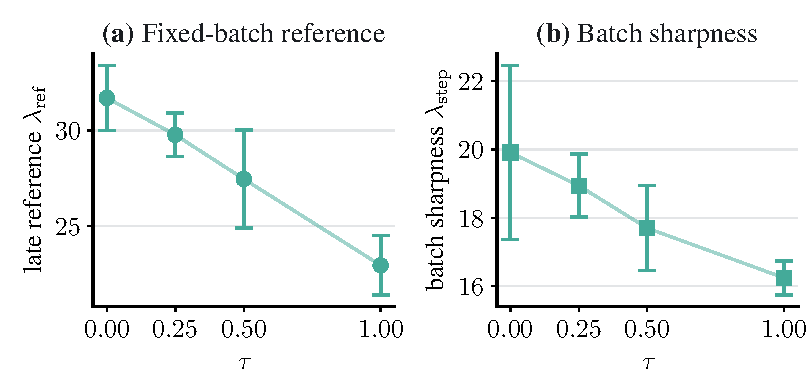
\includegraphics[width=0.62\linewidth]{46_tau_interpolation.pdf}
\caption{Finite re-query interpolation, on both sharpness quantities.
\textbf{(a)} Late fixed-batch reference sharpness $\lref(\tau)$
($t\ge2000$, fixed-512 ARPACK estimate) and \textbf{(b)} EoSS batch
sharpness $\lstep(\tau)$ ($t\ge2000$, $m{=}4$ minibatches),
mean$\pm$95\% CI ($n{=}5$ at every $\tau$), under
$g_\tau=g_{\rm lin}+\tau(g_{\rm SAM}-g_{\rm lin})$ at fixed
$\rho{=}0.05$. The sampled arm means of both responses decrease
across the four tested $\tau$ values; endpoints are
BN-matched linSAM ($\tau{=}0$) and full SAM ($\tau{=}1$). Across the
directly instrumented $\tau\in\{0,0.25,0.5\}$ arms, the late-window
pre-update norm spans $2.7\%$; the $\tau{=}1$ norm is cross-arm
validated rather than directly logged (see the update-norm diagnostic
in this subsection).}
\label{fig:tau}
\end{figure}

\subsection{Rank interpolation: full table and figure}
Table~\ref{tab:interp} gives the full rank-interpolation statistics, and
Figure~\ref{fig:interp} visualizes the same ARPACK-sensed rank-$k$ sweep.
In Table~\ref{tab:interp}/Fig.~\ref{fig:interp}, the legacy label
``damping'' denotes the no-floor raw-divisor signed rescaling for
$k{>}1$; only the corrected rank-1 arm is a pure attenuation test in
practice.

\begin{table}[!ht]
\centering\small
\caption{Rank interpolation at ResNet-18/CIFAR-100 scale (deterministic
protocol of \S\ref{sub:scale}; late reference \lref, step $\geq2000$,
mean$\pm$95\% CI; SGD $29.21\pm1.90$ and SAM $22.63\pm1.73$ at $n{=}5$).
$\Delta$(SGD) is the paired per-seed mean difference with its 95\% CI
for ordinary difference inference. Equivalence is evaluated separately
by TOST at $\alpha{=}.05$, using the corresponding 90\% CI against the
prespecified $\pm1.645$ margin; at this margin and the stated sample
sizes, only the $k{=}10$ damping arm satisfies the equivalence
criterion. fired is the per-direction fraction of edits with
realized damping/amplification factor $>0.1$; share is the edited subspace's
fraction of the instantaneous gradient energy,
$\sum_{i\le k}\cos^{2}(\mathbf{g},\hat v_{i})$; amplification edits are
applied unconditionally every step, so fired is not applicable to them
(n.a.). $n{=}3$ seeds per damping arm; $n{=}5$ for the amplifying arms
$k\in\{5,20\}$.}
\label{tab:interp}
{\renewcommand{\arraystretch}{1.14}\RTableTopGap\RTableDenseRules
\begin{tabular}{llcccc}
\toprule
arm & $k$ & late \lref\ & $\Delta$(SGD), 95\% CI & fired & share \\
\midrule
damping & 1  & $29.94\pm0.60$ & $+1.36\;[-2.28,+5.00]$ & $0.80$ & $2.0\!\times\!10^{-4}$ \\
damping & 2  & $29.13\pm4.15$ & $+0.55\;[-6.41,+7.51]$ & $0.74$ & $4.2\!\times\!10^{-4}$ \\
damping & 5  & $28.82\pm5.62$ & $+0.24\;[-3.34,+3.82]$ & $0.60$ & $9.3\!\times\!10^{-4}$ \\
damping & 10 & $29.47\pm3.41$ & $+0.88\;[-0.20,+1.97]$ & $0.38$ & $1.8\!\times\!10^{-3}$ \\
damping & 20 & $30.23\pm4.34$ & $+1.65\;[-1.98,+5.27]$ & $0.20$ & $2.9\!\times\!10^{-3}$ \\
\midrule
amplify $\alpha{=}1$ & 1  & $28.73\pm0.82$ & $+0.15\;[-3.64,+3.93]$ & n.a. & --- \\
amplify $\alpha{=}1$ & 5  & $31.22\pm2.42$ & $+2.01\;[-0.74,+4.76]$ & n.a. & $8.4\!\times\!10^{-4}$ \\
amplify $\alpha{=}1$ & 20 & $34.09\pm2.28$ & $+4.88\;[+0.79,+8.97]$ & n.a. & $2.6\!\times\!10^{-3}$ \\
\bottomrule
\end{tabular}}
\end{table}

\begin{figure}[!ht]
\centering
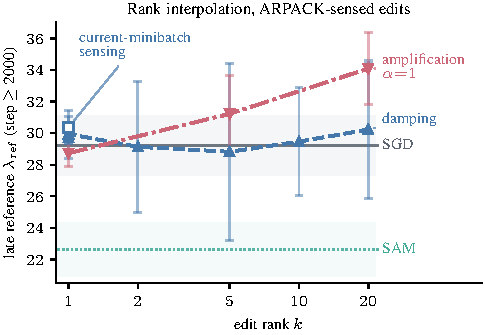
\includegraphics[width=0.62\linewidth]{35_rankkx_interpolation.pdf}
\caption{Rank interpolation (ARPACK-sensed rank-$k$ edits, deterministic
protocol; damping arms $n{=}3$, amplifying arms $k\in\{5,20\}$ $n{=}5$;
late reference \lref\ mean$\pm$95\% CI; SGD/SAM
bands shaded, $n{=}5$). Damping arms (blue) sit inside the SGD band at every
$k\in\{1,2,5,10,20\}$: no descent below the SGD band at any tested rank; the
current-minibatch-sensed control (open markers, \S\ref{sub:scale}) coincides. Rank-$k$
amplification (rose, $\alpha{=}1$) drifts \emph{above} SGD as $k$ grows: the
direction of increasing sharpness, away from SAM. The edited subspace carries
$\le\!0.3\%$ of the per-step gradient energy at every $k$ (Table
\ref{tab:interp}): single-subspace edits produce no statistically resolved $\lref$
reduction at this
operating point at any tested rank. Only $k{=}10$ satisfies the
prespecified equivalence criterion at this sample size and the
$\pm1.645$ margin (paired $\Delta{=}{+}0.88$; 90\% TOST CI
$[{+}0.15,{+}1.62]$); the ordinary paired difference and its 95\% CI
are reported in Table~\ref{tab:interp} (full table:
Appendix~\ref{app:stoch}).}
\label{fig:interp}
\end{figure}

\FloatBarrier

\subsection{Realized actuation strength: full table}
\label{sub:actuationfull}
The per-step realized relative edit
$\|\mathbf{g}'-\mathbf{g}\|/\|\mathbf{g}\|$ is computed exactly from
the per-step plant logs (orthonormal sensed basis): for eigenspace
rescaling edits
$\sqrt{\sum_{i}(f_{i}\cos_{i})^{2}}$ with
$d_{i}=\hat\lambda_{i}/\lambda_{\mathrm{targ}}$ and
$f_{i}=\mathrm{clip}(1-1/d_{i},-1,1)$ on the raw divisor (no
$\max(\cdot,1)$ floor; directions with $d_{i}<1$ thus receive
bounded sign-reversed amplification rather than attenuation) and for
amplification $f_{i}=-\alpha$
unconditionally; angles are exact $\arccos$, no small-edit
approximation. The linSAM/SAM magnitudes are the Taylor columns of the
instrumented reruns (measured every $200$ steps on the current
training minibatch, train-mode BN), so the comparison is
same-order-of-magnitude rather than identically sampled
(\S\ref{sub:scale}, Table~\ref{tab:actuationfull}).

\begin{table}[!ht]
\centering\footnotesize
\setlength{\tabcolsep}{2pt}
\caption{Realized actuation strength, all arms (exact plant statistics
over all $5000$ steps per seed; late window $t\ge2000$; $n$ per arm).
``fired (steps)'' is the fraction of steps on which at least one
direction fires; ``fired (dir.)'' is the per-direction fired fraction
(the ``fired'' column of Table~\ref{tab:interp}); the current-minibatch
rank-$1$ control fires every step. $\|\mathbf{g}'-\mathbf{g}\|/\|\mathbf{g}\|$
is the fired-step mean for the eigenspace edits (amplification is
unconditional) and the late-window mean for the linSAM/SAM corrections
(Taylor-column probes every $200$ steps on the current training
minibatch, train-mode BN), a same-order-of-magnitude, not identically
sampled, comparison. Paired $\Delta\lref$ vs.\ SGD (95\% CIs, from
Table~\ref{tab:interp}) are reported for ordinary difference
inference; equivalence results use separate 90\% TOST CIs as described
in Table~\ref{tab:interp} (current-minibatch control: \S\ref{sub:scale};
linSAM: \S\ref{sub:sammech}; SAM: its $\rho{=}0.05$ radius cell); the
bnmatched arm is not separately contrasted. The strongest eigenspace
edit ($k{=}20$) actuates $3.7\times$ less per step than linSAM and
$5.7\times$ less than SAM, yet only SAM separates downward from SGD.}
\label{tab:actuationfull}
{\renewcommand{\arraystretch}{1.14}\RTableTopGap\RTableDenseRules
\begin{tabular}{llcccccc}
\toprule
arm & $n$ & fired (st.) & fired (dir.) &
$\|\mathbf{g}'-\mathbf{g}\|/\|\mathbf{g}\|$ & angle & late &
paired $\Delta\lref$ \\
\midrule
damp $k{=}1$  & $3$ & $0.80$ & $0.80$ & $0.011$ & $0.6^{\circ}$ & $0.002$ & $+1.36\;[-2.28,+5.00]$ \\
damp $k{=}2$  & $3$ & $0.80$ & $0.74$ & $0.014$ & $0.8^{\circ}$ & $0.003$ & $+0.55\;[-6.41,+7.51]$ \\
damp $k{=}5$  & $3$ & $0.81$ & $0.60$ & $0.018$ & $1.0^{\circ}$ & $0.007$ & $+0.24\;[-3.34,+3.82]$ \\
damp $k{=}10$ & $3$ & $0.83$ & $0.38$ & $0.031$ & $1.7^{\circ}$ & $0.017$ & $+0.88\;[-0.20,+1.97]$ \\
damp $k{=}20$ & $3$ & $0.83$ & $0.20$ & $0.061$ & $3.4^{\circ}$ & $0.035$ & $+1.65\;[-1.98,+5.27]$ \\
\addlinespace[1.5pt]
damp $k{=}1$ (current-minibatch) & $5$ & $1.00$ & $1.00$ & $0.012$ & $0.7^{\circ}$ & $0.008$ & $+1.16\;[-0.69,+3.01]$ \\
\addlinespace[1.5pt]
amp $k{=}5$ ($\alpha{=}1$)   & $5$ & $1.00$ & --- & $0.041$ & $2.3^{\circ}$ & $0.025$ & $+2.01\;[-0.74,+4.76]$ \\
amp $k{=}20$ ($\alpha{=}1$)  & $5$ & $1.00$ & --- & $0.081$ & $4.4^{\circ}$ & $0.045$ & $+4.88\;[+0.79,+8.97]$ \\
\midrule
linSAM ($\rho{=}0.05$)        & $5$ & --- & --- & $0.18$ & --- & $0.23$ & $+5.27\;[+1.94,+8.61]$ \\
linSAM (bnmatched, $\tau{=}0$)& $5$ & --- & --- & $0.18$ & --- & $0.24$ & --- \\
SAM ($\rho{=}0.05$)           & $3$ & --- & --- & $0.28$ & --- & $0.35$ & $-6.29\;[-8.73,-3.84]$ \\
\bottomrule
\end{tabular}}
\end{table}

\subsection{Engagement and eligibility diagnostics: ARPACK-sensed rank-1 damping}
\label{sub:engagement}
Sensing is the first suspect: an optimizer
gating on mini-batch power iteration's $\hat\lambda$ reads
$\approx\!19<2/\eta$ and fires on $\le\!4\%$ of steps ($\approx$ SGD),
but direct ARPACK on a deterministic 512-sample batch gives
$\lref\!\approx\!36$ (median $35.7$, $88\%$ of steps above $2/\eta$):
the $\approx\!19$ was a power-iteration false convergence ($+45\%$ mean
underestimate): the sensing proxy was broken, not the regime. The
legacy clamped arm using this sensor has late
\lref\ $28.83\pm1.67$ ($n{=}5$; Fig.~\ref{fig:r18}).
\emph{With the proxy fixed, the edit fires, and sharpness still shows
no resolved shift.} Warm-started ARPACK sensing ($k{=}2$, every $N{=}20$ steps)
without the $\max(\cdot,1)$ floor gives damping divisor $\approx\!1.8$
and damping factor $\approx\!0.44$ every step; pre-registered
eligibility holds on all $n{=}5$ seeds (divisor median $1.86\geq1.5$;
window-mean damping $+0.39>0.3$; Ritz effective-force rate $100\%$), and
the auxiliary fire-rate criterion over the substantive window too
($98.5\%$, steps 1--4000; $83\%$ over the full 5000, the late dip being
engagement by design). Yet steady \lref\ medians
$[37.2,36.9,39.7,35.6,36.3]$ overlap vanilla SGD ($33.8\pm3.7$).

\subsection{The stochastic-regime amplification arm and current-minibatch sensing: full results}
\textbf{The amplification arm and the current-minibatch-sensing control: no
statistically resolved effect in either direction at this power.} Rank-1 amplification under the identical
deterministic + ARPACK protocol: $\alpha{=}0.5$ ($n{=}5$) and
$\alpha{=}1.0$ ($n{=}3$) both have late \lref\ estimates near the SGD
level ($29.18\!\pm\!1.44$ and $28.73\!\pm\!0.82$ vs.\ SGD
$29.21\!\pm\!1.90$), and neither yields a statistically resolved
downward paired contrast at the stated sample size (accuracies
unmoved, $0.513$--$0.514$ vs.\ SGD's $0.512$), with SAM's
$22.63\!\pm\!1.73$ the
only arm below. The $\alpha{=}1.0$ arm is diagnostic: the momentum-regime
analogue of the 2-D prediction, $2(1{+}\mu)/((1{+}\alpha)\eta)\!\approx\!19$,
sits ${\sim}10$ units below the SGD band, far larger than the
${\sim}1.9$-unit CI, yet no separation occurs (intermittent dips to
${\sim}15$, no sustained shift; $0$ NaN steps). The fixed-batch
confound is excluded by intervention: perhaps the fixed-batch $\hat v_{1}$
(overlap $0.26$) is simply the \emph{wrong} direction, so we re-ran the
accurate damping optimizer with sensing on the \emph{current training
minibatch itself} (ARPACK $k{=}2$ every $N{=}20$ steps; $n{=}5$). The
edit engages even harder (sensed divisor median $2.35$ vs.\
${\sim}1.5$ fixed-batch, realized damping $+0.58$, firing on $100\%$ of
steps) and the outcome shows no resolved change: late reference $\lref =
30.37\pm1.05$, no closer to SAM, accuracies unmoved, the paired point
estimate $+1.16$, 95\% CI $[{-}0.69,{+}3.01]$, \emph{above} SGD with no
reduction in
any seed. Single-direction action thus shows no statistically resolved effect in
\emph{either} sign: under bs-128 noise the training gradient aligns with
\emph{any} top-eigenvector estimate at $|\cos|\!\approx\!0.008$, even
the current minibatch's own, so a rank-1 edit removes only
${\sim}10^{-4}$ of the per-step gradient energy; only full SAM
separates below SGD (whether its first-order expansion alone
reproduces the shift is tested
below; it does not), and the rank-$k$ interpolation remains consistent
with weak per-step actuation through $k{=}20$; as \S\ref{sub:inertness}
shows, however, gradient share alone does not determine the long-horizon
response.

\section{Matched-step X-SAM projector ablation}
\label{app:xsam}

We test whether adding the rank-1 top-eigenvector correction used by X-SAM
\citep{duan2026xsam} on top of SAM produces any further \lref\
reduction. We compare four optimizers on CIFAR-10/ResNet-18 in
\emph{deterministic} CUDA mode ($n{=}10$ seeds; default conv-backward is
non-deterministic: two identical SAM runs diverge to a $\sim\!10^{-1}$
terminal param difference, producing $\sim\!6$-unit spurious \lref\ gaps
that deterministic mode eliminates): SGD, SAM ($\rho{=}0.05$),
\emph{matched-step} X-SAM projector (Duan et al.\ Eq.~11: fixed $\alpha{=}0.2$, no
clamp, sign-gated, unconditional; fires every step), and a \emph{clamped}
variant ($d=\max(\hat\lambda/(2/\eta),1)$, a conservative ablation). We
measure \lref\ by ARPACK on a deterministic 512-sample batch ($k{=}3$,
$\mathrm{tol}{=}10^{-6}$); a mini-batch power-iteration estimate
false-converges on this cross-entropy Hessian, a $+45\%$ mean
underestimate (measured directly), so we report the ARPACK value.

Late-training (step $\geq 3000$) reference \lref, $n{=}10$ mean$\pm 95\%$ CI:
SGD $31.1\pm2.3$, SAM $23.3\pm1.6$, matched-step X-SAM projector
$23.9\pm1.6$, and the clamped projector variant $23.4\pm1.6$ (the three
SAM-family CIs overlap; Fig.~\ref{fig:xsam}a). The paired difference
$\Delta\lref(\text{X-SAM projector}-\text{SAM})$ is $+0.59\pm2.55$
mid-training and $+0.62$ with 95\% CI $[-0.61,+1.85]$ late
(Fig.~\ref{fig:xsam}b). \emph{Thus
no rank-1 effect beyond SAM is resolved at this power; the interval
excludes reductions larger than approximately $0.61$ reference-sharpness
units, while increases up to $1.85$ remain compatible with the data.} We detect none of the substantial \lref\ reduction that Duan
et al.'s ``explicitly constrains \lref'' framing would imply, and no
generalization gain either: final accuracies ($n{=}10$) are SGD $0.802$,
SAM $0.817$, matched-step X-SAM projector $0.814$, clamped $0.815$ (all within
$\pm0.02$ CIs), so the X-SAM projector is not above SAM (it is $0.3$ points below).
Escape is \emph{overwhelmingly} the amplifying SAM component: SAM descends
$\sim\!8$ units below SGD in this CIFAR-10 setting (the CIFAR-100 three-way
of \S\ref{sub:scale} separates by $\sim\!7$) whether or not the rank-1
correction rides on top. (A rank-1-only ablation, no SAM base, was run on
the MLP testbed of \S\ref{sub:rank1}: it escapes past $2/\eta$ to that
section's escape value, $261.8\pm5.4$.)

\textbf{Fidelity to Duan et al.'s protocol.} Our ablation is a controlled
$\lref$-dynamics comparison, not a replication of their accuracy benchmark
(their CIFAR-10/ResNet-18 setting: SGD base, cosine lr $0.1$, weight decay
$5{\times}10^{-5}$, batch $256$, $200$ epochs, flip/pad/crop augmentation,
$\rho{=}0.05$, $\alpha{=}0.2$, $3$ runs; they report X-SAM
$94.71{\pm}0.20$ vs.\ SAM $93.64{\pm}0.30$ there, and $+1.21\%$ average /
$+2.08\%$ maximum across their CIFAR-10 backbones). Three deviations matter.
(i) \emph{Gradient normalization}: their Alg.~2 updates along the
unit-normalized corrected gradient, which decouples step magnitude from the
loss scale; our matched-step arm applies the sign-gated projector
$P_t = I - \alpha\,\mathrm{sign}(\langle g,v\rangle)\,vv^{\top}$ (their
Eq.~11 correction) to the \emph{raw} adversarial gradient so the effective
step size $\eta$ is matched across SGD/SAM/X-SAM projector; with normalized updates
the correction is confounded with a per-step learning-rate change.
(ii) \emph{Schedule}: $5000$ steps (${\sim}13$ epochs) at constant lr $0.1$,
batch $128$, weight decay $5{\times}10^{-4}$, no augmentation, deterministic
CUDA, chosen for seed-level reproducibility ($n{=}10$) rather than peak
accuracy. (iii) \emph{Eigenvector refresh}: warm-started power iteration
($5$ HVPs/step, BN statistics frozen during HVPs) rather than their
intermittent estimation, giving a fresher $v$ and hence if anything a
stronger correction than their protocol. Our null result therefore bounds
the rank-1 correction under matched-$\eta$ dynamics; a full-protocol
replication (cosine schedule, augmentation, normalized updates) remains the
gap between our setting and theirs.

\begin{figure}[!ht]
\centering
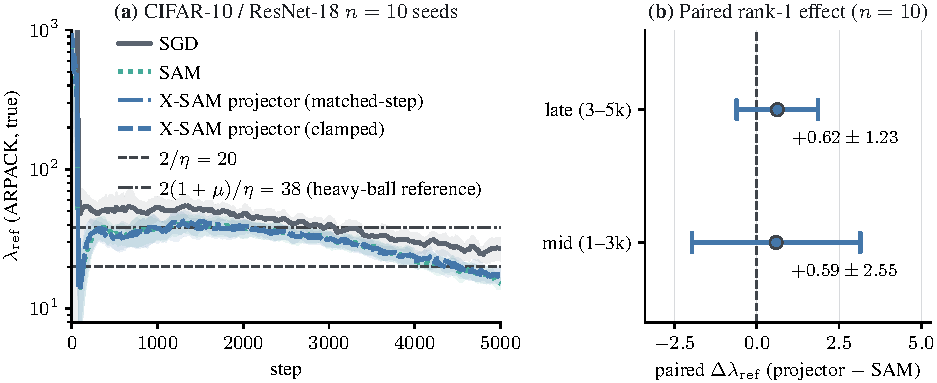
\includegraphics[width=0.95\linewidth]{28_xsam_ablation.pdf}
\caption{Matched-step X-SAM projector ablation on CIFAR-10/ResNet-18
($n{=}10$ deterministic seeds, ARPACK reference \lref).
\textbf{(a)} \lref\ trajectories (bold seed-mean, shaded $95\%$ CI); SAM,
the matched-step X-SAM projector, and the clamped projector variant all
descend below SGD, with the two projector variants close to SAM at this
power. \textbf{(b)} Paired
$\Delta\lref(\text{X-SAM projector}-\text{SAM})$ at mid and late training:
both CIs cross zero (late $+0.62$, 95\% CI $[-0.61,+1.85]$; reductions
beyond ${\sim}0.61$ units excluded), so no rank-1 effect
on \lref\ beyond SAM is detected at this power. The rank-1-only ablation
(no SAM base; MLP testbed, \S\ref{sub:rank1}) escapes upward to
$\lraw\!=\!261.8\pm5.4$.}
\label{fig:xsam}
\end{figure}

\FloatBarrier

\section{Hyperparameters and Compute Cost}
\label{app:hyper}
Tables~\ref{tab:hyper} and~\ref{tab:hyperB} summarize the hyperparameters of the
main experiment families; all values are read from the run manifests and configs.

\begin{table}[!ht]
\centering\footnotesize
\setlength{\tabcolsep}{2pt}
\caption{Hyperparameters of the main experiment families (from run
manifests). All ResNet-18 arms share momentum $\mu{=}0.9$, weight decay
$5{\times}10^{-4}$, batch size $128$, $5000$ steps, lr $0.1$, and (unless
noted) the deterministic-CUDA + ARPACK measurement protocol of
\S\ref{sub:scale}.}
\label{tab:hyper}
{\renewcommand{\arraystretch}{1.05}\RTableTopGap
\begin{tabular}{lp{0.45\linewidth}c}
\toprule
family & configuration & per-run cost \\
\midrule
MLP teacher--student (main) & $n{=}1024$, dim $20$, difficulty (noise std)
$0.3$, teacher $[128,128]$, student $[256,256]$ tanh, full-batch GD, lr
  $0.05$ ($2/\eta{=}40$), $3000$ steps, data seed $1$, $5$ seeds & $\sim$11 s \\
\addlinespace[1.5pt]
Rank-1 amplification control & sign-flip arms $\alpha\in\{0.25,0.5,1\}$
($g'=g+\alpha(g^{\top}\hat v)\hat v$, warm-started block power iteration,
${\sim}3$ HVPs/step, fires every step) $+$ sgd/sam/rankk\_k1 references,
$5$ seeds (\S\ref{sub:amp}) & $\sim$21 s all arms \\
\addlinespace[1.5pt]
Unified fixed-divisor round & fixed-$d$ damping arms
$\eta\in\{0.025,0.05,0.1\}\times d\in\{1.25,1.5,2,2.5,3,6.5\}$
($g'=g-(1-1/d)(g^{\top}\hat v)\hat v$, warm-started block-power-iteration
sensing, fires every step, \emph{no} $\hat\lambda$ feedback), $3000$
steps, single CPU round (float32, torch $2.9.1$; $18$ cells $\times\,5$
model seeds $0$--$4$, data seed $1$) (\S\ref{sub:fixedd},
Fig.~\ref{fig:etad}) & $\sim$50 s per cell \\
\addlinespace[1.5pt]
  Delayed-onset control & adaptive arm to its per-seed gate-opening
  step $T_{\mathrm{gate}}\in\{188,\dots,206\}$ (mean $196.6$), then
  fixed $d\in\{2.5,3\}$; adaptive reference $5/5$ stable
  (\S\ref{sub:fixedd}; Appendix~\ref{app:ampdetails}) & negligible (CPU) \\
\addlinespace[1.5pt]
MLP sweeps & base as main, $4000$ steps; sharpness measured every $50$ steps
(warm-started power iteration, $150$ iters, tol $10^{-4}$; \lraw\ and
$\lambda_{c}$), snapshots every $10$; grids: lr $0.01$--$0.2$ ($20\times$
range), difficulty $0.1$--$1.2$ ($12\times$), width $32$--$256$ ($8\times$) &
$\sim$17 s \\
\addlinespace[1.5pt]
ResNet-18 CIFAR-100 three-way & SGD / rank-1 edit / SAM, $n{=}5$; \lref\ by
ARPACK ($k{=}3$, tol $10^{-6}$) on a deterministic 512-sample eval batch
every $100$ steps & 15--31 min \\
\addlinespace[1.5pt]
X-SAM projector ablation (CIFAR-10) & SGD / SAM ($\rho{=}0.05$) / matched-step X-SAM projector
($\rho{=}0.05$, $\alpha{=}0.2$, sign-gated, no clamp) / clamped variant
($d{=}\max(\hat\lambda/(2/\eta),1)$), $n{=}10$; \lref\ by ARPACK ($k{=}1$,
tol $10^{-6}$, every $20$ steps; every-$100$ $k{=}3$ backups retained) &
29--75 min \\
\addlinespace[1.5pt]
Clamp-free bridge (CIFAR-100) & rank-1 clamp-free (edit factor clipped to
$[-1,1)$, fires every step), $n{=}5$; late-window $\lhatg$ on the
deterministic 512-sample eval batch (\S\ref{sub:bridge}) & 10--45 min \\
\addlinespace[1.5pt]
True-$\lmax$ sensing arm & rank-1 with ARPACK sensing ($k{=}2$, tol
$10^{-2}$, every $N{=}20$ steps on batch $512$), no clamp floor, $n{=}5$
(\S\ref{sub:scale}) & 51--63 min \\
\addlinespace[1.5pt]
At-scale amplification & rank-1 \emph{amplifying} arm with fixed edit
factor $\alpha$ along the sensed direction,
$g{+}\alpha(g^{\top}\hat v)\hat v$; ARPACK sensing as above;
$\alpha{=}0.5$ $n{=}5$, $\alpha{=}1.0$ $n{=}3$ (\S\ref{sub:scale}) &
56--57 min \\
\bottomrule
\end{tabular}}
\end{table}

\begin{table}[!ht]
\centering\footnotesize
\setlength{\tabcolsep}{4pt}
\caption{Additional hyperparameters of the main experiment families
(from run manifests).}
\label{tab:hyperB}
{\renewcommand{\arraystretch}{1.05}\RTableTopGap
\begin{tabular}{lp{0.50\linewidth}c}
\toprule
family & configuration & per-run cost \\
\midrule
Cross-batch sensing study & SGD instrumented with ARPACK top-3 on two extra
fixed 512-batches + the current bs-128 minibatch, $n{=}3$
(\S\ref{sub:scale}) & 26--27 min \\
\addlinespace[1.5pt]
Batch-sharpness measurement & SGD rerun of the cross-batch protocol,
additionally logging the current-minibatch gradient Rayleigh quotient and
an $m{=}4$-minibatch average $\mathbb{E}_{B}[
\mathbf{g}_{B}^{\!\top}H_{B}\mathbf{g}_{B}/\|\mathbf{g}_{B}\|^{2}]$ at
every outcome step, $n{=}3$ (trajectories bit-identical to the cross-batch
study; \S\ref{sub:scale}) & 24 min \\
\addlinespace[1.5pt]
Full-rank linearized SAM & $g\leftarrow g+(\rho/\|g\|)H_{B}g$ with
$\rho{=}0.05$ matched to the SAM arm, $H_{B}$ the current-minibatch
Hessian (one HVP/step, no perturbed-point re-query), $n{=}5$
(instrumented rerun with the batch-sharpness and Taylor-residual logging;
per-step trajectory verified bit-identical
to the uninstrumented runs; \S\ref{sub:scale}) & 30 min \\
\addlinespace[1.5pt]
Negative-sign control & $g\leftarrow g-(\rho/\|g\|)H_{B}g$
with $\rho{=}0.05$ matched (sign-flipped linSAM correction, one
HVP/step, no re-query, BN protocol as linSAM, step-wise
norm-matched), $n{=}5$ (\S\ref{sub:sammech}) & 55--113 min \\
\addlinespace[1.5pt]
Batch sharpness across arms & the central arms rerun with the
cross-batch instrumentation and the $m{=}4$ batch-sharpness estimator:
sam ($n{=}3$), linsam ($n{=}5$), amplify $\alpha{=}0.5$ ($n{=}3$), rank-1
damping ($n{=}3$); sam/linsam additionally log the Taylor residual of the
re-query (\S\ref{sub:scale}, Figs.~\ref{fig:bsarms}, \ref{fig:rhosweep})
& 26--65 min \\
\addlinespace[1.5pt]
$\rho$-sweep, SAM vs.\ linSAM & $\rho\in\{0.005,0.01,0.02,0.1\}$ per arm
($\rho{=}0.05$ from the rows above), $n{=}3$ per new $\rho$, with the
Taylor-residual logging (\S\ref{par:rhosweep}) & 15--20 min \\
\addlinespace[1.5pt]
Current-minibatch-sensing control & rank-1 damping; ARPACK requests the
top 2 eigenpairs on the current minibatch every $N{=}20$ steps for
sensing, while the edit itself is applied only along the leading
eigenvector $\hat v_{1}$; $n{=}5$ (\S\ref{sec:stochastic}) & 34 min \\
\addlinespace[1.5pt]
Rank interpolation & ARPACK-sensed rank-$k$ edits: damping
$k\in\{1,2,5,10,20\}$, amplification $\alpha{=}1$ at $k\in\{5,20\}$
($N{=}20$; $N{=}40$ for $k{=}20$), $n{=}3$ per damping arm and $n{=}5$
for the amplifying arms; $k{=}1$ damping and the SGD
baseline carry top-10 outcome-spectrum instrumentation (the amplify $k{=}1$
row of Table~\ref{tab:interp} is the stochastic-regime amplification arm above)
& 22--99 min \\
\addlinespace[1.5pt]
Long-training validation & three-way (sgd/rank1/sam) rerun, $12000$ steps,
pad/crop + flip augmentation, deterministic + ARPACK, $n{=}2$ seeds; the
standard $100$-epoch recipe ($39{,}100$ steps, cosine $0.1\!\to\!0$,
augmentation, measurement every $5$ epochs, $n{=}3$); and the full standard
$200$-epoch recipe ($78{,}200$ steps, same schedule/augmentation/measurement,
$n{=}5$) (\S\ref{sub:scale}) & 15--297 min \\
\addlinespace[1.5pt]
Regime-transition sweep & $B\in\{2048,512,128,32\}\times\mu\in\{0,0.9\}$
$\times$ \{SGD-sensing reference, rank-1 damping, rank-1 amplification
$\alpha{=}0.5$\}, $n{=}3$; canonical protocol otherwise (lr $0.1$ not
rescaled with $B$; the damping arm's $\lambda_{\mathrm{targ}}{=}2/\eta$ at every
$\mu$); the $(128,\,0.9)$ anchor cell reuses the runs above; batch
sharpness on $m{=}4$ fresh training-batch-size batches
(\S\ref{sub:scale}) & 17--119 min \\
\addlinespace[1.5pt]
ViT high-curvature control & lr grid $\{0.02,0.05,0.1,0.2\}$ @ bs 128 (pilot,
sgd, seed 0) $+$ bs-512/lr-0.05 matched high-curvature point: 4 arms $\times$ 5 seeds
(ARPACK-sensed rank-1 edit $N{=}20$; \texttt{linsam} via a chunked HVP,
128/chunk, LayerNorm-only path), deterministic protocol of
\S\ref{sub:scale} & 14--115 min \\
\bottomrule
\end{tabular}}
\end{table}

\noindent Run-family labels in Tables~\ref{tab:hyper}--\ref{tab:hyperB}
preserve manifest names; interpret $k{>}1$ ``damping'' using the
signed-rescaling semantics of \S\ref{sub:inertness}.

\paragraph{Compute cost.} All GPU experiments ran on a single RTX 5080 (16 GB);
the unified MLP fixed-divisor grid was executed as a separate CPU round.
The MLP families complete in seconds per run ($\sim$11--17 s, from
manifests), while the unified fixed-divisor grid contains $18$ cells
$\times\,5$ model seeds; Table~\ref{tab:hyper} reports its per-cell CPU
cost. The ResNet-18 families dominate the GPU budget: deterministic ARPACK three-way
($15$ runs) ${\sim}5.2$ h; CIFAR-10 X-SAM projector ablation ($40$ runs) ${\sim}33$ h;
ARPACK-sensing edit ($5$ runs) ${\sim}4.6$ h; clamp-free bridge
${\sim}1.9$ h; the cross-batch/rank-interpolation/long-recipe queue ($38$
runs) ${\sim}40$ h; the $200$-epoch external-validity queue ($15$ runs)
${\sim}31.8$ h; batch-sharpness + linearized-SAM controls ($6$ runs)
${\sim}2.2$ h; the batch-sharpness-across-arms + $\rho$-sweep + $n{=}5$
top-up queue ($44$ runs) ${\sim}24.5$ h; and the regime-transition sweep
($46$ runs incl.\ pilot corners and one GPU-timeout re-run) ${\sim}55$
h, roughly $199$ GPU-hours in
total for the ResNet-18 runs reported here (an order-of-magnitude estimate
from run manifests; per-run times vary with GPU sharing).

\FloatBarrier

\section{Detailed scope and limitations}
\label{app:limits}
This appendix collects the full intervention- and
measurement-specific scope statements summarized in
Section~\ref{sec:discuss}. Our claims are deliberately intervention-
and measurement-specific. Lemma~\ref{prop:boundary} is an
orbit-location statement conditional on the 2-D reduced recurrence
(assumptions and gaps G1--G5: Appendix~\ref{app:theory}); the
corresponding period-2 orbit is repelling under the full 2-D
Jacobian, so the theory does not explain attraction, basin size, or
network-level convergence. The fixed-divisor grid therefore tests
only the location prediction on trajectories that exhibit the
corresponding sign-flip behavior; survival is non-monotone and
numerically sensitive near the boundary. The full-batch experiments
use a synthetic tanh teacher--student system with one data
realization and multiple model seeds, so they establish a controlled
mechanistic testbed rather than broad architectural generality.

In the stochastic experiments, $\lref$ is a fixed-batch, eval-mode,
BatchNorm-state-dependent diagnostic, and the $\lstep$ estimator
freezes BatchNorm statistics in eval mode; neither quantity is
asserted to be a parameterization-invariant or exact train-mode
stability variable for every optimizer arm. The $2/\eta$ target of
the stochastic rescaling controller is an intervention convention
inherited from the full-batch construction, not a theoretical
momentum boundary, and the periodically refreshed
current-minibatch-sourced control does not provide per-step
same-minibatch oracle sensing. The rank-1 attenuation null and the
wider raw-divisor rescaling results cover top-Hessian-eigenspace
edits through $k{\le}20$ at one ResNet-18/CIFAR-100 operating point
and one ViT-tiny cross-system control that does not isolate
architecture, normalization, dataset, or protocol; together with the
controlled full-batch MLP, the tested systems leave broader
architectural and dataset generality open. For $k{>}1$ the
raw-divisor rescaling has no $\max(d_i,1)$ floor (above-target
directions are attenuated while below-target directions receive
bounded sign-reversed amplification), and we provide neither a
controlled fixed-strength attenuation sweep nor a norm-matched
random-subspace baseline, so the null cannot be attributed uniquely
to the use of Hessian eigendirections or to the realized strength
and geometry of the tested edits. Several supporting cells use
$n{=}3$ seeds; a statistically unresolved difference is not evidence
of exact equivalence, and equivalence conclusions are sample-size-
and margin-specific. The batch-size sweep changes examples seen and
summary windows and is therefore an exploratory operating-point map,
not a causal estimate of a stochastic-to-deterministic transition.
The canonical ResNet protocol is short, constant-lr, and
augmentation-free; the 200-epoch experiment validates only the
tested SGD/rank-1/SAM ordering under the standard recipe. The tested
intervention families rescale gradient components or compare against
SAM-derived corrections; we do not test direct gradient-based
optimization of $\lmax$ or other higher-order curvature controllers,
so the conclusions concern the tested directional-gradient
interventions, not the controllability of sharpness in general.
Finally, the linSAM--SAM interpolation varies the entire finite
re-query residual bundle and therefore does not isolate which
nonlinear constituent causes the ResNet response; the ViT control
further shows that the decomposition is system-dependent. The paper
is diagnostic rather than algorithm-design work: we use successful
controls such as SAM and full-batch amplification to delimit failure
modes, but do not claim a new optimizer that improves accuracy or
universally reduces sharpness.

\end{document}
